\part{La recta real y el conjunto de los numeros reales \(\R \)}
\section{Numeros reales}
\subsection{Propiedades algebraicas}
En el conjunto \(\R \) de los numeros reales hay dos operaciones binarias, denotadas por \(+ \) y \(\cdot \), a las que se llama adicion y multiplicacion, respectivamente. Estas operaciones satisfacen las siguientes propiedades:
\begin{enumerate}
	\item \((a+ b) + c = a + (b + c )\) para toda \(a,b,c \in \R \) (propiedad asociativa de la suma)
	\item \(a + b = b + a \) para toda \(a,b \in \R \) (propiedad conmutativa de la suma)
	\item existe un elemento \(0 \) en \(\R \) tal que \(0 + a = a \) y \(a + 0 = a \) para toda \(a \) en \(\R \) (existencia del elemento neutro)
	\item para cada \(a \) a en \(\R \) existe un elemento \(-a \) en \(\R \) tal que \(a + (-a) = 0 \) y \((-a) + a = 0 \) (elementos opuestos)
	\item \((a \cdot b) \cdot c = a \cdot (b \cdot c )\) para toda \(a,b,c \) en \(\R \) (propiedad asociativa de la multiplicacion)
	\item \(a \cdot b = b \cdot a\) para toda \(a,b \in \R \) (propiedad conmutativa de la multiplicacion)
	\item existe un elemento \(1 \) en \(\R \) diferente de \(0 \) tal que \(1 \cdot a = a \) y \(a \cdot 1 = a \) para toda \(a \) en \(\R \) (existencia del elemento neutro)
	\item para cada \(a \neq 0 \) en \(\R \) existe un elemento \(a^{-1}\) en \(\R \) tal que \(a \cdot a^{-1} = 1 \) y \(a^{-1} \cdot a = 1 \) (elemento inverso)
	\item \(a \cdot (b + c) = (a \cdot b) + (a \cdot c )\) y \((b + c) \cdot a = (b \cdot a) + (c \cdot a )\) para toda \(a,b,c \in \R \) (propiedad distributiva de la multiplicacion sobre la adicion).
\end{enumerate}
Por satisfacer estas propiedades (axiomas) se dice que el conjunto \(\R \) tiene estructura de cuerpo respecto de la suma y producto habituales, o tambien que la terna \((R,+,\cdot )\) es un cuerpo. Las propiedades anteriores, que constituyen los primeros 9 axiomas de la definicion axiomatica \(\R \), permiten obtener otras propiedades. Algunas de estas son las siguientes:
\begin{itemize}
	\item \(\forall x \in \R \) si \(x + x = x \) necesariamente \(x = 0 \). En efecto, si \(x + x = x \) entonces \((-x) + (x + x ) = (-x) + x \overset{A1}{\Rightarrow} (-x + x) + x = 0 \Rightarrow 0 + x = 0 \Rightarrow x = 0\).
	\item \(\forall a \in \R \) se verifica que \(0a = 0 \). En efecto, \(0a = (0 + 0)a = 0a + 0a \) y, haciendo uso de la propiedad anterior, \(0a = 0 \).
	\item El elemento opuesto de un numero es unico. Supongamos que existen dos elementos \(b,c \in \R \) tal que \(b + a = 0 \) y \(c + a = 0 \). En ese caso, \(a + b = 0 = a + c \) y, por tanto,  \(b = b + 0 = b + (a + c) \overset{A2}{=}(b + a) + c = 0 + c = c \).
	\item \((-1)a = -a \). En efecto, \(a + (-1)a = 1a + (-1)a = (1 + (-1))a = 0a = 0\) por lo que teniendo en cuenta la unicidad del elemento opuesto tenemos que \((-1)a= -a \).
	\item Si \(ab = 0 \) y \(a \neq 0 \), entonces \(b = 0\). Si \(a \neq 0 \) entonces podemos multiplicar ambos lados de la igualdad por \(a^{-1} \), obteniendo \(a^{-1} ab = a^{-1} 0 \Rightarrow 1b = 0 \Rightarrow b = 0 \).
	\item La ecuacion \(ax + b = 0 \) tiene una unica solucion, siempre que \(a \neq 0 \).
\end{itemize}
\subsection{Propiedades del orden}
En el conjunto de los numeros reales se considera una relacion de orden \(\leq \) que tiene las siguientes propiedades:
\begin{enumerate}
	\item[10.] \(\forall a \in \R\), \( a \leq a \) (reflexiva)
	\item[11.] \(\forall a,b \in \R \), si \(a \leq b \) y \(b \leq a \), entonces \(b = a \)
	\item[12.] \(\forall a,b,c \in \R \), si \(a \leq b \) y \(b \leq  c\), entonces \(a \leq  c \).
	\item[13.] \(\forall a,b \in \R \) si \(a,b \in \R \), entonces o \(a \leq b \) o \(b \leq a \) (relación de orden total).
	\item[14.] \(\forall a,b,c \in \R \), si \(a \leq b \) y \(c \in \R \), entonces \(a + c \leq b + c \) (compatibilidad con las operaciones algebraicas).
	\item[15.] \(\forall a,b, c \in \R \), si \(a \leq b \) y \(0 \leq  c \), entonces \(ac \leq bc\).
\end{enumerate}
\begin{remark}
	Hay que tener en cuenta los otros tres simbolos de orden:
	\begin{itemize}
		\item \(a \geq b \) quiere decir \(b \leq a \).
		\item \(a < b \) quiere decir \(a \leq b \) y \(a \neq b \)
		\item \(a > b \) quiere decir \(b < a \).
	\end{itemize}
\end{remark}

A partir de estas propiedades podemos definir los siguientes conjuntos:
\begin{definition}
	\[
		\R^{+} = \set{x \in \R \mid x > 0}
	\]
	\[
		\R^{-} = \set{x \in \R \mid x < 0}
	\]
\end{definition}
\begin{proposition}
	Sean \(a,b \in \R \). Entonces
	\[
		a \leq b \Rightarrow -a \geq -b
	\]
\end{proposition}
\begin{proof}
	\begin{align*}
		a \leq b & \Rightarrow a + (-a) \leq b + (-a) \Rightarrow 0 \leq b + (-a) \Rightarrow -b + 0 \leq -b + (b + (-a)) \\ & \Rightarrow -b \leq (-b + b) + (-a) \Rightarrow -b \leq 0 + (-a) \Rightarrow -b \leq -a \Rightarrow -a \geq -b
	\end{align*}
\end{proof}

\subsection{Intervalos}
Si \(a,b \in \R \) y \(a \leq  b \), entonces se definen:
\begin{itemize}
	\item el intervalo abierto de extremos \(a \) y \(b \) como el conjunto \((a,b) = \set{x \in \R \mid a < x < b }\).
	\item el intervalo cerrado de extremos \(a \) y \(b \) como el conjunto \([a,b] = \set{x \in \R \mid a \leq x \leq b }\)
	\item \([a,b) = \set{x \in \R \mid a \leq  x < b }\)
	\item \((a,b] = \set{x \in \R \mid a < x \leq b}\) (en algunos textos llaman a estos intervalos semiabiertos o semicerrados)
	\item \((-\infty,b) = \set{x \in \R \mid x < b }\)
	\item \((-\infty,b] = \set{x \in \R, x \leq b }\)
	\item \((a,+\infty) = \set{x \in \R \mid a < x}\)
	\item \([a,+\infty) = \set{x \in \R \mid a \leq x }\)
	\item \((-\infty, +\infty) = \R \)
\end{itemize}
% \begin{definition}
% 	Sea \(A \) un subconjunto no vacio. \(m \) es una cota superior de \(A \) si \(a \leq m \; \forall a\in A \).

% 	Diremos que \(A \) esta acotado superiormente si tiene una cota superior. Si \(A \) esta acotado superiormente, diremos que un numero \(M \) es el supremo de \(A \) si:
% 	\begin{itemize}
% 		\item \( a \leq M \forall a \in A \)
% 		\item \(a \leq m \; \forall a \in A \Rightarrow M \leq m\)
% 	\end{itemize}
% \end{definition}
\begin{definition}
	Sea \(S \) un subconjunto no vacío de \(\R \).
	
	\begin{enumerate}
		\item[a)] Se dice que \(S \) está \textbf{acotado superiormente} si existe un numero \(u \in \R \) tal que \(s \leq u \) para todo \(s \in S\). A cada uno de estos numeros \(u \) se le llama cota superior de \(S \).
			
			\item[b)]Se dice que el conjunto \(S \) está \textbf{acotado inferiormente} si existe un numero \(w \in \R \) tal que \(w \leq s \) para todo \(s \in S \). A cada \(w \) se le llama cota inferior de \(S \).
			
		\item[c)] Se dice que un conjunto está acotado si está acotado tanto superior como inferiormente; en caso contrario, se dice que es no acotado.
	\end{enumerate}
\end{definition}

\begin{definition}
	Sea \(S \) un subconjunto no vacío de \(\R \).
	\begin{enumerate}
		\item[a)] Si \(S \) está acotado superiormente, entonces se dice que un numero \(u \) es un supremo de \(S \) si satisface las condiciones:
			\begin{itemize}
				\item \(u \) es una cota superior de \(S \), o equivalentemente, \(s \leq u \;\forall s \in S \).
				\item si \(v \) es cualquier cota inferior de \(S \), entonces \(u \leq v \).
			\end{itemize}
		\item[b)] Si \(S \) está acotado inferiormente, entonces se dice que un numero \(w \) es un infimo de \(S\) si satisface las condiciones: \begin{itemize}
				\item \(w \) es una cota inferior de \(S \), o equivalentemente, \(w \leq s \; \forall s \in S \).
				\item si \(t \) es cualquier cota inferior de \(S \), entonces \(t \leq w \).
			\end{itemize}
	\end{enumerate}
	
	Además, si \(S \) tiene supremo o infimo se les denotará, respectivamente, por
	\[
		\sup S \;\text{ e } \;\inf S .
	\]
\end{definition}
Si \(\sup S \in S\), diremos que es el \textbf{máximo}  de \(S \). Por otro lado, si \(\inf S \in S \), recibe el nombre de \textbf{mínimo}  de \(S \).

Un conjunto \(S \) que no esté acotado superiormente no tendrá supremo (ni cotas superiores). En este caso a veces se escribe que \(\sup A = + \infty \).
% \begin{definition}
% 	Sea \(A \subseteq \R \). Entonces
% 	\begin{itemize}
% 		\item Si \(A \) esta acotado superiormente, decimos que \(\sup(a )\) es el supremo de \(A \) si
% 		      \begin{itemize}
% 			      \item \(a \leq \sup (A) \forall a \in A \)
% 			      \item \(a \leq m \; \forall a \in \R \Rightarrow \sup (A) \leq m \)
% 		      \end{itemize}
% 		\item Si \(\sup (A) \in A \), decimos que es el maximo de \(A \).
% 		\item Si \(A \) es acotado inferiormente, decimos que \(\inf (A) \) es el infimo de \(A \) si
% 		      \begin{itemize}
% 			      \item \(\inf (A) \leq a \; \forall a \in A \)
% 			      \item \(m \leq a \; \forall a \in A \Rightarrow m \leq \inf (A )\)
% 		      \end{itemize}
% 		\item Si \(\inf (A) \in A \) recibe el nombre de minimo de \(A \).
% 	\end{itemize}
% \end{definition}
\subsection{Axioma del supremo}
Para terminar la axiomática de los numeros reales, se añade la siguiente propiedad:
\begin{enumerate}
	\item[16.] Todo subconjunto de los numeros reales no vacio y acotado superiormente tiene supremo.
\end{enumerate}

La propiedad análoga para los infimos se puede deducir a partir del axioma del supremo. Supongamos que \(S \) esta acotado inferiormente. Entonces existe el infimo de \(A \) y se tiene que
\[
	\inf (A) = - \sup (-A )
\]
siendo \(-A = \set{-a \mid a \in A}\).
\begin{proof}
	Veamos que \(\exists \inf (A)\) y \(\inf (A) = - \sup (-A)\). En primer lugar, \(-A \neq \varnothing\) porque \(A \neq 0\). Sea \(m \in \R \) con \(a \geq m \; \forall a \in A\), que existe por estar \(A \) acotado inferiormente. Entonces \(-a \leq -m \; \forall a \in A\), es decir, \(-a \leq -m \; \forall -a \in -A \), con lo que \(-A \) está acotado superiormente y, por el axioma del supremo, existe \(\sup (-A)\). 
	
	Por otro lado, se tiene que \(-a \leq \sup (-A) \; \forall -a \in -A \Rightarrow a \geq -\sup (-A) \; \forall -a \in -A \iff  a \geq - \sup (-A) \; \forall a \in A\), es decir, \(-\sup (-A) \) es cota inferior de \(A \). 
	
	Veamos que \(-\sup (-A)\) es la mayor de las cotas inferiores de \(A \). Sea \(m \in \R\) con \(m \leq a \; \forall a \in A\). Entonces 
	\begin{align*}
		m \leq a \; \forall a \in A & \iff  -m \geq -a \; \forall a \in A \iff -m \geq -a \; \forall -a \in -A \\ & \Rightarrow -m \text{ es una cota superior de } -A \Rightarrow -m \geq \sup (-A) \Rightarrow m \leq -\sup (-A)
	\end{align*}
	Luego, \(-\sup (-A) = \inf (A)\).  
\end{proof}
\section{Números naturales, enteros y racionales}
Los otros tres conjuntos numericos más conocidos son:
\begin{itemize}
	\item Los números naturales \(\N = \set{1,2,3,\ldots }\)
	\item Los números enteros \(\Z = \set{\ldots,-2,-1,0,1,2,\ldots}\)
	\item Los números racionales \(\Q = \set{[\frac{p}{q}] \mid p,q \in \Z, q \neq 0 }\), donde \([\frac{p}{q }]\) es la clase de equivalencia o conjunto de todas las fracciones que representan dicho numero racional. Es decir, \([\frac{p}{q }]\) está formado por \(\frac{p}{q}\) y todas las fracciones \(\frac{s}{t }\) tales que \(\frac{p}{q } = \frac{s}{t }\).
\end{itemize}
Se tiene que \(\N \subset \Z \subset \Q \subset \R \). Los numeros racionales satisfacen los 15 primeros axiomas de \(\R \).

\section{Los numeros irracionales}
El primer problema con las fracciones apareció en la Grecia antigua, en la escuela pitagórica. Estos descubrieron que cantidades muy sencillas como la diagonal de un cuadrado de lado unidad (\(\sqrt{2 } \)) no podian ser expresadas como fracciones.

En particular, la ecuacion \(x^{2 } - 2= 0 \) no tiene solucion en \(\Q \). Ademas, los teoremas basicos del analisis real descansan en la estructura de dichos numeros y la gran mayoria serian falsos si consideramos solo numeros racionales.

Por ejemplo, tiene sentido considerar el resultado de la ``operacion'' \(2^{\sqrt{2} } \)? Sí, pues considerando el conjunto \(A = \set{2^{\frac{p}{q}} \in \R \mid \frac{p}{q } \in \Q \wedge \frac{p}{q } \leq \sqrt{2} }\), que es un conjunto que está acotado superiormente, resultará que \(2^{\sqrt{2 } } = \sup A \). En general, dados \(x,y \in \R \), con \(x > 0 \), se define \(x^{y } \) del siguiente modo:
\begin{itemize}
	\item Si \(x > 1 \) entonces \(x^{y } = \sup \set{x^{r } \mid r \in \Q \mid r \leq y}\)
	\item Si \(x < 1 \) entonces \(x^{y } = \inf \set{x^{r} \mid r \in \Q \mid r \geq y}\)
\end{itemize}
\section{Propiedades topológicas de los numeros reales}
\subsection{Propiedad arquimediana}
\begin{proposition}[Propiedad de Arquimedes]
	El conjunto de los numeros naturales no está acotado superiormente en \(\R \), o equivalentemente, si \(x \in \R \) entonces existe \(n \in \N \) tal que \(x < n \).\footnote{No visto en clase.}
\end{proposition}
\begin{proof}
	Supongamos que \(\N \) esta acotado. Como es un subconjunto de \(\R \) no vacÍo, entonces existirÁ el supremo de \(\N \), al que denotaremos \(p \). Como \(p \) es una cota superior mínima de \(\N \), el numero \(p - 1 \) no puede ser una cota superior, con lo que debe haber algun numero natural \(n \in \N \), de manera que \(p - 1 < n \leq p \). Pero, en ese caso, sumando \(1 \) a \(n \), tendríamos que \(p < n + 1 \), con \(n + 1 \in \N \), por lo que \(p \) no puede ser el supremo de \(\N \).
	
	Hemos llegado a una contradiccion. No hay supremo de \(\N \) y, por tanto, \(\N \) no puede estar acotado.
\end{proof}
A partir de esta propiedad se siguen consecuencias muy importantes que permiten relacionar los naturales, enteros y racionales con los numeros reales:
\begin{proposition}[Propiedad arquimediana de los numeros reales]
	Si \(x,y \in \R \) con \(0 < x \), \(\exists n \in \N \) de manera que \(y < nx \).
\end{proposition}
\begin{proof}
	Consideramos el número real \(\frac{y}{x }\). Como los naturales no están acotados en \(\R \), existirá algun numero natural \(n \) de manera que \(\frac{y}{x} < n \), y multiplicando ambos lados de la desigualdad por \(x \) llegamos a que \(y < nx \).
\end{proof}

\subsection{Principio de los intervalos encajados}
\label{anidados}
Supongamos que tenemos \([a_1,b_1], [a_2,b_2], \ldots, [a_n,b_n],\ldots \) con \(n \in \N \) infinitos intervalos cerrados. Estos intervalos estan encajados cuando se verifica que \([a_n,b_n] \subset [a_{n-1}, b_{n-1}]\), es decir, cuando cada intervalo esta contenido en el anterior. Cuando tenemos infinitos intervalos cerrados encajados ocurre el ``principio de los intervalos encajados de Cantor'': Si \([a_1,b_1], [a_2,b_2],\ldots,[a_n,b_n],\ldots \) son infinitos intervalos encajados, entonces hay al menos un punto comun a todos los intervalos ya que, si consideramos el conjunto \(A = \set{a_n \mid n \in \N }\) formado por todos los extremos izquierdos de los intervalos, al estar todos los intervalos encajados, resulta que:
\[
	a_1 \leq a_2 \leq \cdots \leq a_n \leq a_{n+1} \leq \cdots
\]
De la misma manera resulta que \(a_n \leq b_m \) para cualesquiera \(m,n \in \N \), ya que en caso contrario los intervalos dejarian de estar encajados.

En particular, el conjunto \(A \) es acotado. Sea \(a = \sup A \). Por un lado \(a_n \leq a \), ya que es una cota superior de \(A \). Por otro lado, como cualquier \(b_n \) es cota superior de \(A \), por lo que el supremo sera menor, es decir, \(a \leq b_n \). Esto quiere decir que sea cual sea \(n,a \in [a_n,b_n ]\), y por tanto \(a \) es un punto comun a todos estos intervalos.\footnote{\label{novisto}No visto en clase.}

\subsection{Densidad de \(\Q\) en \(\R \)}
Entre dos numeros reales distintos cualesquirea siempre existe un numero racional (de hecho, infinitos)\textsuperscript{\ref{novisto}}. Concretamente:
\begin{proposition}
	\[
		\forall x,y \in \R, x < y, \exists r \in \Q \text{ tal que } x < r < y
	\]
\end{proposition}
\begin{proof}
	Si \(x,y \in \R \) con \(x < y \), resulta que \(0 > (y-x) \) y, por la propiedad arquimediana aplicada a los numeros \(1\) e \((y-x) > 0 \) tendremos que \(\exists n \in \N \) de manera que \(1 < n(y - x )\) por lo que \((1 + nx) < ny \). Si \(p \in \Z \) es la parte entera de \(nx \), es decir, \(p \leq nx < (p + 1)\) tendremos que \(nx < p + 1 \leq nx + 1 < ny \) y, en particular, que \(nx < p + 1 < ny \). Así pues, siendo \(r = \frac{p + 1 }{n }\) que, obviamente, es un numero racional, obtendremos que \(x < r < y \).
\end{proof}
\subsection{Valor absoluto de un numero real}
Dado \(x \in \R \) se define su valor absoluto como \(|x| = max\set{x,-x} = \begin{dcases}
	x \text{ si } x \geq 0, \\
	-x \text{ si } x < 0
\end{dcases}\).

Algunas propiedades del valor absoluto son:
\begin{itemize}
	\item \(|x \cdot y | = |x| \cdot |y| \; \forall x,y \in \R \). Veamos la demostracion.
	      
	      Sabemos que \(|x| = \begin{dcases}
		      x \text{ si } x \geq 0 \\
		      - x \text{ si } x < 0
	      \end{dcases}\) y \(|y| = \begin{dcases}
		      y \text{ si } y \geq 0 \\
		      - y \text{ si } y < 0
	      \end{dcases}\).
	      
	      Por tanto, \(|x \cdot y| = \begin{dcases}
		      x \cdot y \text{ si } xy \geq 0 \\
		      -x \cdot y \text{ si } xy < 0
	      \end{dcases}\)
	      
	      Consideramos los 4 casos segun el valor de \(x \) e \(y \).
	      
	      \begin{itemize}
		      \item Si \(x \geq 0\), \(y \geq 0 \), \(|x| \cdot |y| = x \cdot y = |x \cdot y| \)
		      \item Si \(x \geq 0 \), \(y < 0 \), entonces \(|x| \cdot |y| = x \cdot (-y) = -(x\cdot y) = |x \cdot y|\).
		      \item Si \(x < 0\), \(y \geq 0 \), entonces \(|x| \cdot |y| = (-x) \cdot y = -(x \cdot y) = |x \cdot y|\)
		      \item Si \(x < 0, y < 0 \), \(|x| \cdot |y| = (-x) (-y) = x \cdot y = |x \cdot y | \)
	      \end{itemize}
	\item Dados \(x \in \R \) y \(a \geq  0 \), se tiene que \(|x| \leq a \iff -a \leq x \leq a \).
	      
	      \(|x| = max\set{x,-x} \leq a \iff  x \leq a \) y \(-x \leq a \) \(\iff  x \leq a \) y \(x \geq -a \) \(\iff -a \leq x \leq a \)
	      
	      \begin{example}
		      \(|x - a| \leq \varepsilon \iff - \varepsilon \leq x - a \leq \varepsilon \iff x - \varepsilon \leq x \leq a + \varepsilon \iff x \in [a - \varepsilon, a + \varepsilon]\)
		      
		      \(|x - a | < \varepsilon \iff x \in (a - \varepsilon, a  + \varepsilon)\)
	      \end{example}
	\item Es falso que \(|x + y | = |x | + |y| \; \forall x,y \in \R \). Consideramos un contraejemplo: \(|3 + (-3) | = |3| + |-3| = 6 \neq 0\).
	\item \(|x + y| \leq |x | + |y| \), o equivalentemente, \(-(|x| + |y|) \leq |x + y| \leq |x| + |y| \). Veamos la demostración:
	      
	      \[
		      \begin{array}{c}
			      - |x| \leq x \leq |x| \\
			      - |y| \leq y \leq |y| \\ \hline
			      -|x| - |y| \leq x + y \leq |x| + |y|
		      \end{array}
	      \]
	\item En general, es falso que dados \(x, y\in  \R \) \(|x - y| \leq |x| - |y| \) ya que, por ejemplo, si tomamos \(x = 3 \) y \(y = -2 \), se cumple \(\underbrace{|x-y|}_{= 5} > \underbrace{|x|}_{=3} - \underbrace{|y|}_{= 2} = 1\)
\end{itemize}
\subsection{Entornos, puntos interiores, puntos adherentes, puntos de acumulacion}
Dado un numero real \(x \in \R \), se denomina entorno de \(x \) a cualquier intervalo \((a,b )\) tal que \(x \in (a,b )\). Habitualmente se suelen considerar entornos centrados en el punto \(x \), de manera que si \(\varepsilon > 0 \), \((x - \varepsilon, x + \varepsilon)\) es un entorno de \(x\). También se considera lo que se denomina ``entorno reducido'' del punto \(x \), que es cualquier entorno de \(x \) en el que se ha eliminado el propio punto \(x \), por ejemplo, \((x - \varepsilon,x ) \cup (x, x + \varepsilon) = (x - \varepsilon, x + \varepsilon) - \set{x}\). Dado \(A \subset \R \) se dice que:
\begin{itemize}
	\item \(x \in A \) es un punto interior de \(A \) si  existe un entorno de \(x \) completamente contenido en \(A \), es decir, si existe \(\varepsilon > 0 \) tal que \((x - \varepsilon, x + \varepsilon) \subset A \).
	\item \(x \in \R \) es punto adherente de \(A \) si en cualquier entorno de \(x \) hay puntos de \(A \), es decir, si \(\forall \varepsilon > 0 \) se verifica que \((x - \varepsilon, x + \varepsilon) \cap A \neq \varnothing \).
	\item \(x \in \R \) es un punto de acumulacion de \(A \) si en cualquier entorno reducido de \(x \) hay puntos de \(A \), es decir, si \(\forall \varepsilon > 0 \) se verifica que \(((x - \varepsilon, x + \varepsilon) - \set{x}) \cap A \neq \varnothing \).
	      \[
		      A^\prime = \set{x \in \R \mid x \text{ es un punto de acumulacion de }A }
	      \]
\end{itemize}
Dado ahora \(A \subset \R \),
\begin{itemize}
	\item al conjunto \(\AA\) formado por todos los puntos interiores de \(A \) se le denomina interior de \(A \). Obviamente \(\AA \subset A \).
	\item al conjunto \(\overline{A} \) formado por todos los puntos adherentes de \(A \) se le denomina adherencia de \(A \). Evidentemente \(\overline{A} \subset A \). Si \(\overline{A} = A \) se dice que el conjunto \(A \) es cerrado.
\end{itemize}
\begin{example}
	Consideramos \(A \subset \R \) con \(A = (1,2 )\).
	
	En este caso, \(\AA = (1,2) = A \), \(A^\prime = [1,2]\), \(\overline{A} = [1,2]\).
	
	\(\AA = A \Rightarrow \) \(A \) es abierto. \(\overline{A} \supseteq A \Rightarrow A \) no es cerrado.
	
	
\end{example}
\begin{example}
	Sea \(A = [1,2)\). En este caso, \(\AA = (1,2)\), con lo que \(A\)  no es abierto, \(A^\prime = [1,2]\) y \(\overline{A} = [1,2]\), luego tampoco es cerrado. 
\end{example}
\begin{example}
	Consideramos \(A = \set{\frac{1}{n} \mid n \in \N }\).
	
	Dado cualquier punto, ningún entorno suyo estará completamente contenido en \(A \). Luego \(\AA = \varnothing \). 
	
	Como \(\frac{1}{n}\) tiende hacia cero, \(A^\prime  = \set{0}\). Por la misma razon, \(\overline{A} = A \cup \set{0}\).
\end{example}
\section{Principio de inducción. Conjuntos finitos y numerables.}
\subsection{El principio de inducción}
\begin{proposition}[Propiedad del buen orden de \(\N \)]
	Todo subconjunto no vacío de \(\N \) tiene un elemento menor.
\end{proposition}
\begin{proposition}[Principio de inducción matemática]
	Sea \(S \) un subconjunto de \(\N \) que tenga las dos propiedades:
	\begin{enumerate}
		\item El numero \(1 \in S \)
		\item Para toda \(k \in \N \), si \(k \in S \), entonces \(k + 1 \in S \).
	\end{enumerate}
	Entonces se tiene que \(S = \N \).
\end{proposition}
El principio de induccion matematica suele exponerse en el contexto de propiedades relativas a numeros naturales.

En este contexto, el principio de induccion matematica puede formularse de la manera siguiente.

Para cada \(n \in \N \), sea \(P(n )\) una proposicion acerca de \(n \). Suponer que:
\begin{enumerate}
	\item \(P(1 )\) es verdadera
	\item Para cualquier \(k \in \N \), si \(P(k )\) es verdadera, entonces \(P(k + 1 )\) es verdadera.
\end{enumerate}
Entonces \(P(n )\) es verdadera para toda \(n \in \N \).
\subsection{Conjuntos finitos y numerables}
Se dice que dos conjuntos \(A \) y \(B \) son equipotentes o coordinables si es posible definir una funcion biyectiva \(f \colon A \to B \) entre dichos conjuntos. Si un conjunto \(A \) es equipotente con el subconjunto de los numeros naturales \(\set{1,2,3,\ldots,n }\) se dice que el cardinal de \(A \) es \(n \) y se escribe \(|A| = n \). Si \(A \) es equipotente con \(\set{1,2,3,\ldots,n }\) se dice que \(A \) es finito. Por otra parte, si \(A \) es coordinable con el conjunto \(\N \), se dice que \(A \) es numerable.

Tambien se podra demostrar que el conjunto \(\Q \) de los numeros racionales es numerable.

% \subsection{Ejercicios}
% \begin{enumerate}
% 	\item[14.] Representar los siguientes conjuntos en la recta real, y hallar el interior, la adherencia y los puntos de acumulacion de los siguientes subconjuntos de \(\R \):
% 		\begin{enumerate}
% 			\item \(\Q \).

% 			      \(\Qº = \varnothing \)

% 			      \(\Q^\prime  = \R \)

% 			      \(\overline{\Q} = \R \)
% 			\item \(A = (-1,1)\)

% 			      \(\AA = (-1,1)\)

% 			      \(A^\prime = [-1,1]\)

% 			      \(\overline{A} = [-1,1]\)

% 			\item \(A = (-2,5] \cap \Q \)

% 			      \(\AA = \varnothing\)

% 			      \(A^\prime = [-2,5]\)

% 			      \(\overline{A} = [-2,5] = A \cup A^\prime \)

% 			\item \(A = ([1,3) \cap \Q) \cup \set{0} \cup (5,6)\)

% 			      \(\AA = (5,6)\)

% 			      \(A^\prime = [1,3] \cup (5,6)\)

% 			      \(\overline{A} = [1,3] \cup (5,6) \cup {0}\)

% 			\item \(A = ([-2,3] \cap \R - \Q) \cup \set{0} \cup ((9, + \infty) \cap \R - \Q )\)

% 			      \(\AA = \varnothing\)

% 			      \(A^\prime = [-2,3] \cup [9,+\infty)\)

% 			      \(\overline{A} = [-2,3] \cup [9,+\infty)\)
% 		\end{enumerate}
% 	\item[8.] Encuentra un conjunto \(A \subset \R \) de manera que:
% 		\begin{enumerate}
% 			\item Tenga maximo y supremo.

% 			      \[
% 				      A = [0,10]
% 			      \]

% 			\item No tenga maximo y no tenga supremo.

% 			      \[
% 				      A = (0,+\infty)
% 			      \]

% 			\item Tenga maximo y no tenga supremo.

% 			      No existe.

% 			\item Tenga supremo y no tenga maximo.

% 			      \[
% 				      A = \set{1 - \frac{1}{n} \mid n \in \N }
% 			      \]
% 			      \[
% 				      A = [1,2)
% 			      \]
% 		\end{enumerate}
% \end{enumerate}

\part{Sucesiones de números reales}
\section{Sucesiones de números reales}

\begin{definition}
	Una sucesión de numeros reales es una función\footnote{Definición vista en Lógica.} \(x \colon \N \to \R \), de manera que a cada número natural \(n \in \N \) se le asocia un único numero real \(x(n )\). En general a \(x(n )\) se le llama término \(n \)-ésimo de la sucesion y se le representa por \(x_n \). De la misma manera, la notación para representar la sucesión es \((x_n)^{\infty}_{n=1 } \), \((x_n)_{n \in \N }\), \(\set{x_n}_{n \in \N }\) o \(\set{x_n }\).
\end{definition}
\begin{definition}
	Dadas dos sucesiones \((x_n)_{n \in \N }\) y \((y_n)_{n \in \N }\) podemos definir las siguientes operaciones en \(\R \) entre ellas:
	\begin{itemize}
		\item la suma sería la sucesión \(\set{x_n + y_n}_{n \in \N }\)
		\item el producto por un escalar \(\alpha \in \R \) sería la sucesión \(\set{\alpha x_n}_{n \in \N }\)
		\item la resta sería la sucesión \(\set{x_n - y_n}_{n \in \N }\)
		\item el producto sería la sucesión \(\set{x_n y_n}_{n \in \N }\)
		\item el cociente no siempre se puede realizar. Primero hay que asegurarse de que \(y_n \neq 0 \) para cualquier natural \(n \), definiéndose entonces como la sucesión \(\left \{\frac{x_n }{y_n } \right \}_{n \in \N}\)
	\end{itemize}
\end{definition}

\subsection{Sucesiones recurrentes}
La posibilidad de definir sucesiones por recurrencia se debe al siguiente resultado:
\begin{theorem}[de definición por recursión]
	Dados un conjunto, \(A \neq \varnothing \), una función \(H \colon \N \times A \to A \) y un elemento \(a \in A \), existe una función \(f \colon \N \to A \), que además es única, y que satisface las condiciones
	\begin{enumerate}
		\item \(f(1) = a \)
		\item \(\forall n \in \N \; f(n + 1) = H(n, f(n ))\).
	\end{enumerate}
\end{theorem}
\pagebreak
\begin{example}
	Algunos ejemplos de sucesión definida de forma recurrente es:
	\[
		x_n = \begin{dcases}
			1 \text{ para } n = 1 \\
			\sqrt{1 + x_{n-1}} \; \forall n \geq 2
		\end{dcases}
	\]
	\[
		x_n = \begin{dcases}
			2 \text{ si } n = 1 \\
			x_{n-1} + 3 \; \forall n \geq 2
		\end{dcases}
	\]
	\[
		x_n = \begin{dcases}
			3 \text{ si } n = 1 \\
			2 x_{n-1} \; \forall n \geq 2
		\end{dcases}
	\]
	o la sucesión de Fibonacci:
	\[
		\begin{dcases}
			x_1 = 1 \\
			x_2 = 1 \\
			x_n = x_{n-1} + x_{n-2} \; \forall n \geq 3
		\end{dcases}
	\]
\end{example}
Es posible definir las progresiones aritmeticas de manera recursiva \(x_1 = a \) y \(x_n = x_{n-1} + d \) para \(n \geq  2 \) o, también, explicitando el término general de la sucesión: \(x_n\ = a + (n-1)d\), es decir, la sucesión quedaría \(\set{a + (n-1)d }\). Así, por ejemplo, si \(a = 3 \) y \(d = 2 \), la sucesión sería \(\set{3,5,7,\ldots }\). De manera análoga se pueden definir las progresiones geométricas: \(x_1 = a \) y \(x_n = rx_{n-1}\) y también explicitando el término general: \(\set{a \cdot r^{n-1 } }\). Así, por ejemplo, si \(a = 2 \) y \(r = 3 \) la progresión geométrica sería \(\set{2 \cdot 3^{n-1} } = \set{2,6,18,\ldots}\).

\begin{proposition}
	El sumatorio de los elementos de la progresión geométrica desde \(1 \) hasta \(n \) es \(S_n = a(1 - r^{n }) = \frac{a \cdot (1-r^{n } )}{1 - r }\) si \(r \neq  1 \).
\end{proposition}
\begin{proof}
	\begin{multline*}
		S_n = a + ar + ar^{2} + \cdots + ar^{n-1} \iff  -rS_n = -(ar + ar^{2} + ar^{3} + \cdots + ar^{n}) \\
		\iff S_n - rS_n = a + ar + \cdots + ar^{n-1} - ar - ar^{2} - \cdots - ar^{n} \iff  (1 - r) S_n = a - ar^{n} \\ \iff S_n = \frac{a(1 - r^{n})}{1 - r}
	\end{multline*}
\end{proof}
Como consecuencia, 
\[
	S_\infty = x_1 + x_2 + \cdots = \lim\limits_{n \to \infty} S_n = \lim\limits_{n \to \infty} \frac{a(1-r^{n} ) }{1 - r} = \begin{dcases}
		\frac{a }{1-r } \; \text{ si } r < 1 \\
		\lim\limits_{n \to \infty} n \cdot a = \begin{dcases}
			                                       +\infty \text{ si } a > 0 \\
			                                       0 \text{ si } a = 0       \\
			                                       -\infty \text{ si } a < 0 \\
		                                       \end{dcases} \; \text{ si } r = 1
	\end{dcases}
\]

\begin{proposition}
	La suma de los \(n \) primeros términos de una progresion aritmética de primer término \(a \) y diferencia \(d \) es \(S_n = \frac{(a + [a + (n-1)d])n}{2} = \frac{(x_1 + x_n)\cdot n}{2}\). 
\end{proposition}
\begin{proof}
	No vista en clase. 
\end{proof}

\subsection{Subsucesiones}
\begin{definition}
	Una subsucesión de una sucesión \((x_n )\) es una sucesión de la forma \((x_{n_k})\), donde \((n_k )\) es una sucesión estrictamente creciente de números naturales.
\end{definition}
\begin{example}
	Una subsucesión de \((\frac{1}{n })\) es \(\frac{1}{2}, \frac{1}{4}, \frac{1}{6}, \frac{1}{8}, \ldots \) o \(\frac{1}{3}, \frac{1}{6}, \frac{1}{9}, \frac{1}{12}, \ldots \)
\end{example}
Una notación generalizada para indicar que \((x_{n_k })\) es una subsucesión de \((x_n )\) consiste en escribir \((x_{n_k}) \prec (x_n)\).

\section{Sucesiones monótonas y acotadas}
\begin{definition}
	Una sucesión \(\set{x_n}_{n \in \N }\) es:
	\begin{itemize}
		\item creciente si \(\forall n \in \N \) se verifica que \(x_n \leq x_{n+1 }\).
		\item estrictamente creciente si \(\forall  n \in \N \) se verifica que \(x_n < x_{n+1}\).
		\item decreciente si \(\forall n \in \N \) se verifica que \(x_n \geq x_{n+1 }\).
		\item estrictamente decreciente si \(\forall n \in \N \) se verifica que \(x_n > x_{n+1}\).
	\end{itemize}
	En cualquiera de estos casos se dice que la sucesión es monótona.
\end{definition}

\begin{definition}
	Una sucesión \(\set{x_n}_{n \in \N }\) está acotada superiormente si se puede encontrar un \(M \in \R \) de manera que \(\forall n \in \N \; x_n \leq M \), acotada inferiormente si se puede encontrar un \(m \in \R \) de manera que \(\forall n \in \N \; n \leq x_n \), y se dice que está acotada si lo está superior e inferiormente.
\end{definition}
\begin{example}
	Sucesiones acotadas superiormente, pero no acotadas, son: \(\set{-n}, \set{-(n)! }\). 
	
	Sucesiones acotadas inferiormente, pero no acotadas, son: \(\set{n}, \set{n^{2}}\). 
	
	Sucesiones acotadas son: \(\set{(-1)^{n}, \frac{1}{n }}\). 
	
	Una sucesión no acotada ni superior ni inferiormente es \(\set{(-n)^{n-1}}\).
\end{example}
\begin{theorem}
	\label{submon}
	Toda sucesión de numeros reales contiene una subsucesión monotona.
\end{theorem}
\begin{proof}
	No vista en clase.
\end{proof}

\section{Convergencia de sucesiones}
\begin{definition}[Convergencia]
	Dados \(\set{x_n}^{\infty}_{n=1 } \subset \R 	 \) y \(a \in \R \), diremos que \(\set{x_n}^{\infty}_{n = 1 } \) converge al numero \(a \), y lo denotaremos por \(\lim\limits_{n \to \infty} x_n = a \), si dado \(\varepsilon > 0 \) existe \(n_0 \in \N \) con \(|x_n - a| < \varepsilon \; \forall n \in \N \) con \(n \geq n_0 \).
	
\end{definition}
\begin{remark}
	Aplicando las propiedades del valor absoluto, observamos que \(|x_n - a | < \varepsilon\) es equivalente a que \(x_n \in (a - \varepsilon, a + \varepsilon)\).
\end{remark}
\begin{proposition}
	El límite de una sucesión, si existe, es único.
\end{proposition}
\begin{proof}
	Supongamos, por reduccion al absurdo, que existe \(\set{x_n}^{\infty}_{n = 1} \) y \(a,b \in \R \) tales que \(\lim\limits_{n \to \infty} x_n = a \) y \(\lim\limits_{n \to \infty} x_n = b \). Supongamos que \(a < b \), siendo análogo para \(b < a \).
	
	Si la sucesion es convergente, para todo entorno de \(a\) a partir de un momento dado todos los elementos de la sucesion están dicho entorno. Lo mismo para un entorno de \(b \). Cogemos un \(\varepsilon\) tal que \(a + \varepsilon \leq b + \varepsilon \Rightarrow 2\varepsilon \leq b - a \Rightarrow 0 < \varepsilon \leq \frac{b-a}{ 2}\).
	
	Sea \(\varepsilon = \frac{b-a }{2 }\). Como \(\lim\limits_{n  \to \infty} x_n = a \),  \(\exists n_1 \in \N \) tal que \(x_n \in (a - \varepsilon, a + \varepsilon)\) \( \; \forall n \geq  n_{1} \in \N \) y, como \(\lim\limits_{n \to \infty} x_n = b \),  \( \exists n_2 \in  \N \) tal que \(x_n \in (b - \varepsilon, b + \varepsilon) \; \forall n \geq  n_2 \in \N\). 
	
	Definimos \(n_0 = \max\set{n_1,n_2} \in \N \). Entonces, se tiene que \(x_n \in (a - \varepsilon, a + \varepsilon)\) y \(x_n \in (b - \varepsilon, b + \epsilon) \; \forall n \geq n_0\). Esto no es posible puesto que habíamos supuesto que \((a - \varepsilon, a + \varepsilon) \cap (b - \varepsilon, b + \varepsilon) = \varnothing \). Luego el límite, si existe, es único.
\end{proof}
% \begin{proof}
% 	Supongamos que tanto \(a \) como \(a^\prime  \) son límites de \((x_n )\).

% 	Sea \(\varepsilon > 0 \), entonces existe \(n_1 \in \N \) tal que \(\left\vert x_n - a  \right\vert < \frac{\varepsilon}{2} \; \forall n \geq n_1 \) y \(n_2 \in \N \) tal que \(\left\vert x_n - a^\prime  \right\vert < \frac{\varepsilon}{2} \; \forall n \geq n_2 \). Se hace que \(n_0 \) sea el valor mayor de \(n_1 \) y \(n_2 \).
% 	Entonces para \(n \geq n_0 \) se aplica la desigualdad del triangulo para obtener
% 	\[
% 		\left\vert a - a^\prime   \right\vert = \left\vert a - x_n + x_n - a^\prime  \right\vert \leq \left\vert a - x_n  \right\vert + \left\vert x_n - a^\prime  \right\vert = \left\vert x_n - a  \right\vert + \left\vert x_n - a^\prime  \right\vert < \frac{\varepsilon}{2} + \frac{\varepsilon}{2} = \varepsilon
% 	\]
% 	Puesto que \(\varepsilon > 0 \) es un numero positivo arbitrario, se tiene que \(a - a^\prime = 0 \Rightarrow a = a^\prime \).
% \end{proof}
\begin{proposition}
	\label{proplimsuc}
	Sean \(\set{x_n}^{\infty}_{n = 1 } \) y \(\set{y_n}^{\infty}_{n = 1} \), ambas convergentes, y \(k \in \R \). Entonces
	\begin{enumerate}
		\item \(\lim\limits_{n \to \infty} (x_n + y_n) = \lim\limits_{n \to \infty} x_n + \lim\limits_{n \to \infty} y_n\).
		\item  \(\lim\limits_{n \to \infty} (x_n - y_n) = \lim\limits_{n \to \infty} x_n - \lim\limits_{n = 1 \to \infty} y_n \)
		\item \(\lim\limits_{n \to \infty} x_n y_n = \lim\limits_{n \to \infty} x_n \cdot \lim\limits_{n \to \infty} y_n \)
		\item \(\lim\limits_{n \to \infty} \frac{x_n }{y_n } = \frac{\lim\limits_{n \to \infty} x_n }{\lim\limits_{n \to \infty} y_n}\) si \(y_0 \neq 0 \), \(\lim\limits_{n \to \infty} y_n \neq 0 \).
		\item \(\lim\limits_{n \to \infty} (k \cdot x_n) = k \cdot \lim\limits_{n \to \infty} x_n \).
	\end{enumerate}
\end{proposition}
\begin{proof}
	Sean \(a = \lim\limits_{n \to \infty} x_n \), \(b = \lim\limits_{n \to \infty} y_n \in \R\).
	\begin{enumerate}
		\item Sea \(\varepsilon > 0 \). Como \(\frac{\epsilon}{2} > 0\),   existe un \(n_0 \in \N 	\) tal que \(|x_n - a| < \frac{\varepsilon}{2} \; \forall n \geq n_0\) y  \(|y_n - b| < \frac{\varepsilon}{2} \; \forall n \geq n_0 \). Entonces
		      \[
			      |(x_n + y_n) - (a + b) | = |(x_n - a) + (y_n - b)| \leq |x_n - a| + |y_n - b| \leq \frac{\varepsilon}{2} + \frac{\varepsilon}{2} = \varepsilon \; \forall n \geq n_0
		      \]
		      Luego, efectivamente, \(\lim\limits_{n \to \infty} (x_n + y_n) = a + b \).
		\item Análogo al apartado anterior.
		      \[
			      |(x_n - y_n) - (a - b) | = |(x_n - a) +  [-(y_n - b)]| \leq |x_n - a| + |-(y_n - b)| \leq \frac{\varepsilon}{2} + \frac{\varepsilon}{2} = \varepsilon \; \forall n \geq n_0
		      \]
		\item Sea \(\varepsilon > 0 \). Sea \(n_0 \in \N \) con \(|x_n - a| < \varepsilon \; \forall n \geq n_0 \), \(|y_n - b| < \varepsilon \; \forall n \geq n_0 \). Sea \(M \in \R \) con \(|y_n| \leq M \; \forall n \in \N\).
		      \begin{multline*}
			      |x_n \cdot y_n - a \cdot b| = |(x_n \cdot y_n - a \cdot y_n) + (a \cdot y_n - a \cdot b)| \leq |x_n \cdot y_n - a \cdot y_n | + |a \cdot y_n - ab| = \\ = |y_n| \cdot |x_n - a| - |a| \cdot |y_n - b| < M \varepsilon + |a| \cdot \varepsilon = \varepsilon(M + |a|) \; \forall n \geq n_0
		      \end{multline*}
		      Luego \(\lim\limits_{n \to \infty} (x_n \cdot y_n) = \lim\limits_{n \to \infty} x_n \cdot \lim\limits_{n \to \infty} y_n \).
		\item[4,5.] No vistas en clase.
	\end{enumerate}
\end{proof}
\begin{proposition}
	Toda sucesión convergente es acotada.
\end{proposition}
\begin{proof}
	Sea \(\set{x_n}^{\infty}_{n = 1 } \subset \R\) convergente con \(\lim\limits_{n \to \infty} x_n = a \) y fijamos \(\varepsilon = 1 \). Entonces existe \(n_0 \in \N \) con \(|x_n - a| < 1 \; \forall n \geq n_0 \). Si se aplica la desigualdad del triángulo para \(n \geq n_0 \), se obtiene
	\[
		\left\vert x_n  \right\vert = \left\vert x_n - x + x  \right\vert \leq \left\vert x_n - x  \right\vert + \left\vert x  \right\vert < 1 + \left\vert x  \right\vert
	\]
	Definimos
	\(
	M \coloneqq \sup \set{\left\vert x_1  \right\vert, \left\vert x_2  \right\vert, \ldots, \left\vert x_{n_0 - 1} \right\vert, 1 + \left\vert x  \right\vert}
	\), de lo que se sigue que \(\left\vert x_n  \right\vert \leq M \) para todo \(n \in \N \). Luego \(\set{x_n}\) está acotada.  
\end{proof}
\begin{proposition}
	\label{moncon}
	Toda sucesión monótona acotada es convergente.
\end{proposition}
\begin{proof}
	Sea \(\set{x_n}^{\infty}_{n = 1} \) una sucesión monótona acotada. Supongamos que es monótona creciente, siendo análogo si fuese monótona decreciente. 
	
	Por el axioma del supremo, existe \(a = \sup \set{x_n \mid n \in \N }\). Como \(a \) es el supremo de \(\set{x_n}\), dado \(\varepsilon > 0\) existe \(x_{n_0} \) con \(n_0 \in \N\) tal que \(a - \varepsilon < x_{n_0} \leq a\). Puesto que la sucesión es creciente, se tiene para todo \( n \in \N, n \geq  n_0\), con lo que, en efecto, \(\lim\limits_{n \to \infty} x_n = a\).   
\end{proof}
\begin{theorem}[Teorema de Bolzano-Weierstrass]
	Toda sucesión acotada contiene una subsucesión convergente.
\end{theorem}
\begin{proof}
	Toda sucesión contiene una subsucesión monotona por \ref{submon}. El resultado se sigue de aplicar que toda sucesión monótona acotada es convergente (\ref{moncon}). 
\end{proof}

\begin{theorem}
	Si \((x_n)^{\infty}_{n=1} \) es una sucesión acotada y \(\lim\limits_{n \to \infty} y_n = 0 \), entonces la sucesión \((x_n y_n )\) es convergente y \(\lim\limits_{n \to \infty} x_n y_n = 0 \).
\end{theorem}
\begin{proof}
	Como \((x_n )\) es una sucesión acotada, necesariamente existe \(K \in \R \) tal que \(\left\vert x_n  \right\vert < K \; \forall n \in \N \).
	
	Por otra parte, como \(\lim\limits_{n \to \infty} y_n = 0\), dado \(\varepsilon > 0 \), existe \(n_0 \in \N \) tal que \(\left\vert y_n - 0  \right\vert < \frac{\varepsilon}{K} \; \forall n \geq n_0\).
	
	Así, obtenemos
	\[
		\left\vert x_n y_n - 0  \right\vert = \left\vert x_n y_n  \right\vert = \left\vert x_n  \right\vert \cdot \left\vert y_n  \right\vert < K \cdot \frac{\varepsilon}{K} = \varepsilon
	\]
	Por lo tanto, \(\lim\limits_{n \to \infty} x_n y_n = 0 \).
\end{proof}
% \begin{definition}
% 	Sean \((x_n)^{\infty}_{n = 1} \subset \R\) y \(a \in \R \). Diremos que \((x_n)^{\infty}_{n = 1} \) converge al numero \(a \), y lo denotaremos por \(\lim\limits_{n \to \infty} x_n = a \) si dado \(\varepsilon > a \) existe \(n_0 \in \N \) con \(|x_n - a| < \varepsilon\) si \(n \geq n_0 \).   
% \end{definition}


\vspace{1cm}
\begin{proposition}
	Sea \((x_n)^{\infty}_{n = 1} \subset \R\). Entonces
	\[
		\lim\limits_{n \to \infty} x_n = a \Rightarrow \lim\limits_{n \to \infty} |x_n| = |a|
	\]
\end{proposition}
\begin{proof}
	Supongamos que \(\lim\limits_{n \to \infty} x_n = a \). Sea \(\varepsilon > 0 \), entonces existe \(n_0 \in \N \) con \(|x_n - a| < \varepsilon \; \forall n \geq n_0\).
	
	Tenemos que ver que \(| |x_n| - |a| | \leq \left\vert x_n - a  \right\vert < \varepsilon \; \forall n \geq n_0 \), con lo que se tendría el resultado.
	
	Usando las propiedades del valor absoluto vistas en el tema anterior,
	\[|x_n| = \left\vert (x_n-a) + a \right\vert \leq \left\vert x_n-a  \right\vert  + \left\vert a  \right\vert \Rightarrow \left\vert x_n  \right\vert - \left\vert a  \right\vert \leq \left\vert x_n-a  \right\vert.
	\]
	Análogamente, \(\left\vert a  \right\vert - \left\vert x_n  \right\vert \leq \left\vert a - x_n \right\vert = \left\vert -(x_n-a) \right\vert = \left\vert x_n-a  \right\vert \).
	
	Por tanto, \(\left\vert \left\vert x_n  \right\vert - \left\vert a  \right\vert  \right\vert \leq \left\vert x_n - a  \right\vert\) y \(\lim\limits_{n \to \infty} \left\vert x_n  \right\vert = \left\vert a  \right\vert \).
\end{proof}

\begin{proposition}[Regla del sandwich]
	Sean \((x_n)^{\infty}_{n = 1} \), \((y_n)^{\infty}_{n = 1} \) y \((z_n)^{\infty}_{n=1} \subset \R\) tales que \(x_n \leq z_n \leq y_n \; \forall n \in \N \) y \(\lim\limits_{n \to \infty} x_n = \lim\limits_{n \to \infty} y_n = a \). Entonces, \(\lim\limits_{n \to \infty} z_n = a \).
\end{proposition}
\begin{proof}
	Sea \(\varepsilon > 0 \), entonces existe \(n_1 \in \N \) tal que \(\left\vert x_n - a  \right\vert < \varepsilon \; \forall n \geq n_1 \) y \(n_2 \in \N \) tal que \(\left\vert y_n - a  \right\vert < \varepsilon \; \forall n \geq n_2 \). Definimos \(n_0 = max\set{n_1,n_2 }\). Entonces \(\left\vert x_n - a  \right\vert \; \forall n \geq n_0 \)  y \(\left\vert y_n - a  \right\vert \; \forall n \geq n_0 \).
	
	Como \(x_n \leq z_n \leq y_n \), \[
		a - \varepsilon < x_n \leq z_n \leq y_n < a + \varepsilon \; \forall n \in \N \Rightarrow z_n \in (a-\varepsilon,a+\varepsilon) \; \forall n \geq n_0 \Rightarrow |z_n - a| \leq \varepsilon
	\] y se tiene que \(\lim\limits_{n \to \infty} z_n = a\).
\end{proof}

% \subsection{Ejercicios}
% \begin{enumerate}
% 	\item Probar, usando la definicion de límite, que \(\lim\limits_{n \to \infty} \frac{n-1}{n } = 1 \).

% 	      Sea \(\varepsilon > 0 \).

% 	      Sea \(n_0 \in \N \) con \(n_0 > \frac{1 }{\varepsilon}\).

% 	      Entonces \(\left\vert \frac{n-1}{n }-1  \right\vert = \left\vert \frac{n-1-n}{n } \right\vert = \left\vert \frac{-1}{n} \right\vert = \frac{1}{n} \leq \frac{1}{n_0 } < \varepsilon \; \forall n \geq n_0 \) (\(n \geq n_0 > \frac{1}{\varepsilon}\Rightarrow \frac{1}{n} \leq \frac{1}{n_0 }\)).

% 	      Luego efectivamente \(\lim\limits_{n \to \infty} \frac{n-1}{n} = 1 \).

% 	      % Tenemos que encontrar \(n_0 \in \N \) tal que \(|\frac{n-1}{n }- n | < \varepsilon \; \forall n \geq n_0 \). 

% 	      % \[
% 	      % 	\left\vert \frac{n-1}{n } - n  \right\vert = \left\vert \frac{n-1-n }{n } \right\vert = \left\vert \frac{-1}{n } \right\vert = \frac{1 }{n } \Rightarrow \frac{1 }{n } < \varepsilon \iff \frac{1}{\varepsilon} < n \ 
% 	      % \]
% 	\item Sean \((x_n)^{\infty}_{n=1} \subset \R \) y \(a \in \R \) . Entonces: \(\lim\limits_{n \to \infty} x_n = a \iff \lim\limits_{n \to \infty} |x_{n}-a| = 0 \).

% 	      \(\lim\limits_{n \to \infty} x_n = a \iff \) Dado \(\varepsilon > 0 \) existe \(n_0 \in \N \) con \(\left\vert x_n - a  \right\vert < \varepsilon \; \forall n \geq n_0 \).

% 	      \(\lim\limits_{n \to \infty} \left\vert x_n - a  \right\vert = 0 \iff \) Dado \(\varepsilon > 0 \) existe \(n_0 \in \N \) con \(\left\vert \left\vert x_n - a \right\vert - 0 \right\vert < \varepsilon \; \forall n \geq n_0 \).

% 	      Como \(\left\vert \left\vert x_n - a  \right\vert - 0  \right\vert  = \left\vert \left\vert x_n - a  \right\vert  \right\vert = \left\vert x_n - a \right\vert \), es lo mismo.

% 	\item \((x_n)^{\infty}_{n=1} \subset \R \) y \(a \in \R \). Entonces \(\lim\limits_{n \to \infty} x_n = a \Rightarrow \lim\limits_{n \to \infty} \left\vert x_n  \right\vert = \left\vert a  \right\vert \). Ya demostrado.

% 	      El reciproco es falso porque si, por ejemplo, tomamos \(x_n = (-1)^{n} \), entonces \((x_n)^{\infty}_{n=1} \) no converge pero \(\lim\limits_{n \to \infty} \underbrace{|x_n|}_{x_n=1} = 1 \).

% 	\item Hallar \(\lim\limits_{n \to \infty} \frac{\sum_{i=1}^{n} i}{n^{2} } = \lim\limits_{n \to \infty} \frac{1+2+3+\cdots+n}{n^{2} }\).

% 	      Si tenemos una sucesion aritmetica de primer termino \(a \) y diferencia \(d \), \(S_n = \sum_{i=1}^{n } x_i = \frac{(x_1 + x_n) \cdot n}{2}\).

% 	      Luego \(\sum_{i=1}^{n } i = \frac{(n+1)\cdot n}{2} = \frac{n^{2} =n }{2}\).

% 	      Asi, \(\lim\limits_{n \to \infty} \frac{\sum_{i=1}^{n } i}{n^{2} } = \lim\limits_{n \to \infty} \frac{\frac{n^{2} +n }{2}}{n^{2} } = \lim\limits_{n \to \infty} \frac{n^{2}+n }{2n^{2} } = \lim\limits_{n \to \infty} (\frac{n^{2} }{2n^{2} } + \frac{n }{2n^{2} }) = \lim\limits_{n \to \infty} (\frac{1}{2} + \frac{1}{2n}) = \frac{1}{2}\).

% 	\item Sea \((x_n)^{\infty}_{n=1} \) acotada y \(\lim\limits_{n \to \infty} y_n = 0 \), entonces \(\lim\limits_{n \to \infty} (x_n \cdot y_n) = 0 \).

% 	\item Estudiar la convergencia de \((x_n)^{\infty}_{n=1} \) definida por
% 	      \[
% 		      x_n = \begin{dcases}
% 			      \sqrt{2 } \text{ si } n = 1 \\
% 			      \sqrt{2 + x_{n-1}} \text{ si } \; \forall n \geq 2
% 		      \end{dcases}
% 	      \]
% 	\item Dada la sucesion \(\set{\frac{1}{n^{2}} \sin (5e^{n} + n^{3 }  )}\) determinar si es convergente o no y, en su caso, hallar su límite.

% 	      \(\lim\limits_{n \to \infty} \frac{\sin (5e^{n} + n^{3}  )}{n^{2} } = \lim\limits_{n \to \infty} \underbrace{\sin (5e^{n} + n^{3}  )}_{\text{ acotada} } \cdot \underbrace{\frac{1}{n^{2} }}_{0} = 0 \).

% 	      \[
% 		      0 \leq \left\vert \frac{sen(5e^{n} + n^{3}  )}{n^{2} } \right\vert =  \frac{\left\vert sen(5e^{n} +n^{2}  ) \right\vert }{\left\vert n^{2}  \right\vert } \leq \frac{1}{n^{2} } \rightarrow 0 \Rightarrow \lim\limits_{n \to \infty} \frac{sen(5e^{n} +n^{3} )}{n^{2} } = 0
% 		      \text{ (aplicando sandwich)}. \]
% 	\item Determinar si la sucesion \(\set{x_n }\) definida a continuacion es convergente o no y, en su caso, hallar su límite:
% 	      \[
% 		      \set{x_n} = \set{\sum_{i=1}^{n } \frac{n }{n^{2} + i }} = \set{\frac{n}{n^{2} +1 } + \frac{n}{n^{2}+2 } + \cdots + \frac{n}{n^{2} +n }}
% 	      \]

% 	      Estudiar si \(\set{x_n }\) converge.

% 	      \(1 \leq i \leq n \Rightarrow n^{2} + 1 \leq n^{2} + i \leq n^{2} + n \Rightarrow \frac{1}{n^{2}+1 } \geq \frac{1}{n^{2}+i } \geq \frac{1}{n^{2}+n }  \).
% 	      \[
% 		      \underbrace{n \cdot \frac{n}{n^{2}+n }}_{= \frac{n^{2} }{n^{2} + n } = \frac{1}{1 + \frac{1}{n}} \rightarrow 1} \leq \frac{n}{n^{2} + 1 } + \frac{n}{n^{2} + 2  } + \cdots + \frac{n}{n^{2} +n } \leq n \cdot \underbrace{\frac{n}{n^{2} +1 }}_{= \frac{n^{2} }{n^{2} + 1 } = \frac{1}{1 + \frac{1}{n^{2}}}\rightarrow 1}\Rightarrow \lim\limits_{n \to \infty} x_n = 1
% 	      \]
% 	\item Hallar el límite de la sucesion \(\set{\sum_{i=1}^{n } \frac{1 }{i(i + 1)}}\).

% 	      \(\frac{1}{i(i+1)} = \frac{A }{i } + \frac{B }{i + 1} = \frac{A(i+1)+Bo}{i(i+1)} = \frac{(A+B)i+A}{i(i+1)} \Rightarrow \substack{1 = (A+B)i +A\\ A = 1 \\ B = -1}\)

% 	      Luego \(\frac{1}{i(i+1)} = \frac{1}{i} + \frac{1}{i+1}\).

% 	      \(\sum_{i=1}^{n } \frac{1}{i(i+1)} = \frac{1}{1} - \frac{1}{2} + \frac{1}{2} - \frac{1}{3} + \frac{1}{3} - \frac{1}{4}\).

% 	      \(\sum_{i=1}^{n} \frac{1}{i(i+1)} = 1 - \frac{1}{n+1} \Rightarrow \lim\limits_{n \to \infty} x_n = 1\).

% 	\item Hallar el límite de la sucesion \(\set{\sqrt{n^{2} +1 } - \sqrt{n} 	 }\).

% 	      \(\lim\limits_{n \to \infty} (\sqrt{n+1 } - \sqrt{n}  ) = \lim\limits_{n \to \infty} \frac{(\sqrt{n+1}  - \sqrt{n}  ) \cdot (\sqrt{n+1 }+\sqrt{n}  )}{\sqrt{n+1 }+\sqrt{n}} = \lim\limits_{n \to \infty} \frac{(n+1)-n}{\sqrt{n+1} + \sqrt{n}  } = =\lim\limits_{n \to \infty} \frac{1}{\sqrt{n+1} + \sqrt{n}  } = 0\).

% 	      \(\lim\limits_{n^{2}  \to \infty} (\sqrt{n+1 } - \sqrt{n}  ) = \lim\limits_{n \to \infty} \frac{n^{2}-n+1 }{\sqrt{n^{2} +1}+\sqrt{n}  } = \infty\).

% 	\item .
% 	\item Empleando la definicion de límite de una sucesion, demostrar que \(\lim\limits_{n \to \infty} \frac{n^{3} + 5 }{n + 2} = + \infty \).

% 	      Dado \((x_n)^{\infty}_{n=1} \) diremos que \(\lim\limits_{n  \to \infty} x_n = +\infty \) si dado \(M \in \R\) existe \(n_0 \in \N \) con \(x_n > M \; \forall n \geq n_0 \). Si \(n \geq n_0 \), \(n \geq \sqrt{M + 1} \) o \(n \geq 2m - 5\).

% 	      Sea \(n_0 \in \N \) con \(n_0 \geq max\set{\sqrt{M +1}, 2m -5 }\).

% 	      Sea \(M > 0 \). \(\frac{n^{3} + 5 }{n + 2} \geq  M \Rightarrow n^{3} + 5 \geq nm + 2m \Rightarrow n^{3} - nm \geq  2m - 5 \Rightarrow n(n^{2} -m ) \geq 2m - 5 \).
% 	      \[
% 		      \begin{dcases}
% 			      n \geq \sqrt{M -1} \iff n^{2} \geq m + 1 \iff n^{2} - M \geq  1 \\
% 			      n \geq 2m - 5
% 		      \end{dcases}
% 	      \]
% 	      Entonces \(n(n^{2} - M ) \geq n \geq n_0 \geq 2m - 5 \; \forall n \geq n_0 \Rightarrow \frac{n^{3} - 5 }{n + 2} \geq M \; \forall n \geq n_0 \Rightarrow \frac{n^{3} + 5 }{n + 2} \geq m \iff n(n^{2} - M ) \geq 2m - 5 \).

% 	      Por tanto, \(\lim\limits_{n \to \infty} \frac{n^{3} + 5 }{n + 2} = + \infty\).
% 	\item[16.] Determinar cuales de las siguientes sucesiones de numeros reales son convergentes o no y, en su caso, calcular su límite.
% 		\begin{itemize}
% 			\item \(\set{x_n} = \set{\underbrace{(1 + \frac{1}{n})}_{\rightarrow 1} + (-1)^{n}\underbrace{(1 - \frac{5}{n})}_{\rightarrow 1}}\).

% 			      Como \(x_{2n-1} \overset{n\rightarrow \infty}{\longrightarrow 0}\) y \(x_{2n} \rightarrow 2 \), \((x_n)^{\infty}_{n=1} \) no converge.


% 			\item \(\set{y_n} = \set{(1-\frac{1}{n}) + (-1)^{n}(\frac{1}{n}) } \overset{n\rightarrow \infty}{\longrightarrow} 1\).

% 			\item \(\set{z_n} = \set{\underbrace{\sqrt{2 + \frac{1}{n}}}_{\rightarrow \sqrt{2} } + (-2)^{n}\underbrace{\sqrt{2 + \frac{1}{n}}}_{\rightarrow \sqrt{2} }  }\). Como \(z_{2n-1} \overset{n\rightarrow\infty}{\longrightarrow} - \infty\) y \(z_{2n} \overset{n\rightarrow\infty}{\longrightarrow} +\infty \) tenemos que \((z_n)^{\infty}_{n=1} \) no converge ni diverge a \(+\infty\), ni diverge a \(-\infty\).
% 		\end{itemize}
% \end{enumerate}

\section{Sucesiones de Cauchy}
\begin{definition}[Sucesión de Cauchy]
	Sea \((x_n)^{\infty}_{n=1} \subset \R\). Diremos que \((x_n)^{\infty}_{n=1} \) es una sucesión de Cauchy si dada \(\varepsilon > 0 \) existe un \(n_0 \in \N \) con \(|x_n - x_m | < \varepsilon \; \forall n, m \geq n_0 \).
\end{definition}
\begin{proposition}
	\label{cauchyac}
	Sea \((x_n)^{\infty}_{n=1} \). Entonces
	\[
		(x_n)^{\infty}_{n=1} \text{ es una sucesion de Cauchy} \Rightarrow (x_n)^{\infty}_{n=1} \text{ acotada}
	\]
\end{proposition}
\begin{proof}
	Supongamos que \((x_n)^{\infty}_{n=1}\) es una sucesión de Cauchy. Entonces, para \(\varepsilon = 1 \), \(\exists n_0 \in \N\) tal que \(\left\vert x_n - x_m  \right\vert < 1 \; \forall n,m \geq n_0\). En particular, \(\left\vert x_n - x_{n_0 } \right\vert < 1\; \forall n \geq n_0\). Aplicando la desigualdad triangular para \(n \geq n_0\), 
	\[
		\left\vert x_n  \right\vert = \left\vert x_n - x_{n_0} + x_{n_0} \right\vert \leq \left\vert x_n - x_{n_0} \right\vert + \left\vert x_{n_0} \right\vert < 1 + \left\vert x_{n_0} \right\vert.
	\]
	
	Definimos \(M = \max\set{|x_1|, |x_2|, \ldots, |x_{n_0} - 1|, 1 + \left\vert x_{n_0} \right\vert }\). Entonces, claramente \(|x_n| \leq M \; \forall n \in \N \) y \((x_n)^{\infty}_{n=1}\) está acotada. 
\end{proof}
\begin{theorem}
	Sea \((x_n)^{\infty}_{n=1} \subset \R \). Entonces
	\[
		(x_n)^{\infty}_{n=1} \text{ es convergente} \iff (x_n)^{\infty}_{n=1} \text{ es una sucesion de Cauchy}
	\]
\end{theorem}
\begin{proof}
	~
	\begin{description}
		\item[\(\Rightarrow\) ] Supongamos que  \(\lim\limits_{n \to \infty} x_n = a \). Sea \(\varepsilon > 0 \), entonces existe \(n_0 \in \N \) tal que \(\left\vert x_n - a  \right\vert < \frac{\varepsilon}{2} \; \forall n \geq n_0 \). Por otro lado, \[\left\vert x_n - x_m  \right\vert = \left\vert x_n - a + a - x_m  \right\vert \leq \left\vert x_n - a  \right\vert + \left\vert x_m - a  \right\vert < \frac{\varepsilon}{2} + \frac{\varepsilon}{2} = \varepsilon \; \forall n,m \geq n_0\] Luego \((x_n)^{\infty}_{n=1}\) es de Cauchy.
			
		\item[\(\Leftarrow\)] Sea \(\varepsilon > 0 \). Sea \(n_1 \in \N\) con \(\left\vert x_n - x_m  \right\vert < \varepsilon \; \forall n,m \geq n_1 \).
			
			Como \((x_n)^{\infty}_{n=1} \) es una sucesion de Cauchy aplicando \ref{cauchyac} \((x_n)^{\infty}_{n=1}  \) es acotada y, por lo tanto, contiene una subsucesion convergente a un numero real \(a \) (\(\lim\limits_{n \to \infty} x_n = a \)).
			
			Sea \(n_{k_0} \in \N \) con \(\left\vert x_{n_k} - a  \right\vert < \varepsilon \; \forall n_k \geq n_{k_0}\), \(n_k \geq n_{k_0} \geq n_0 \).
			
			\(\left\vert x_n - a  \right\vert = \left\vert x_n - x_{n_k} + x_{n_k} - a \right\vert \leq \left\vert x_n - x_{n_k } \right\vert + \left\vert x_{n_k} - a \right\vert < 2\varepsilon \; \forall n \geq n_0\). (incompleto)
	\end{description}
	
\end{proof}
\begin{remark}
	Sea \((x_n)^{\infty}_{n=1} \). Entonces
	\[
		(x_n)^{\infty}_{n=1} \text{ es una sucesion de Cauchy} \Rightarrow \text{Dada \(\varepsilon > 0 \) existe } n_0 \in \N \text{ con } \left\vert x_{n+1} - x_n  \right\vert < \varepsilon \; \forall n \geq n_0
	\]
	
\end{remark}

\begin{proposition}
	Sean \((x_n)^{\infty}_{n=1} \) y \((y_n)^{\infty}_{n=1} \) tales que \(\lim\limits_{n \to \infty} x_n = a \) y \(\lim\limits_{n \to \infty} y_n = b \). Entonces:
	\[
		\lim\limits_{n \to \infty} \max\set{x_n,y_n} = \max\set{a,b }
	\]
\end{proposition}
\begin{proof}
	\[a \vee b = a + b - \left\vert a - b  \right\vert \; \forall a,b \in \R \]
	
	\[x_n \vee y_n = \underbrace{x_n (\rightarrow a) + y_n (\rightarrow b) - \underbrace{\left\vert x_n - y_n  \right\vert}_{\rightarrow \left\vert a - b  \right\vert }}_{a + b - \left\vert a - b \right\vert = a \vee b} \]
\end{proof}
\section{Otros criterios de convergencia}
\subsection{Criterio de Stolz}
\begin{proposition}
	\label{propstolz}
	Sean \((x_n)^{\infty}_{n=1}  \) y \((y_n)^{\infty}_{n=1} \subset \R \).
	\[
		\begin{rcases}
			\lim\limits_{n \to \infty} x_n = a \in \overline{\R} = \R \cup \set{+\infty,-\infty} \\
			y_n > 0 \; \forall n \in \N                                                          \\
			\lim\limits_{n  \to \infty} \sum_{i =1}^{n } y_i = \lim\limits_{n \to \infty} (y_1 + y_2 + \cdots + y_n) = + \infty
		\end{rcases} \Rightarrow \lim\limits_{n \to \infty} \frac{x_1 y_1 + x_2 y_2 + \cdots + x_n y_n }{y_1 + y_2 + \cdots + y_n } = a
	\]
\end{proposition}
\begin{proposition}[Criterio de la media aritmetica]
	Sea \((x_n)^{\infty}_{n=1} \subset \R\) y \(\lim\limits_{n \to \infty} x_n = a \). Entonces
	\[
		\lim\limits_{n \to \infty} \frac{x_1 + x_2 + \cdots + x_n }{n } = a
	\]
\end{proposition}
\begin{proof}
	Basta con tomar \(y_n = 1, n \in \N\), y utilizar el resultado anterior.
\end{proof}
\begin{theorem}[Criterio de Stolz]
	Sean \((x_n)^{\infty}_{n=1}  \) y \((y _n)^{\infty}_{n=1} \subset \R\). Si se cumple:
	\begin{itemize}
		\item \((y_n) \) es estrictamente creciente, \(\lim\limits y_n = +\infty\) y \(y_n > 0 \).
		\item \(\lim\limits_{n \to \infty} \frac{x_n - x_{n-1}}{y_n - y_{n-1}} = a \in  \overline{\R}\)
	\end{itemize}
	entonces también sucede que \(\lim\limits_{n \to \infty} \frac{x_n }{y_n} = a \).
\end{theorem}
\begin{proof}
	Dadas las sucesiones \((x_n)^{\infty}_{n=1}  \) e \((y_n)^{\infty}_{n=1} \), consideramos las sucesiones \(\set{X_n }\) e \(\set{Y_n }\) definidas por
	\[
		X_n = \begin{dcases}
			\frac{x_1 }{y_1 } \text{ para } n = 1 \\
			\frac{x_n - x_{n-1}}{y_n - y_{n-1 }} \text{ si } n \geq  2
		\end{dcases}
	\]
	\[
		Y_n = \begin{dcases}
			y_1 \text{ para } n = 1 \\
			y_n - y_{n-1} \text{ si } n \geq  2
		\end{dcases}
	\]
	En primer lugar, es evidente que \(\lim\limits_{n \to \infty} \set{X_n} = \lim\limits_{n \to \infty} \set{\frac{x_n - x_{n-1}}{y_n - y_{n-1}}} = a\). Por otra parte, como \(\set{y_n }\) es estrictamente creciente, \(\forall n \geq 2\; Y_n > 0 \), y como \(\lim\limits_{n \to \infty} \set{y_n} = +\infty \), se verifica que
	\[
		\lim\limits_{n \to \infty} \set{Y_1 + Y_2 + \cdots + Y_n } = \lim\limits_{n \to \infty} \set{y_1 + (y_2 - y_1) + \cdots + (y_n - y_{n-1})} = \lim\limits_{n \to \infty} \set{y_n} = +\infty
	\]
	En consecuencia, estamos bajo las hipotesis de la proposición \ref{propstolz} y
	\begin{multline*}
		a = \lim\limits_{n \to \infty} \frac{X_1 Y_1 + X_2 Y_2 + \cdots + X_n Y_n }{Y_1 + Y_2 + \cdots + Y_n} = \lim\limits_{n \to \infty} \frac{\frac{x_1 - 0 }{y_1 - 0 }(y_1 - 0) + \cdots + \frac{x_n - x_{n-1}}{y_n - y_{n-1}}(y_n - y_{n-1})}{(y_1 - 0) + (y_2 - y_1) + \cdots + (y_n - y_{n-1})} = \\ = \lim\limits_{n \to \infty} \frac{x_1 + (x_2 - x_1) + \cdots + (x_n - x_{n-1})}{y_n} = \lim\limits_{n \to \infty} \frac{x_n }{y_n }
	\end{multline*}
\end{proof}
%% Ejercicio 13

\part{Series}
\section{Series de números reales}
\begin{definition}[Serie]
	Sea \((x_n)^{\infty}_{n=1} \subset \R \). 
	
	Sea \(X_n = x_1 + x_2 + \cdots + x_n = \sum_{k =1}^{n } x_k \), la suma parcial \(n\)-ésima con \(n \in \N \).
	
	La sucesión \((X_n)^{\infty}_{n=1} \) de sumas parciales recibe el nombre de serie asociada a la sucesion \((x_n)^{\infty}_{n=1} \), y si \((X_n)^{\infty}_{n=1} \) converge, a dicho límite se le denota por \(\sum_{n =1}^{\infty} x_n \) y se dice que \((x_n)^{\infty}_{n=1} \) es sumable. 
	
	Si \(\lim\limits_{n \to \infty} X_n = \pm\infty \), se dice que la serie diverge a \(\pm\infty \). También se denota \(\sum_{n =1}^{\infty} x_n = \pm \infty \). 
	
	En otro caso, se dice que la serie ni converge ni diverge.
\end{definition}
\begin{remark}
	\[
		\sum_{n =1}^{\infty} x_n = x_1 + x_2 + \cdots + x_n + \cdots = \lim\limits_{n \to \infty} \sum_{k =1}^{n } x_n
	\]
\end{remark}
\begin{example}
	\begin{enumerate}
		\item Si \(x_n = (-1)^{n }, n \in \N \).
		      
		      \(X_1 = x_1 = -1 \)
		      
		      \(X_2 = x_1 + x_2 = (-1) + 1 = 0 \)
		      
		      \(X_3 = x_1 + x_2 + x_3 = -1 \)
		      
		      ...
		      
		      La serie \(\sum_{n =1}^{\infty} (-1)^{n} \) no converge ni diverge.
		\item \(\sum_{n =1}^{\infty} \frac{1 }{n(n-1)}\)
		      
		      \(\frac{1}{n(n-1)} = \frac{1}{n } - \frac{1}{n-1 }\)
		      
		      \(\frac{1}{1 \cdot 2 } + \frac{1}{2 \cdot 3 } + \frac{1}{3 \cdot 4 } + \cdots + \frac{1}{n(n-1)} = (\frac{1}{1} - \frac{1}{2}) + ( \frac{1}{2} - \frac{1}{3}) + \cdots = 1 - \frac{1}{n + 1} \overset{n \to +\infty}{\longrightarrow} 1\).
		\item Series telescopicas: \(\sum_{n =1}^{\infty} (y_n - y_{n+1})\)
		      
		      \(Y_n = (y_1 - y_2) + (y_2 - y_3) + (y_3 - y_4) + \cdots + (y_{n+1} - y_n) + (y_n + y_{n+1}) = y_1 - y_{n+1}\).
		      
		      \(\sum_{n =1}^{\infty} (y_n - y_{n+1})\) converge \(\iff (y_n)^{\infty}_{n=1} \) converge.
		      
		      Además, en este caso, \(\sum_{n =1}^{\infty} (y_n - y_{n+1}) = 1 - \lim\limits_{n \to \infty} y_n \).
	\end{enumerate}
\end{example}
\begin{remark}
	\[
		\sum_{n =1}^{\infty} (x_n + y_n) = \sum_{n =1}^{\infty} x_n + \sum_{n =1}^{\infty} y_n \text{ si } \sum_{n =1}^{\infty} x_n, \sum_{n =1}^{\infty} y_n \text{ convergen o } \sum_{n =1}^{\infty} x_n = \sum_{n =1}^{\infty} y_n = \pm \infty
	\]
	\[
		\sum_{n =1}^{\infty} (a \cdot x_n) = a \cdot \sum_{n =1}^{\infty} x_n \text{ si } \sum_{n =1}^{\infty} x_n \text{ converge }  \; \forall a \in \R \text{ o } \sum_{n =1}^{\infty} x_n = \pm \infty \text{ con } a \neq 0
	\]
\end{remark}
\begin{proposition}
	Sea \((x_n)^{\infty}_{n=1} \subset \R \).
	\[
		\sum_{n =1}^{\infty} x_n \text{ converge } \iff \text{ Dado } \varepsilon > 0, \exists n_{0 } \in \N \mid \left\vert x_{m+1} + x_{m+2} + \cdots + x_n  \right\vert < \varepsilon \;\forall n \geq m \geq n_0
	\]
\end{proposition}
\begin{proof}
	\(\sum_{n =1}^{\infty} x_n \) converge \(\iff \) existe \(\lim\limits_{n \to \infty} \sum_{k =1}^{n } x_k \iff (X_n)^{\infty}_{n=1}\) converge \(\iff (X_n)^{\infty}_{n=1}\) es una sucesión de Cauchy \( \iff\) \( \forall \varepsilon > 0 \text{ existe } n_0 \in \N \text{ con } \left\vert X_n - X_m  \right\vert < \varepsilon\; \forall n,m \geq n_0\). Pero tenemos que 
	\begin{align*}
		\left\vert X_n - X_m  \right\vert & = \left\vert (x_1 + x_2 + \cdots + x_m + x_{m+1} + \cdots + x_n) - (x_1 + x_2 + \cdots + x_m) \right\vert \\ & = \left\vert x_{m+1} + x_{m+2} + \cdots + x_n  \right\vert. 
	\end{align*}
	
	Luego \(\left\vert \sum_{i=m }^{n } x_i \right\vert = \left\vert x_{m+1} + x_{m+2} + \cdots + x_n  \right\vert < \varepsilon \; \forall n \geq m \geq n_0 \).
\end{proof}
\begin{example}
	Serie geometrica de primer termino \( a \) y razón \(r \).
	
	\(x_1 = a\), \(x_2 = r \cdot a \), \(x_3 = r \cdot x_2 = r \cdot r \cdot a\), \(\ldots \). Se tiene \(x_n =a \cdot r^{n-1} \).
	
	\(\sum_{n =1}^{\infty} x_n = \sum_{n =1}^{\infty} a \cdot r^{n - 1 } \) converge si \(|r| < 1 \) y ademas \(\sum_{n =1}^{\infty} a \cdot r^{n-1} = a \cdot \frac{1}{1-r} = \frac{a }{1 - r} \).
\end{example}
\begin{proposition}
	Sea \((x_n)^{\infty}_{n=1} \subset \R \).
	
	\[
		\sum_{n =1}^{\infty} x_n \text{ converge } \substack{\Rightarrow \\ \cancel \Leftarrow} \lim\limits_{n \to \infty} x_n = 0.
	\]
\end{proposition}
\begin{proof}
	Basta considerar \(n = m \) en el criterio de Cauchy: si \( \varepsilon > 0 \) podemos encontrar \(n_0 \in \N\) de manera que si \(n \geq n_0\), entonces \(\left\vert x_n \right\vert < \varepsilon\), y esto es lo mismo que decir que \(x_n = 0\).     
\end{proof}
\begin{proposition}
	Sea \((x_n)^{\infty}_{n=1} \subset \R \) con \(x_n \geq 0, \; \forall n \in \N \). Entonces:
	\[
		\sum_{n =1}^{\infty} x_n \text{ converge} \iff (\sum_{k =1}^{n } x_k )^{\infty}_{n=1} \text{ esta acotada}.
	\]
\end{proposition}
\begin{proof}
	Como \(x_n \geq 0 \; \forall n \in \N\), se tiene que la serie es una sucesión monótona creciente ya que \(X_1 \leq X_2 \leq X_3 \leq \cdots \). 
	
	Sabemos por el tema anterior que toda sucesión monótona es convergente si y sólo si está acotada. Luego es suficiente con aplicar este teorema para llegar al resultado. 
\end{proof}

\begin{proposition}
	\label{serieacot}
	Las series del tipo \(\sum_{n =1}^{\infty} \frac{1}{n^{\alpha} } \) divergen cuando \(\alpha \in (-\infty, 1] \) y convergen si \(\alpha > 1 \).
\end{proposition}

% \begin{example}
% 	\item Estudiar la convergencia de la serie
% 	      \[
% 		      \sum_{n =1}^{\infty} \frac{3n^{2} + 5 \sqrt{n + 7 }}{\log (5 + 3\pi \sqrt{28} )} = \infty
% 	      \]
% 	      \[
% 		      \sum_{n =1}^{\infty} \frac{3n^{3} + 8n^{2} + 7n + 2  }{\sqrt{54}n^{3} - 84n^{2}   } = \infty
% 	      \]
% \end{example}
\section{Criterios de comparación}
\begin{theorem}[Primer criterio de comparacion]
	\label{1ercrit}
	Sea \(\sum\nolimits_{n =1}^{\infty} x_n, \sum\nolimits_{n =1}^{\infty} y_n \) tales que \(\exists n_0 \in \N \) tal que \(\forall n \geq n_0 \) se verifica que \(x_n \leq y_n \). Entonces:
	\[
		\begin{dcases}
			\sum_{n =1}^{\infty} x_n = \infty \Rightarrow \sum_{n =1}^{\infty} y_n = \infty \\
			\sum_{n =1}^{\infty} y_n < \infty \Rightarrow \sum_{n =1}^{\infty} x_n < \infty
		\end{dcases}
	\]
\end{theorem}
\begin{proof}
	Basta tener en cuenta que \(\forall n \geq n_0\) se verifica que \(x_{n_0} + x_{n_0 + 1} + \cdots + x_n \leq y_{n_0} + y_{n_{0} +1} + \cdots + y_n  \) y aplicar la proposición \ref{serieacot}, ya que si la sucesión de las sumas parciales \(\set{Y_n }\) está acotada superiormente, tambien lo estará \(\set{X_n }\) y, por lo mismo, si la sucesión \(\set{X_n }\) no está acotada superiormente, tampoco lo estará \(\set{Y_n }\).
\end{proof}

\vspace{0.7cm}
\begin{example}
	\begin{itemize}
		\item \(\sum_{n =1}^{\infty} \frac{1}{n^{2} + 5n }\).
		      
		      Tenemos que \(5n > 0 \Rightarrow n^{2} + 5n > n^{2} \Rightarrow \frac{1}{n^{2} + 5n } < \frac{1}{n^{2} }  \).
		      
		      Ademas, como \(\sum_{n =1}^{\infty} \frac{1}{n^{2} } < \infty\), obtenemos que \(\sum_{n =1}^{\infty} \frac{1}{n^{2} + 5n } < \infty \).
		\item \(\sum_{n  =n }^{\infty} \frac{1}{n! }\).
		      
		      \(1! = 1, 2! = 2, 3! = 3 \cdot 2 \geq 2 \cdot 2 = 2^{2}, 4! = 4 \cdot 3 \cdot 2 \geq 2^{3} \ldots\)
		      
		      Por tanto, tenemos que \(n! \geq 2^{n+1} \; \forall n \in \N\). Luego \(\frac{1}{n!} \leq \frac{1}{2^{n+1} }\).
		      
		      Ademas, como\(\sum_{n =1}^{\infty} \frac{1}{2^{n-1} } = \frac{1}{1 - \frac{1}{2}} = 2\), tenemos que \(\sum_{n =1}^{\infty} \frac{1}{n!} < \infty \) y converge.
		      
		\item \(\sum_{n =1}^{\infty} \frac{4 + \sin^{2}  (n^{3} +1 )}{2^{n} + n^{2}  }\).
		      
		      \( 4 + \sin^{2}(n^{3} + 1 ) \leq 5  \) y \(2^{n} + n^{2} \geq n^{2} \Rightarrow \frac{1}{2^{n} + n^{2}  } \leq \frac{1}{n^{2} }   \).
		      
		      Por tanto, \(\frac{1 + \sin^{2}(n^{3} +1 )}{2^{n} + n^{2}  } \leq \frac{5}{n^{2} }\).
		      
		      \(\sum_{n =1}^{\infty} \frac{5}{n^{2} } = 5 \sum_{i=1}^{\infty} \frac{1}{n^{2} } < \infty\).
		      
		      Luego la serie converge.
		      
		\item \(\sum_{n =1}^{\infty} \frac{7 }{2 + n^{3 } }\)
		      Como \(\frac{7}{2 + n^{3} } > 0 \) con:
		      
		      \(2 + n^{3} \geq n^{3} \Rightarrow \frac{1}{2 + n^{3} } \leq \frac{1}{n^{3} }\).
		      
		      \(\sum_{n =1}^{\infty} \frac{7}{n^{3} } = 7 \cdot \sum_{n =1}^{\infty} \frac{1}{n^{3} } < \infty\)
		      
		      La serie converge.
		      
		\item \(\sum_{n =1}^{\infty} \frac{4}{\sqrt[3]{2 + n^{5} } } < \infty\)
		\item \(\sum_{n =1}^{\infty} \frac{1}{\sqrt[7]{4 + n^{3} } }\)
		      
		      \(4 + n^{3} \geq n^{3} \Rightarrow \sqrt[7]{4 + n^{3} } \geq \sqrt[7]{n^{3} } \Rightarrow \frac{1}{\sqrt[7]{4 + n^{3} } } \leq \frac{1}{\sqrt[7]{n^{3} } } = \frac{1}{n^{\frac{3}{7}} }\) y \(\sum_{n =1}^{\infty} \frac{1}{n^{\frac{3}{7}}  } = \infty\). No sirve. Hay que buscar otra alternativa.
		      
		      Como \(\forall n \geq  2\) \(4 + n^{3} \geq 2n^{3} \Rightarrow \sqrt[7]{4 + n^{3} } \geq \sqrt[7]{2n^{3} } \Rightarrow \frac{1}{\sqrt[7]{4 + n^{3} } } \leq \frac{1}{\sqrt[7]{n^{3} } } = \frac{1}{n^{\frac{3}{7}} }\) y \(\sum_{n =1}^{\infty} \frac{1}{n^{\frac{3}{7}}  } = \infty\) se tiene que la serie diverge a \(+\infty \).
		      
		      
	\end{itemize}
\end{example}

\begin{theorem}[Segundo criterio de comparacion]
	Sean \((x_n)^{\infty}_{n=1} \), \((y_n)^{\infty}_{n=1} \subset (0,+\infty) \). Entonces:
	\begin{enumerate}
		\item Si \(\lim\limits_{n \to \infty} \frac{x_n }{y_n } = \alpha \neq 0 \), entonces \(\sum_{n=1}^{\infty} x_n \) converge si y solo si \(\sum_{n=1}^{\infty} y_n \) converge.
		\item Si \(\lim\limits_{n \to \infty} \frac{x_n }{y_n }= 0 \) y la serie \(\sum_{n=1}^{\infty} y_n \) converge, entonces la serie \(\sum_{n =1}^{\infty} x_n \) converge.
		\item Si \(\lim\limits_{n \to \infty} \frac{x_n }{y_n }= + \infty \) y la serie \(\sum_{n =1}^{\infty} y_n \) diverge, entonces la serie \(\sum_{n =1}^{\infty} x_n \) diverge.
	\end{enumerate}
\end{theorem}
\begin{proof}

	\begin{enumerate}
		\item Si \(\lim\limits_{n \to \infty} \frac{x_n }{y_n } = \alpha > 0\), existe \(n_0 \in \N\) tal que \(\forall n \geq n_0\) se verifica que
		      \[
			      \alpha - \frac{\alpha}{2} \leq \frac{x_n }{y_n } \leq \alpha + \frac{\alpha}{2} \Rightarrow \frac{\alpha}{2} y_n \leq x_n \leq \frac{3\alpha}{2} y_n,
		      \]
		      por lo que, teniendo en cuenta el primer criterio de comparación (\ref{1ercrit}), teniendo en cuenta que las tres series tienen el mismo carácter, el resultado está demostrado. 
		\item Si \(\lim\limits_{n \to \infty} \frac{x_n }{y_n } = 0\), entonces existe \(n_0 \in \N\) tal que \(\forall n \geq n_0 \) se verifica que \(\frac{x_n }{y_n} \leq 1\), es decir, \(\forall n \geq n_0\), \(x_n \leq y_n\), con lo que basta con aplicar el primer criterio de comparación (\ref{1ercrit}) para concluir el resultado.
		\item Si \(\lim\limits_{n \to \infty} \frac{x_n }{y_n } = +\infty\), dado cualquier \(M \in R^{+}\) existe \(n_0 \in \N \) tal que \(\forall n \geq  n_0\) se verifica que \(M \leq \frac{x_n }{y_n }\), es decir, \(My_n \leq x_n \), con lo que la demostración concluye aplicando el primer criterio de comparación ()\ref{1ercrit}) a las series \(\sum M y_n = M \sum y_n \) y \(\sum x_n\).
	\end{enumerate}
\end{proof}
\begin{example}
	~\begin{itemize}
		\item \(\sum_{n =1}^{\infty} \frac{1}{n + \sqrt{n } }\)
		      
		      \[
			      \frac{\frac{1 }{n + \sqrt{n } }}{\frac{1}{n }} = \frac{n }{n + \sqrt{n } } = \frac{1}{1 + \frac{\sqrt{n } }{n }} = \frac{1}{1 + \sqrt{\frac{1}{n }} } \overset{n\rightarrow \infty}{\longrightarrow} 1 (\neq 0) \Rightarrow \sum_{n =1}^{\infty} \frac{1}{n+\sqrt{n} } = + \infty
		      \]
		\item \(\sum_{n =1}^{\infty} \frac{5}{4^{n} + 3 }\)
		      \[
			      \frac{\frac{5}{4^{n} + 3 }}{4^{n} -3 } = \frac{5}{1 - \frac{3}{4^{n} }} \overset{n\rightarrow \infty}{\longrightarrow} 5 (\neq 0).
		      \]
		      Por otro lado, como \(\sum_{n =1}^{\infty} \frac{1}{4^{n} } = \sum_{n =1}^{\infty} \left (\frac{1}{4} \right)^{n} < 0\) por ser una serie geometrica de razon \( \left\vert \frac{1}{4} \right\vert  < 1 \Rightarrow \sum_{n =1}^{\infty} \frac{5}{4^{n} - 3 } < \infty\)
	\end{itemize}
\end{example}
\section{Criterios de la raíz y del cociente}
\begin{theorem}[Criterio de la raíz]
	Sea \((x_n)^{\infty}_{n=1} \subset [0,\infty)\) tal que \(\lim\limits_{n \to \infty} \sqrt[n]{x_n} = r \in [0,\infty) \). Entonces:
	\begin{itemize}
		\item Si \(r < 1 \Rightarrow \sum_{n =1}^{\infty} x_n < \infty \)
		\item Si \(r > 1 \Rightarrow \sum_{n =1}^{\infty} x_n = +\infty\)
	\end{itemize}
\end{theorem}
\begin{proof}
	\begin{enumerate}
		\item Si \(r< 1\), sea \(y \in R^{+ }\) tal que \(r < y < 1 \). Como \(\lim\limits_{n \to \infty} \sqrt[n]{x_n} = r \) existe \(n_0 \in \N\) tal que \(\forall n \geq n_0\) se verifica que \(\sqrt[n]{x_n} <y\), es decir, \(\forall n \geq n_0, x_n < y^{n}\) y puesto que la serie geométrica \(\sum y^{n }\) es convergente por ser de razón \(0 < y < 1\), la serie \(\sum x_n 	\) es convergente por el primer criterio de comparación (\ref{1ercrit}).
		\item Si \(r > 1 \), existe \(n_0 \in \N\) tal que \(\forall n \geq n_0\) \(x_n > 1\), con lo que \(\lim\limits_{n  \to \infty} x_n \neq 0\) y, por consiguiente, la serie \(\sum x_{n } \) no es convergente.
	\end{enumerate}
\end{proof}
\begin{theorem}[Criterio del cociente]
	Sea \((x_n)^{\infty}_{n=1} \subset (0, \infty)\) con \(\lim\limits_{n \to \infty} \frac{x_{n+1}}{x_n } = r \in [0,\infty)\). Entonces:
	\begin{itemize}
		\item Si \(r > 1 \), \(\sum_{n =1}^{\infty} x_n < \infty\)
		\item Si \(r > 1 \Rightarrow \sum_{n =1}^{\infty} x_n = \infty \)
	\end{itemize}
\end{theorem}
\begin{proof}
	\begin{enumerate}
		\item Si \(r < 1\), sea \(y \in \R^{+}\) tal que \(r < y < 1\). Como \(\lim\limits_{n \to \infty} \frac{x_{n+1}}{x_n} = r \) existe \(n_0 \in \N \) tal que \(\forall n \geq  n_0\) se verifica que \(\frac{x_{n+1} }{x_n} < y\), es decir, \(\forall n \geq n_0 x_{n+1} < x_n y\) por lo que, obviamente, \(x_{n+2} < x_{n+1} y < x_n y^{2}\) y \(\forall k \in \N \; x_{n+k} < x_n y^{k} \). Así pues, escribiendo \(\forall n \geq n_0\), \(n = n_0 + k\), resultará que \(x_n \leq x_{n_0} y^{n -n_0}\) y, siendo \(M = x_{n_0} y^{-n_0}\), resulta que \(\forall n \geq n_0 \; x_n < M y^{n}\). La convergencia de la serie \(\sum x_n \) se sigue del primer criterio de comparación (\ref{1ercrit}), puesto que \(\sum y^{n }	\) es convergente por ser una serie geométrica de razón \(\left\vert y  \right\vert < 1	\).
		\item Si \(r > 1 \), consideramos \(y \in \R^{+ }\) tal que \(1 < y < r\). Entonces existe \(n_0 \in \N \) tal que \(\forall n \geq n_0 \) se verifica que \(\frac{x_{n+1} }{x_n} \geq y \geq 1\), con lo que \(\lim\limits_{n \to \infty} x_n \neq 0\) y, por tanto, la serie \(\sum x_n \) no converge.
	\end{enumerate}
\end{proof}

\vspace{0.3cm}
\section{Convergencia de series generales}
\begin{definition}
	Dada \((x_n)^{\infty}_{n=1} \subset \R \) diremos que \(\sum_{n =1}^{\infty} x_n \) es absolutamente convergente si \(\sum_{n =1}^{\infty} \left\vert x_n  \right\vert \) converge.
\end{definition}
\begin{proposition}
	Sea \((x_n)^{\infty}_{n=1} \subset \R \). Se cumple que
	\[
		\sum_{n =1}^{\infty} x_n \text{ es absolutamente convergente} \Rightarrow \sum_{n =1}^{\infty} x_n \text{ es convergente}
	\]
\end{proposition}
\begin{proof}
	No vista en clase, aplicando desigualdad triangular. 
\end{proof}
\begin{definition}
	Dada \((x_n)^{\infty}_{n=1} \subset \R \), diremos que \(\sum_{n =1}^{\infty} x_n \) es condicionalmente convergente si es convergente y no es absolutamente convergente.
\end{definition}
\begin{theorem}[Criterio de Leibniz]
	Sea \((x_n)^{\infty}_{n=1} \subset \R \) una sucesion de numeros reales decreciente de manera que \(\lim\limits_{n \to \infty} x_n = 0 \). Entonces la serie \(\sum_{n =1}^{\infty} (-1)^{n} \cdot x_n  \) (que podemos visualizar como \(\sum_{n =1}^{\infty} (-1)^{n} x_n = x_1 - x_2 + x_3 - x_4 + \cdots \)) es convergente.
\end{theorem}
\begin{proof}
	No vista en clase. 
\end{proof}
\begin{example}
	La serie \(\sum_{n =1}^{\infty} (-1)^{n} \frac{1 }{n } = -1 + \frac{1}{2} - \frac{1}{3} + \frac{1}{4} - \frac{1}{5} + \cdots \) es convergente pero no absolutamente convergente. Luego es condicionalmente convergente.
	
	\(\sum_{n =1}^{\infty} (-1)^{n} \cdot \sin (n) \) no converge.
	
	\(\sum_{n =1}^{\infty} \frac{(-1)^{n+1} \cdot 5 }{n} = \sum_{n =1}^{\infty} (-1)^{n+1} \frac{5}{n} \). Como \(\frac{5}{n} \) es monotona decreciente y tiende hacia 0, aplicando el criterio de Leibniz, la serie converge.
	
	\(\sum_{n =1}^{\infty} \frac{(-1)^{n} \cdot 3^{n-2}  }{2^{n} }\).
	
	\(\frac{3^{n-2} }{2^{n} } = \frac{\frac{3^{n} }{3^{2} }}{\frac{2^{n} }{1}} = \frac{3^{n} }{3^{2} \cdot 3^{n}  } = \frac{1}{9} \cdot \left (\frac{3}{2}\right )^{n} \rightarrow \infty\) (serie geometrica). Resulta que como no existe\(\lim\limits_{n \to \infty} \frac{(-1)^{n} \cdot 3^{n}  }{2^{n} }\) la serie del enunciado no converge.
\end{example}

\part{Límites y continuidad}
\section{Dominio e imagen}
\begin{definition}[Función]
	Una función (de variable real) es una regla cualquiera que hace corresponder un número real y solamente uno a cada número de un cierto conjunto \(A \subset \R \):
	\[
		\begin{aligned}
			f \colon A & \longrightarrow \R  \\
			x          & \longmapsto f (x )
		\end{aligned}
	\]
\end{definition}
\begin{definition}
	Al conjunto \(A \) le llamaremos dominio de \(f \), denotado por \(A = Domf \), y es el conjunto para los que \(f(x )\) tiene sentido. También, llamaremos imagen de \(f \), denotado por \(Imf \), al conjunto de números reales \(y \)  para los que existe \(x \in Domf \) tal que
	\[
		y = f(x )
	\]
\end{definition}
\begin{example}
	~
	\begin{figure}[H]
		\centering
		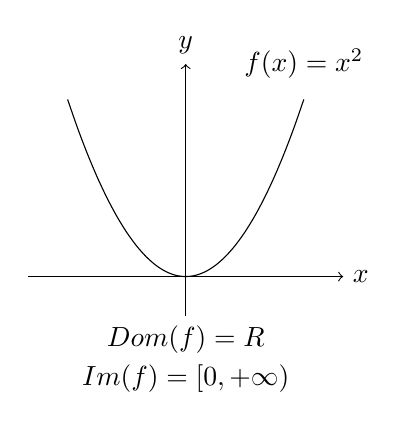
\begin{tikzpicture}
			% f(x) = x^2
			\begin{scope}
				\draw[->] (-2,0) -- (2,0) node[right] {$x$};
				\draw[->] (0,-0.5) -- (0,2.7) node[above] {$y$};
				\draw[domain=-1.5:1.5, smooth, variable=\x] plot ({\x},{\x*\x});
				\node at (1.5,2.7) {$f(x) = x^2$};
				\node[below] at (0,-0.5) {$\text{Dom}(f) = \mathbb{R}$};
				\node[below] at (0,-1) {$\text{Im}(f) = [0, +\infty)$};
			\end{scope}
		\end{tikzpicture}
		\hspace{2cm}
		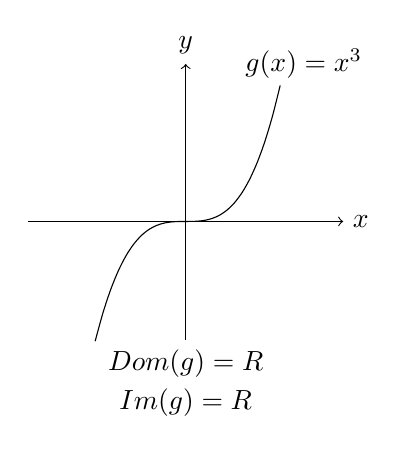
\begin{tikzpicture}
			% g(x) = x^3
			\begin{scope}
				\draw[->] (-2,0) -- (2,0) node[right] {$x$};
				\draw[->] (0,-1.5) -- (0,2) node[above] {$y$};
				\draw[domain=-1.15:1.2, smooth, variable=\x] plot ({\x},{\x*\x*\x});
				\node at (1.5,2) {$g(x) = x^3$};
				\node[below] at (0,-1.5) {$\text{Dom}(g) = \mathbb{R}$};
				\node[below] at (0,-2) {$\text{Im}(g) = \mathbb{R}$};
			\end{scope}
		\end{tikzpicture}
	\end{figure}
\end{example}
\begin{example}
	\(h(x) = \frac{1}{\sqrt{1 - x^{2} } }\)
	
	Dado \(x \in Domh \), se tiene que \(1 - x^{2} \geq 0, \sqrt{1 - x^{2}}  \neq 0 \Rightarrow 1-x^{2}  > 0 \). Por tanto, \(Domh = \set{x \in \R \mid 1 - x^{2} > 0  }\)
	
	Resolviendo la ecuación, obtenemos como raíces \(x = \pm 1 \). Dividiendo por tramos: 
	
	\begin{figure}[H]
		\centering
		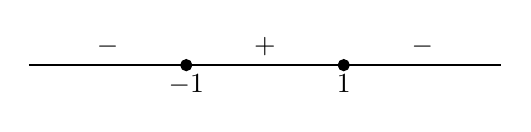
\begin{tikzpicture}
			% Draw the number line
			\draw[thick] (-3,0) -- (3,0);
			
			% Draw the points at -1 and 1
			\filldraw (1,0) circle (2pt);
			\filldraw (-1,0) circle (2pt);
			
			% Draw the labels below the points
			\node[below] at (-1,0) {$-1$};
			\node[below] at (1,0) {$1$};
			
			% Draw the plus and minus signs
			\node[above] at (-2,0) {$-$};
			\node[above] at (0,0) {$+$};
			\node[above] at (2,0) {$-$};
		\end{tikzpicture}
	\end{figure}
	Por lo tanto, \(Domh = (-1,1 )\) ya que es el tramo que cumple que \(1 - x^{2} > 0\). 
	
	Para calcular la imagen de \(h \), sabemos que \( y \in Imh\) si \(\exists x \in (-1,1) \mid h(x) = y\).
	
	\begin{itemize}
		\item Para \(y \leq  0 \): \(\exists x \in (-1,1) \mid h(x) = y \iff 0 < \frac{1}{\sqrt{1 - x^{2} } } = y \leq  0\). No es posible.
		\item Para \(y > 0 \): si \(y \in Imh, \exists x \in (-1,1 )\) tal que \(h(x) = y \Rightarrow \frac{1}{\sqrt{1 - x^{2} } } = y \Rightarrow 1 = y(\sqrt{1 - x^{2} } ) \Rightarrow 1 = y^{2} \cdot (1 - x^{2} ) \Rightarrow \frac{1}{y^{2} } = 1 - x^{2} \Rightarrow x^{2} = 1 - \frac{1}{y^{2} } \Rightarrow x = \pm \sqrt{1 - \frac{1}{y^{2} }}\).
		      
		      Supongamos \(y \in Imh \Rightarrow x \in (-1,1) \mid h(x) = y \Rightarrow \frac{1}{\sqrt{1 - x^{2} } } = y \Rightarrow x = \pm \sqrt{1 - \frac{1}{y^{2} }} {\color{red}\in \R ? } \; 1 - \frac{1}{y^{2} } \geq 0 \iff 1 \geq  \frac{1}{y^{2} } \iff y^{2} \geq 1  \). Luego \(Imh = [1,\infty)\).
		      
		      Cómo comprobamos si \(y \in Imh \)?
		      
		      \(h(\sqrt{1 - \frac{1}{y^{2} }} ) = \frac{1}{\sqrt{1 - (\sqrt{1 - \frac{1}{y^{2} }} )^{2} } } = \frac{1}{\sqrt{1 - 1 + \frac{1}{y^{2} }} } = \frac{1}{\sqrt{\frac{1}{y^{2}}} } = \sqrt{y^{2} } = |y| = y\).
		      
		      Además, \(\sqrt{1 - \frac{1}{y^{2} }} \in (0,1 )\).
		      \begin{itemize}
			      \item \(\sqrt{1 - \frac{1}{y^{2} }} \geq 0 \).
			      \item \(\sqrt{1 - \frac{1}{y^{2} }} < 1 \). \(0 < \frac{1}{y^{2} } \Rightarrow 1 < \frac{1}{y^{2} } + 1 \Rightarrow 1 - \frac{1}{y^{2} } < \frac{1}{y^{2} } + 1 - \frac{1}{y^{2} } \Rightarrow 1 - \frac{1}{y^{2} } < 1 \Rightarrow \sqrt{1 - \frac{1}{y^{2} }} < \sqrt{1} = 1   \)
		      \end{itemize}
	\end{itemize}
\end{example}
\begin{proposition}
	Sea \(f \colon A \to \R \) una funcion y un conjunto \(B \subset A \). Diremos que:
	\begin{itemize}
		\item \(f \) es \textbf{creciente}  en \(B \) si para todo \(x_1,x_2 \in B \), \(x_1 < x_2 \), \(f(x_1) \leq f(x_2 )\).
		\item \(f \) es \textbf{decreciente}  en \(B \) si para todo \(x_1,x_2 \in B ,\) \(x_1,x_2 \in B \), \(x_1 < x_2 \), \(f(x_1) \geq f(x_2 )\).
	\end{itemize}
	Diremos que es estricto cuando aparezca la desigualdad estricta.
\end{proposition}

\begin{proposition}
	Sea \(f \colon A \to \R \) tal que si \(x \in A \), \(-x \in A \). Diremos que:
	\begin{itemize}
		\item \(f \) es \textbf{par}  si \(f(-x) = f(x )\) para todo \(x \in A \)
		\item \(f \) es \textbf{impar}  si \(f(-x) = -f(x )\) para todo \(x \in A \).
	\end{itemize}
\end{proposition}
\begin{definition}
	Sea \(f \colon A \to \R \). Diremos que:
	\begin{itemize}
		\item \(f \) es \textbf{acotada superiormente}  si \(\exists K \in \R \) tal que \(f(x) \leq K \; \forall x \in A \)
		\item \(f \) es \textbf{acotada inferiormente}  si \(\exists K \in \R \) tal que \(f(x) \geq K \; \forall x \in A \)
		\item \(f \) es \textbf{acotada}  si \(\exists K \in \R \) tal que \(|f(x)| \leq K \; \forall x \in A\), o equivalentemente \(\exists K_1,K_2 \in \R \) tal que \(K_2 \leq f(x) \leq K_1 \) (acotada inferior y superiormente).
	\end{itemize}
\end{definition}
\begin{definition}[Composición]
	Sea \(f \colon A \to \R \) y \(g : B \to R \) tal que \(f(a) \subset B \). Se define la función composición como
	\[
		\begin{aligned}
			g \circ f \colon A & \longrightarrow  \R                    \\
			x                  & \longmapsto (g \circ f )(x) = g(f(x))
		\end{aligned}
	\]
\end{definition}
\begin{definition}[Inversa]
	Sea \(f \colon A \to B \). Decimos que \(g \) y \(f \), con \(g \colon B \to A \), son funciones inversas si:
	\[
		(g \circ f)(x) = x \quad \forall x \in A
		\text{ y }
		(f \circ g)(x) = x \quad \forall x \in B \quad (g = f^{-1} )
	\]
\end{definition}

\section{Límites}
\begin{definition}[Límite]
	Diremos que \(\lim\limits_{x \to a} f(x) = l \) si para todo \(\varepsilon > 0 \) existe \(\delta > 0 \) tal que
	\[
		l - \varepsilon < f(x) < l + \varepsilon \text{ cuando } a - \delta < x < a + \delta, \quad x \neq a \;\;(x \text{ es pto. de acumulacion}  ),
	\]
	o también, \(\lim\limits_{x  \to a } f(x) = l \) si \(\forall \varepsilon > 0 \) existe un \(\delta > 0 \) tal que \(|f(x) - l| < \varepsilon \) para todo \(x \in (a - \delta, a + \delta), x \neq a\).
\end{definition}
\begin{example}
	\(\lim\limits_{x  \to 1 } 2x = 2 \).
	
	Cojo un \(\varepsilon > 0 \). Tengo que ver que \(\exists \delta > 0 \) tal que \(|2x - 2| < \varepsilon \; \forall x \in (1-\delta, 1 + \delta), x \neq 1 \Rightarrow \)
	
	\(- \varepsilon < 2x - 2 < \varepsilon \Rightarrow 2 - \varepsilon < 2x < 2 + \varepsilon\).
	
	Luego sabemos que \(2(1-\delta) = 2 - \varepsilon \Rightarrow 1 - \delta = \frac{2 - \varepsilon}{2 } \Rightarrow \delta = 1 - \frac{2-\varepsilon}{2} = 1 -1 + \frac{\varepsilon}{2} = \frac{\varepsilon}{2}\).
	
	Tenemos que dado \(\varepsilon > 0 \), \(\exists \delta = \frac{\varepsilon}{2}\), \(1 - \frac{\varepsilon}{2} < x < 1 + \frac{\varepsilon}{2} \Rightarrow 2 - \varepsilon < 2x < 2 + \varepsilon\).
	
	Hemos encontrado un \(\delta\) que cumple lo anterior. Luego \(\lim\limits_{x  \to a } 2x = 2 \).
\end{example}
\begin{definition}[Límites laterales]
	Sea \(f(x )\) una función definida en \(\R \). 
	
	\begin{itemize}
		\item Diremos que \(\lim\limits_{x  \to \alpha^{+} } f(x) = l  \) es un límite lateral por la derecha si \(\forall \varepsilon > 0 \) \(\; \exists \delta > 0 \) tal que \(\left\vert f(x) - l  \right\vert < \varepsilon \) cuando \(\alpha < x < \alpha + \varepsilon\).
		      
		\item Diremos que \(\lim\limits_{x  \to \alpha^{-} } f(x) = l  \) es un límite lateral por la izquierda si \(\forall \varepsilon > 0 \) \(\; \exists \delta > 0 \) tal que \(\left\vert f(x) - l  \right\vert < \varepsilon \) cuando \(\alpha- \varepsilon < x < \alpha\).
	\end{itemize}
	
\end{definition}
\begin{definition}[Límites infinitos]
	Sea \(f(x )\) una función definida en \(\R \). 
	
	\begin{itemize}
		\item Diremos que \(f(x )\) tiende a infinito en un punto \(\alpha\), \(\lim\limits_{x  \to \alpha} = + \infty \), si \(\forall M \in \R \) \(\; \exists \delta > 0 \) tal que \(f(x) > M \) cuando \(0 < \left\vert x - \alpha \right\vert < \delta\).
		      
		\item Diremos que \(f(x )\) tiende a menos infinito en un punto \(\alpha\), \(\lim\limits_{x  \to \alpha} = - \infty \), si \(\forall m \in \R \) \(\; \exists \delta > 0 \) tal que \(f(x) < m \) cuando \(0 < \left\vert x - \alpha \right\vert < \delta\).
	\end{itemize}
\end{definition}
\begin{definition}[Límites infinitos laterales]
	Sea \(f(x )\) una función definida en \(\R \). 
	
	\begin{itemize}
		\item \(\lim\limits_{x  \to \alpha^{+}} f(x) = +\infty\) si \(\forall M \in \R \; \exists \delta > 0 \) tal que \(f(x) > M \) cuando \(\alpha < x < \alpha + \delta\).
		      
		\item \(\lim\limits_{x  \to \alpha^{-}} f(x) = +\infty\) si \(\forall M \in \R \; \exists \delta > 0 \) tal que \(f(x) > M \) cuando \(\alpha - \delta < x < \alpha\).
	\end{itemize}
	
	Esto es análogo para \(-\infty\), aplicando las definiciones anteriores.   
\end{definition}
\begin{definition}[Límites en el infinito]
	Sea \(f(x )\) una función definida en \(\R \). 
	
	\begin{itemize}
		\item \(\lim\limits_{x  \to +\infty} f(x) = l \in \R \) si \(\forall \varepsilon > 0 \in \R \) \(\; \exists N \in \R \) tal que \(\left\vert f(x) - l  \right\vert < \varepsilon\) cuando \(x > N \).
		\item \(\lim\limits_{x  \to - \infty} f(x) = l \in \R \) si \(\forall \varepsilon > 0 \in \R \) \(\; \exists N \in \R \) tal que \(\left\vert f(x) - l  \right\vert < \varepsilon\) cuando \(x < N \).
	\end{itemize}
\end{definition}


\begin{theorem}[Unicidad del límite]
	Si \(\alpha\) es un punto de acumulacion de \(Domf \) y \(\lim\limits_{x  \to \alpha} f(x )\) existe, entonces es único.
\end{theorem}
\begin{proof}
	Supongamos que \(\lim\limits_{x \to \alpha} f(x) = l_1 \) y \(\lim\limits_{x \to \alpha} = l_2 \), con \(l_1 < l_2 \) (análogo para \(l_2 < l_1\)). Cogemos un \(\varepsilon > 0 \) tal que \((l_1 - \varepsilon, l_1 + \varepsilon) \cap (l_2 - \varepsilon, l_2 + \varepsilon) = \varnothing \Rightarrow l_1 + \varepsilon < l_2 - \varepsilon \Rightarrow 2\varepsilon < l_2 - l_1 \Rightarrow \varepsilon < \frac{l_2 - l_1 }{2}\). 
	
	Como \(\lim\limits_{x  \to \alpha} f(x) = l_1 \Rightarrow  \) para \(\varepsilon > 0 \; \exists \delta_1 > 0 \text{ tal que }  \left\vert f(x) - l_1  \right\vert < \varepsilon \; \forall x \in Domf \cap (\alpha - \delta_1, \alpha + \delta_1 ), x \neq \alpha\). 
	
	Como \(\lim\limits_{x  \to \alpha } f(x) = l_2 \Rightarrow \) para \(\varepsilon > 0 \; \exists \delta_2 > 0 \text{ tal que }  \left\vert f(x) - l_2  \right\vert < \varepsilon \; \forall x \in Domf \cap (\alpha - \delta_2, \alpha + \delta_2 )\), \(x \neq \alpha \).
	
	Defino \(\delta = \min\set{d_1, d_2 }\). Como \(\alpha \) es punto de acumulacion de \(Domf \), \(\exists x_0 \in (\alpha - \delta, \alpha + \delta) \cap Domf \) con \(x_0 \neq \alpha\) que cumple
	\[
		\left\vert f(x_0) - l_1  \right\vert < \varepsilon \Rightarrow - \varepsilon < f(x_0) - l_1 < \varepsilon \Rightarrow l_1 - \varepsilon < f(x_0) < l_1 + \varepsilon
	\]
	y también
	\[
		\left\vert f(x_0) - l_2  \right\vert < \varepsilon \Rightarrow l_2 - \varepsilon < f(x_0) < l_2 + \varepsilon
	\]
	Luego \(f(x_0) \in (l_1 - \varepsilon, l_1 + \varepsilon) \cap (l_2 - \varepsilon, l_2 + \varepsilon)\). Esto es una contradicción con que los intervalos son disjuntos, como habíamos supuesto inicialmente. 
\end{proof}


\begin{proposition}[Criterio de sucesiones]
	\label{caractsuc}
	Sea \(f \colon A \to \R \) y \(\alpha\) un punto de acumulación. Entonces
	\[
		\lim\limits_{x  \to \alpha} f(x) = l \iff (\forall (x_n) \subset A, x_n \overset{n \rightarrow \infty}{\longrightarrow} \alpha, x_n \neq \alpha \Rightarrow f(x_n) \overset{n\rightarrow \infty}{\longrightarrow} l)
	\]
\end{proposition}
\begin{proof}
	\begin{description}
		\item[\(\Rightarrow \)]] Supongamos que \(\lim\limits_{x  \to \alpha} f(x) = l  \). Sea \((x_n )\), \(x_n \overset{n \rightarrow \infty}{\longrightarrow} \alpha \) con \(x_n \neq \alpha\). Tenemos que ver que \(\set{f(x_n )}\) converge a \(l \) \(\Rightarrow \forall \varepsilon > 0 \; \exists n_0 \in \N / \left\vert f(x_n) - l \right\vert < \varepsilon \; \forall n \geq n_0 \).
		
		Sea \(\varepsilon > 0 \). Sabemos que (*) \(\lim\limits_{x  \to \alpha} f(x) = l \), es decir, \(\exists \delta > 0 \) de forma que \(\left\vert f(x) - l  \right\vert < \varepsilon \; \forall x \in A \cap (\alpha - \delta, \alpha + \delta)\), \(x \neq \alpha\).
		
		También sabemos que \(x_n \rightarrow \alpha\), \(x_n \neq \alpha\), luego para \(\delta > 0 \), existe \(n_0 \in \N \) tal que \(\left\vert x_n - \alpha \right\vert < \delta \; \forall n \geq n_0\). Entonces, por (*) tenemos que \(\left\vert f(x_n) - l  \right\vert < \varepsilon \; \forall n \geq n_0\) ya que \(x_n \in A \), \(\left\vert x_n - \alpha \right\vert < \delta\). Por tanto, \(\lim\limits_{n  \to \infty} f(x_n) = l\). 
		
		\item[\(\Leftarrow \)]] Supongamos que no existe \(\lim\limits_{x \to \alpha} f(x)\) y veamos que esto implica lo contrario de la hipótesis, es decir, que \(\exists \set{x_n } \subset A, x_n \rightarrow \alpha, x_n \neq \alpha\) tal que \(f(x_n) \cancel \rightarrow l \).
		
		Si \(\cancel \exists \lim\limits_{x  \to \alpha} f(x) = l , \exists \varepsilon > 0  \) tal que \(\forall \delta > 0 \; \exists x \in A \cap (\alpha - \delta, \alpha + \delta), x \neq \alpha,\) tal que \(\left\vert f(x) - l \right\vert \geq \varepsilon\). Elegimos \(\delta = \frac{1}{n }\) con \(n \in \N  \Rightarrow \exists x_n \in A \cap (\alpha - \delta, \alpha + \delta)\) tal que \(\left\vert f(x_n) - l  \right\vert \geq \varepsilon\). Entonces \(x_n \in (\alpha - \frac{1}{n}, \alpha + \frac{1}{n}) \Rightarrow x_n \rightarrow \alpha\). Tambien tenemos que \(\left\vert f(x_n) - l  \right\vert \geq \varepsilon\), luego \(f(x_n) \cancel \rightarrow l \).
	\end{description}
\end{proof}

\vspace{0.2cm}
\begin{proposition}
	Supongamos que \(\lim\limits_{x  \to \alpha} f(x) = l \) y \(\lim\limits_{x  \to \alpha} g(x) = m \), entonces
	\begin{itemize}
		\item \(\lim\limits_{x  \to \alpha} f(x) + g(x) = l + m \)
		\item \(\lim\limits_{x \to \alpha} \lambda f(x) = \lambda \cdot l, \lambda \in \R \)
		\item \(\lim\limits_{x  \to \alpha} f(x) g(x) = l \cdot m \)
		\item \(\lim\limits_{x  \to \alpha} \frac{f(x )}{g(x )} = \frac{l }{m }\)
		\item \(\lim\limits_{x  \to \alpha} f(x)^{g(x)} = l^{m} \)
	\end{itemize}
\end{proposition}
\begin{proof}
	Probaremos el primer resultado utilizando la definición de límite.
	\begin{itemize}
		\item Tenemos que probar que, dado \(\varepsilon > 0, \exists \delta > 0 \) tal que \(\left\vert f(x) + g(x) - (l + m ) \right\vert < \varepsilon \; \forall x \in Dom(f + g) \cap (\alpha - \delta, \alpha + \delta)\) con \( x \neq \alpha \).
		      
		      Sea \(\frac{\varepsilon}{2} > 0 \). Sabemos que \(\exists \delta_1 > 0 / \left\vert f(x) - l  \right\vert < \frac{\varepsilon}{2} \; \forall x \in Domf \cap (\alpha - \delta_1, \alpha + \delta_1) \). Tambien \(\exists  \delta_2 > 0 / \left\vert g(x) - m  \right\vert < \frac{\varepsilon}{2} \; \forall x \in Domg \cap (\alpha - \delta_2, \alpha + \delta_2)\).
		      
		      Definimos \(\delta = \min \set{\delta_1,\delta_2} > 0 \) y entonces se tiene que, \(\forall x \in Dom(f + g) \cap (a - \delta, a + \delta)\),  
		      \begin{multline*}
			      \left\vert f(x) + g(x) - (l + m ) \right\vert = \left\vert f(x) - l + g(x) - m  \right\vert \leq \left\vert f(x) - l  \right\vert + \left\vert g(x )  - m \right\vert < \frac{\varepsilon}{2} + \frac{\varepsilon}{2} = \varepsilon
		      \end{multline*}
	\end{itemize}
	Todas las propiedades se pueden demostrar o bien de este modo o bien por sucesiones, aplicando la caracterización \ref{caractsuc}. Probaremos también la propiedad del límite del producto de funciones siguiendo el segundo método: 
	\begin{itemize}
		\item Sea \((x_n )\) cualquier sucesión en \(A \) tal que \(x_n \neq \alpha \; \forall n \in \N\) y \( \lim\limits_{n \to \infty} x_n = \alpha\). Por el teorema \ref{caractsuc} se obtiene que \(\lim\limits_{n \to \infty} f(x_n) = l \) y \(\lim\limits_{n \to \infty} g(x_n) = m\).
		      
		      Por lo tanto, aplicando las propiedades de límites de sucesiones (\ref{proplimsuc}), llegamos a que 
		      \[
			      \lim\limits_{n \to \infty} f(x_n) g(x_n) = (\lim\limits_{n \to \infty} f(x_n)) (\lim\limits_{n \to \infty} g(x_n)) = l \cdot m.
		      \]
		      Luego, aplicando de nuevo el teorema \ref{caractsuc}, 
		      \[
			      \lim\limits_{x  \to \alpha} f(x)g(x ) = \lim\limits_{n \to \infty} f(x_n) g(x_n) = l \cdot m. 
		      \]
	\end{itemize}
\end{proof}
\begin{proposition}
	Supongamos que \(\lim\limits_{x  \to \alpha} f(x) = l \) y \(\lim\limits_{y  \to l} h(y) =m  \), entonces \(\lim\limits_{x  \to \alpha} h(f(x)) = m \).
\end{proposition}
% \begin{example}
% 	\begin{itemize}
% 		\item \(\lim\limits_{x  \to \infty } (\frac{2x + 7 }{2x - 6 })^{\sqrt{4x^{2}  + x - 3 } } = (1^{\infty} ) \)

% 		      \(\lim\limits_{x  \to \infty} \frac{2x + 7 }{2x - 6 } \overset{\frac{\infty}{\infty}}{=} \lim\limits_{x  \to \infty} \frac{2 + \frac{1}{x}}{2 - \frac{6}{x}} = 1\).

% 		      \(\lim\limits_{x  \to \infty} ^{4x^{2} + x - 3 } =  \infty\)

% 		      \(\lim\limits_{x  \to \infty } (\frac{2x + 7 }{2x - 6 })^{\sqrt{4x^{2}  + x - 3 } } = \lim\limits_{x  \to \infty} \sqrt{4x^{2} + x - 3  }(\frac{2x + 7 - 2x + 6 }{2x - 6})  = \lim\limits_{x  \to \infty} \sqrt{4x^{2} + x -3 } \cdot \frac{13}{2x - 6} = 13 \lim\limits_{x  \to \infty} \frac{\sqrt{4x^{2} + x - 3 } }{2x - 6}  \overset{\frac{\infty}{\infty}}{=} 13 \lim\limits_{x  \to \infty} \frac{\frac{\sqrt{4x^{2} } }{}}{}\)
% 	\end{itemize}
% \end{example}

\begin{proposition}[Regla del sandwich]
	Sea \(A \subseteq R \), sean \(f,g,h \colon A \to \R \) y sea \(c \in \R \) un punto de acumulacion de \(A \). Si
	\[
		f(x) \leq g(x) \leq h(x) \quad \text{ para toda }\quad x \in A, x \neq c,
	\]
	y si \(\lim\limits_{x  \to c } f = L = \lim\limits_{x  \to c } h \), entonces \(\lim\limits_{x  \to c } g = L \).
\end{proposition}

\begin{example}
	\begin{itemize}
		\item \(\lim\limits_{x  \to \infty} e^{-x}senx  \).
		      
		      Sabemos que \(-1 \leq \sin x \leq 1 \; \forall x \in \R \Rightarrow - e^{-x} \leq e^{-x} \sin x \leq e^{-x}   \).
		      
		      Como \((-1)e^{-x} \overset{x\to \infty}{\longrightarrow } 0 \) y  \(e^{-x} \overset{x\to \infty}{\longrightarrow } 0 \), aplicando la regla del sandwich, \(\lim\limits_{x  \to \infty} e^{-x}senx  = 0\).
		      
		\item \(\lim\limits_{x  \to 0} x \cos \frac{1}{x }\). Sabemos que \(-1 \leq \cos \frac{1}{x} \leq  1 \;\forall x \in \R \setminus \set{0 }\).
		      
		      \(\lim\limits_{x  \to 0^{+}  } x \cos \frac{1}{x}\): \(-1 \leq \cos \frac{1}{x} \leq  1 \Rightarrow -x (\rightarrow 0)\leq x \cdot \cos \frac{1}{x} \leq x (\rightarrow 0)\). Por tanto, \(\lim\limits_{x \to 0^{+} } x \cos \frac{1}{x} = 0 \).
		      
		      \(\lim\limits_{x \to 0^{-} } x \cos  \frac{1}{x} \): \(-1 \leq \cos \frac{1}{x} \leq 1 \Rightarrow -x (\rightarrow 0)\geq x\cos  \frac{1}{x} \geq x (\rightarrow 0)\). Luego \(\lim\limits_{x  \to 0^{-} } x \cos \frac{1}{x} = 0 \).
		      
		      Entonces \(\lim\limits_{x  \to 0 } x \cos \frac{1}{x} = 0 . \)
		      
		      Otra forma es considerar el valor absoluto: \(\lim\limits_{x  \to 0 } \left\vert x \cos \frac{1}{x } \right\vert = \lim\limits_{x  \to 0 } \left\vert x 	\right\vert \left\vert \cos  \frac{1}{x } \right\vert \)
		      
		      \(0 \leq \left\vert \cos \frac{1}{x } \right\vert \leq 1 \Rightarrow 0 \leq \left\vert x  \right\vert \left\vert \cos  \frac{1}{x } \right\vert \leq \left\vert x  \right\vert \). Como \(0 \rightarrow 0 \) y \(\left\vert x  \right\vert \rightarrow 0 \), \(\lim\limits_{x  \to 0 } \left\vert x \cos  \frac{1}{x } \right\vert= 0 \).
	\end{itemize}
\end{example}
\begin{proposition}
	\label{limitepositivo}
	Sea \(A \subseteq \R \), sea \(f \colon A \to \R\) y sea \(c \in \R \) un punto de acumulación de \(A \). Si 
	\(
	\lim\limits_{x  \to c } f(x) > 0
	\), 
	entonces \(\exists \delta > 0 \) tal que si \(x \in (c - \delta, c + \delta), x \neq c \), \(f(x) > 0\).\footnote{También se puede demostrar que si el límite es negativo la función es negativa alrededor (similar).}
\end{proposition}
\begin{proof}
	Supongamos que \(\lim\limits_{x  \to c } f(x) = l \), con \(l >0 \). Tomamos \(\epsilon = \frac{1}{2} l > 0 \) y, aplicando la definición de límite, se tiene que \(\exists \delta > 0 \) tal que si \(0 < \left\vert x - c  \right\vert < \delta\) y \(x \in A \), entonces \(\left\vert f(x) - l  \right\vert < \frac{1}{2} l\). Luego \(-\frac{1}{2}l < f(x) - l < \frac{1}{2} l \Rightarrow \frac{1}{2} l < f(x) < \frac{3}{2} l\). En particular, \(f(x) > \frac{1}{2} l > 0\).        
\end{proof}
\section{Continuidad}
\begin{definition}
	Diremos que una función \(f \) es continua en \(x_0 \in Domf\), con \(x_0 \) un punto de acumulación, si y sólo si \(\lim\limits_{x  \to x_0 } f(x)= f(x_0 )\).
	
	Diremos que \(f \) es continua en un intervalo \((a,b )\) si es continua en todos los puntos. De igual forma, diremos que \(f \) es continua en \([a,b ]\) si es continua en \((a,b )\) y continua por la derecha de \(a \) y por la izquierda de \(b \).
\end{definition}
\begin{example}
	Funciones continuas en su dominio son: polinomios, \(\sin x\), \(\cos x\), \(\sqrt{x }\), \(e^{x}\), \(\ln x, \ldots\)     
\end{example}
Además, sumar o multiplicar dos funciones continuas, dividir dos funciones continuas con denominador distinto de cero, composicion de funciones continuas, es una función continua.
\begin{definition}[General de continuidad]
	Sea \(A \subset \R \), \(f\colon A \to \R \) y \(x_0 \in A \), se dice que \(f \) es continua en \(x_0 \) si \(\forall \varepsilon > 0 \) \(\exists \delta > 0 \) tal que \(\forall x \in (x_0 - \delta, x_0 + \delta) \cap A\) se cumple que
	\[
		\left\vert f(x) - f(x_0 ) \right\vert < \varepsilon.
	\]
\end{definition}

% \begin{remark}
% 	Si \(x_0 \) es punto de acumulacion de \(A \),
% 	\[
% 		f \text{ es continua en } x_0 \iff \lim\limits_{x  \to x_0 } f(x) = f(x_0)
% 	\]
% \end{remark}
\begin{theorem}
	Sea \(A \subseteq \R \), \(\alpha_0 \in A \). Entonces
	\[
		f \text{ es continua en } x_0 \iff (\forall \set{x_n} \subset A, x_n \longrightarrow x_0 \Rightarrow f(x_n) \rightarrow f(x_0))
	\]
\end{theorem}
\section{Teoremas sobre funciones continuas}
\begin{theorem}[de Bolzano]
	Sean \(a,b \in \R \) con \(a < b \) y supongamos que \(f \colon A \to \R \) es continua en \([a,b] \subset A \). Si se cumple que
	\[
		\text{signo}(f(a)) \neq \text{signo}(f(b)) \text{ con } f(a) \neq 0 \text{ y } f(b) \neq 0
	\]
	entonces existe \(c \in (a,b )\) tal que \(f(c) = 0 \).
\end{theorem}
\begin{proof}
	Supongamos que \(f(a) > 0 \) y \(f(b) < 0\). Consideramos \(\gamma = \frac{a + b}{2}\). Hay tres casos:
	\begin{itemize}
		\item \(f(\gamma) = 0\). Entonces \(c = \gamma\) y queda demostrado.
		\item \(f(\gamma) < 0 \). Defino \(a_1 = a \) y \(b_1 = \gamma\). Entonces \(f(a_1) >0 \) y \(f(b_1) < 0 \) y se puede repetir el proceso. Definimos \(\gamma = \frac{a_1 + b_1 }{2 }\). Puede ocurrir que \(f(\gamma) = 0, f(\gamma) > 0 \) o \(f(\gamma) < 0 \). Si \(f(\gamma) = 0, c = \frac{a_1 + b_1}{2}\). Si \(f(\gamma) > 0 \), definimos \(a_2 = \frac{a_1 + b_1 }{2 }\) y \(b_2 = b_1\). Si \(f(\gamma) < 0 \), defino \(a_2 = a_1 \) y \(b_2 = \frac{a_1 + b_1 }{2 }\). Si sigo repitiendo el proceso, obtengo que dado \(I_n = [a_n,b_n], f(a_n) > 0 \), \(f(b_n) < 0 \), \(I_{n+1} \subset I_n \). Por el teorema de los intervalos anidados (\ref{anidados}), si \(I_n = [a_n,b_n ]\) cumple que \(I_n \supset I_{n+1} \; \forall n \in \N \), entonces \(\exists c \in \R \) tal que \(c \in I_n \; \forall  n \in \N \). Falta demostrar que \(c \) es el punto tal que \(f(c) = 0\).
		      
		      Sabemos que \(b_1 - a_1 = \frac{b - a }{2}, b_2 - a_2 = \frac{b - a }{4} = \frac{b - a }{2^{2} }\). En general, \(b_n - a_n = \frac{b - a }{2^{n} }\).
		      
		      Como \(c \in I_n \;\forall n \in \N \),
		      \begin{itemize}
			      \item \(a_n \leq c \leq b_n \Rightarrow a_n - a_n \leq c - a_n \leq b_n - a_n \Rightarrow 0(\rightarrow 0) \leq c - a_n \leq b_n - a_n = \frac{b - a }{2^{n} }(\rightarrow 0)\). Luego, por el teorema del sandwich, \(\lim\limits_{n \to \infty} c - a_n = 0 \).
			            
			            Por tanto, \(\lim\limits_{n \to \infty} a_n = \lim\limits_{n \to \infty} c - c + a_n = \lim\limits_{n \to \infty} c - \lim\limits_{n \to \infty} c - a_n = c - 0 = c \) y \(\lim\limits_{n \to \infty} a_n = c \).
			      \item Siguiendo el mismo razonamiento, también se tiene que \(\lim\limits_{n \to \infty} b_n = c \).
		      \end{itemize}
		      Como \(f \) es continua en \([a,b] \subset A \), si \(a_n \rightarrow c \) entonces \(f(a_n) \rightarrow f(c )\) y si \(b_n \rightarrow c \) entonces \(f(b_n) \rightarrow f(c )\).
		      
		      Además, \(f(a_n) \geq 0 \; \forall n \) y \(f(b_n ) \leq 0 \;\forall n \). Por tanto, la única opción es que \(f(c) = 0 \).
		\item \(f(\gamma ) > 0 \). Llamamos \(a_1 = \frac{a+ b }{2} \) y \(b_1 = b \Rightarrow f(a_1) > 0\) y \(f(b_1) < 0 \). El proceso es análogo al de cuando \(f(\lambda) < 0 \).
	\end{itemize}
\end{proof}

\begin{example}
	\begin{itemize}
		\item \(\exists x \in \R \text{ tal que } \cos (x ) = x \)?
		      
		      \(f(x) = \cos x - x \in C(\R )\) (continua). Se tiene que
		      \(F(0) = \cos 0  - 0 = 1 > 0\) y \(F(\frac{\pi}{2}) = \cos \frac{\pi}{2} - \frac{\pi}{2} = - \frac{\pi}{2} < 0 \). Por el teorema de Bolzano, sabemos que \(\exists c \in (0, \frac{\pi}{2})\) tal que \(F(c) = 0 \Rightarrow \cos c - c = 0 \Rightarrow \cos  c = c \).
		      
	\end{itemize}
\end{example}
\begin{example}
	\begin{itemize}
		\item Ejercicio 5 pg 147 - Sea que \(f,g \) esten definidas en \(A \subseteq \R \) a \(\R \) y sea \(c \) punto de acumulacion de \(A \). Supongase que \(f \) esta acotada en una vecindad de \(c \) y que \(\lim\limits_{x  \to c } g = 0 \). Demostrar que \(\lim\limits_{x  \to  c } fg = 0 \).
		      
		      Es decir, que para \(\forall \varepsilon > 0, \text{tomando } \frac{\varepsilon}{M},  \;\exists \delta > 0\) tal que \(\forall x \in (c - \delta, c + \delta) \cap A \), \(\left\vert f(x)g(x) - 0  \right\vert < \frac{\varepsilon}{M}\).
		      
		      Sabemos que \(f \) esta acotada alrededor de \(c \), es decir, existe \(M > 0 \), \(\exists \hat{\delta} > 0 \), \(\left\vert f(x ) \right\vert < M \; \forall x \in (c - \hat{\delta}, c + \hat{\delta })\).
		      
		      Por otro lado, sea \(\varepsilon > 0 \). Sabemos que \(\lim\limits_{x  \to c } g = 0 \), entonces para \(\frac{\varepsilon}{M}\) \(\exists \overline{\delta} > 0 \) tal que \(\forall x \in (c - \overline{\delta}, c + \overline{\delta}) \cap A, \left\vert g(x) - 0  \right\vert < \frac{\varepsilon}{M}\).
		      
		      Si tomamos \(\delta = \min\set{\overline{\delta}, \hat{\delta }}\). Tengo que probar que \(\forall x \in (c - \delta, c + \delta) \cap A, x \neq c \), se cumple \(\left\vert f(x) g(x) - 0  \right\vert < \varepsilon\). Luego
		      \[
			      \left\vert f(x)g(x) - 0  \right\vert = \left\vert f(x) g(x ) \right\vert  = \left\vert f(x ) \right\vert \cdot \left\vert g(x ) \right\vert < M \cdot \frac{\varepsilon}{M} = \varepsilon
		      \]
		      % \item Ejercicio 9 pg 147. Sea que \(f,g \) esten definidas de \(A \) en \(\R \) y sea \(c \) un punto de acumulacion de \(A \).
		      %       \begin{enumerate}
		      % 	      \item[a)] Demostrar que si existe tanto \(\lim\limits_{x  \to c } f \) como \(\lim\limits_{x  \to c } (f+g) \), entonces existe \(\lim\limits_{x  \to c } g .\)
		      
		      % 		      Utilizando las propiedades de los límites, \(\lim\limits_{x  \to c } g = \lim\limits_{x  \to c } g + f - f = \lim\limits_{x  \to c } g + f - \lim\limits_{x \to c} f \). Como es la resta de dos límites que existen, entonces \(\lim\limits_{x  \to c } g \) existe.
		      
		      % 	      \item[b)] Si existen \(\lim\limits_{x  \to c } f \) y \(\lim\limits_{x  \to c } fg \), se sigue que existe \(\lim\limits_{x  \to c } g \)?
		      
		      % 		      Falso. Contraejemplo: \(\lim\limits_{x  \to 0 } x = 0 \) y \(\lim\limits_{x  \to 0 } x \sin \frac{1}{x} = 0 \). Pero \(\lim\limits_{x  \to 0 } \sin \frac{1}{x}\) no existe.
		      %   \end{enumerate}
	\end{itemize}
\end{example}
\begin{theorem}
	Sean \(A,B \subseteq \R \) y sean \(f \colon A \to \R\) y \(g \colon B \to \R\) funciones tales que \(f(A) \subseteq B\). Si \(f \) es continua en un punto \(c \in A \) y \(g \) es continua en \(b = f(c ) \in B\), entonces la composición \(g \circ f\colon A \to \R\) es continua en \(c \).       
\end{theorem}
\begin{proof}
	Sea \(W \) una vecindad de \(g(b )\). Puesto que \(g \) es continua en \(b \), existe una vecindad \(V \) de \(b = f(c )\) tal que si \(y \in B \cap V\) entonces \(g(y) \in W \). Puesto que \(f \) es continua en \(c \), existe una vecindad \(U \) de \(c \) tal que si \(x \in A \cap U\), entonces \(f(x) \in V\). Puesto que \(f(A) \subseteq B\), se sigue que si \(x \in A \cap U \), entonces \(f(x) \in B \cap V \), de modo que \((g \circ  f)(x) = g(f(x)) \in W\). Pero como \(W \) es una vecindad cualquiera de \(g(b )\), esto indica que \(g \circ  f\) es continua en \(c \).          
\end{proof}
\begin{theorem}[Teorema de Darboux]
	Sean \(a,b \in \R \) con \(a < b \) y supongamos que \(f\colon A \to \R \) es continua en \([a,b] \subset A \).
	
	\begin{itemize}
		\item Si \(f(a) < f(b )\), entonces para cada \(z \in (f(a), f(b ))\), existe \(c \in (a,b )\) tal que
		      \[
			      f(c) = z
		      \]
		\item Si \(f(a) > f(b)\) entonces para cada \(z \in (f(b), f(a ))\), existe \(c \in (a,b )\) tal que
		      \[
			      f(c) = z
		      \]
	\end{itemize}
\end{theorem}
\begin{proof}
	No vista en clase. 
\end{proof}

\begin{theorem}[Teorema de Weierstrass]
	Sean \(a,b \in \R \) con \(a < b \) y supongamos que \(f \colon A \to B \) es continua en \([a,b] \subset A \).
	
	Entonces:
	\[
		f \text{ esta acotada en }[a,b]
	\]
	Ademas, existen \(x_m, x_M \in [a,b ]\) tales que
	\[
		f(x_m) \leq f(x) \leq f(x_M) \; \forall x \in [a,b ]
	\]
\end{theorem}
\begin{proof}
	No vista en clase. 
\end{proof}

\part{Derivadas}
\section{¿Qué es la derivada?}
\begin{definition}[Derivada]
	Se define la derivada de \(f \) en el punto \(x_0 \in I \subset Domf \) como:
	\[
		f^\prime (x_0) = \lim\limits_{h  \to 0 } \frac{f(x_0 + h ) - f(x_0)}{h} = \lim\limits_{x  \to x_0 } \frac{f(x) - f(x_0)}{x - x_0}
	\]
	Decimos que \(f \) es derivable en \(x_0 \) si su derivada existe y es finita.
\end{definition}
Notacion: \(f^\prime (x_0) = \frac{df}{dx} (x_0) = \frac{df(x)}{dx}|_{x = x_0} = \frac{df}{dx}|_{x = x_0}\).

\begin{definition}
	Decimos que \(f \) es derivable en un intervalo \((a,b )\) si es derivable en cada punto del intervalo.
\end{definition}

Supongamos que \(f \) es derivable en \(x_0 \) y construyamos la recta tangente de \(f \) en \(x_0 \).

Sabemos que cualquier recta es de la forma: \(y = m(x-x_0) + b \) donde \(m,b \in \R \) estan sin determinar. Además, cualquier recta que pase por \((x_0, f(x_0 ))\) cumple \(f(x_0) = m(x_0 - x_0) + b \rightarrow b = f(x_0 )\).

Ahora, la recta que pasa también por \((x_0 + h, f(x_0 + h ))\) tiene pendiente: \(y = m_h(x - x_0) + f(x_0 )\Rightarrow f(x_0 + h) = m_h (x_0 + h - x_0) + f(x_0) \Rightarrow m_h = \frac{f(x_0 + h) - f(x_0)}{h}\). Por tanto, cuando \(h \to 0\),
\[
	y = \frac{f(x_0 + h) - f(x_0)}{h} (x - x_0) + f(x_0) \Rightarrow \boxed{y = f^\prime (x_0) (x - x_0) + f(x_0)}
\]

\begin{definition}[Derivadas laterales]
	Podemos hablar de derivadas laterales de \(f \) en \(x_0 \) calculando los límites laterales:
	\[
		f^\prime_+(x_0) = \lim\limits_{h  \to 0^{+ } } \frac{f(x_0 + h) - f(x_0)}{h } \text{ y } f^\prime_-(x_0) = \lim\limits_{h  \to 0^{- } } \frac{f(x_0 + h) - f(x_0)}{h }
	\]
	E igualmente, decimos que es derivable por la derecha o por la izquierda si el límite correspondiente es finito y existe. Ademas, \(f \) es derivable en un intervalo \([a,b ]\) si es derivable en \((a,b )\), derivable por la derecha de \(a \) y derivable por la izquierda de \(b \), del mismo modo para el resto de intervalos.
\end{definition}
% \begin{remark}
% 	\begin{itemize}
% 		\item Si existen \(f^\prime_+(x_0 )\) y \(f^\prime_-(x_0 )\) y son iguales, entonces existe \(f^\prime (x_0 )\) y cumple \(f^\prime (x_0) = f^\prime_+(x_0) = f^\prime_-(x_0 )\) 
% 		\item Si existe \(f^\prime (x_0 )\), entonces existen \(f^\prime_+(x_0)\) 
% 	\end{itemize}
% \end{remark}

\section{Fórmulas de las derivadas}
Todas las formulas que nos han enseñado en bachillerato son demostradas utilizando la definición de límite. Por ejemplo,
\[
	f(x) = \sqrt{x} \Rightarrow f^\prime (x) = \frac{1}{2 \sqrt{x } }
\]
\begin{proof}
	Si \(x_0 > 0 \),
	\begin{align*}
		\lim\limits_{h  \to 0} \frac{f(x_0 + h) - f(x_0) }{h} & = \lim\limits_{h  \to 0 } \frac{\sqrt{x_0 + h} - \sqrt{x_0}  }{h} = \lim\limits_{h  \to 0 } \frac{x_0 + h - x_0}{h (\sqrt{x_0 + h} + \sqrt{x_0}  )} \\ & = \lim\limits_{h  \to 0 } \frac{1 }{\sqrt{x_0 + h } + \sqrt{x_0 } } = \frac{1}{2 \sqrt{x_0 } }
	\end{align*}
\end{proof}

Y en \(x_0 = 0\)? \(f^\prime (0 )\) no tiene sentido porque \(f \) no esta definida en un entorno de \(0 \). Y habrá fórmula para la derivada por la derecha en \(x_0 = 0 \)?
\[
	\lim\limits_{h  \to 0^{+} } \frac{f(0 + h ) - f(0)}{h} = \lim\limits_{h  \to 0^{+} } \frac{\sqrt{h } }{h } = \lim\limits_{h  \to 0^{+ } } \frac{1}{\sqrt{h} } = \infty \Rightarrow \text{ No es derivable por la derecha en }0.
\]

Cuándo puedo utilizar las fórmulas de las derivadas en \(x_0\)?
\begin{itemize}
	\item \(x_0 \in Domf \).
	      
	      \(f(x) = \ln x \Rightarrow f^\prime (x) = \frac{1}{x}\) solamente es valida en \((0,\infty )\).
	      
	\item La fórmula tiene que tener sentido.
	      \[
		      f(x) = arcsen(x) \Rightarrow f^\prime (x) = \frac{1}{\sqrt{1 - x^{2} } } \text{ solamente es valida en } (-1,1).
	      \]
	      \[
		      f(x) = \sqrt[3]{x} \Rightarrow f^\prime (x) = \frac{1}{3 \sqrt[3]{x^{2} } } \text{ solamente es valida en } \R \setminus \set{0}
	      \]
	\item \(f(x )\) tiene que tener la misma expresión en un entorno de \(x_0 \).
	      \[
		      f(x) = \begin{cases}
			      x^{2} \text{ si } x \leq 2 \\
			      x \text{ si } x > 2
		      \end{cases} \Rightarrow f^\prime (x) = \begin{cases}
			      2x \text{ si } x < 2 \\
			      ? \text{ si } x = 2  \\
			      1 \text{ si } x < 2
		      \end{cases}
	      \]
	      Sin embargo, para calcular \(f^\prime (2 )\) habría que calcularlo de otra forma.
	      
	      \[
		      f^\prime (2) = \lim\limits_{h  \to 0 } \frac{f(2 + h) - f(2)}{h } = \lim\limits_{h  \to 0 } \frac{f(2 + h) - 4 }{h }
	      \].
	      
	      Calculamos los límites laterales:
	      \[
		      \begin{dcases}
			      \lim\limits_{h  \to 0^{-}  } \frac{(2 + h)^{2} - 4 }{h} = \lim\limits_{h  \to 0^{- } } \frac{4 + h^{2} - 4h - 4 }{h} = \lim\limits_{h  \to 0^{-}  } \frac{4 + h^{2} + 4h - 4}{h} = \lim\limits_{h  \to 0^{-} } h + 4 = 4 \\
			      \lim\limits_{h  \to 0^{+}  } \frac{2 + h - 4}{h } = \lim\limits_{h  \to 0^{+} } \frac{h - 2}{h } = \frac{-2}{0^{+} } = -\infty
		      \end{dcases}
	      \]
	      Como no coinciden, la funcion no es derivable en \(2\).
\end{itemize}
\section{Propiedades de las derivadas}
\begin{proposition}
	Sean \(f \) y \(g \) derivables en \(x_0 \) y \(\lambda \in \R \), entonces:
	\begin{itemize}
		\item \(f +g \) es derivable en \(x_0 \) y \((f + g)^\prime (x_0) = f^\prime (x_0) + g^\prime (x_0 )\).
		\item \(\lambda f \) es derivable en \(x_0 \) y \((\lambda f)^\prime (x_0) = \lambda f^\prime (x_0)\).
		\item \(f \cdot g \) es derivable en \(x_0 \) y \((f \cdot g)^\prime (x_0) = f^\prime (x_0) g (x_0) + f(x_0) g^\prime (x_0 )\)
		\item Si \(g(x_0) \neq 0, \frac{f}{g}\) es derivable en \(x_0 \) y \((\frac{f}{g}) (x_0) = \frac{f^\prime (x_0) g(x_0) - f(x_0) g^\prime (x_0)}{g^{2}(x_0) }\).
	\end{itemize}
\end{proposition}
\begin{proof}
	\begin{itemize}
		\item
		      \begin{align*}
			      (f + g)^\prime (x_0) & = \lim\limits_{h  \to 0 } \frac{(f + g)(x_{0} + h) - (f + g)(x_0)}{h} \\&  =  \lim\limits_{h  \to 0 } \frac{f(x_0 + h) + g(x_0 + h) - (f(x_0) + g(x_0))}{h } \\ &  = \lim\limits_{h  \to 0 } \frac{f(x_0 + h) - f(x_0)}{h} + \lim\limits_{h  \to 0 } \frac{g(x_0 + h) - g(h)}{h } \\ & = f^\prime (x_0) + g^\prime (x_0)
		      \end{align*}
		      Como \(f,g \) son derivables en \(x_0 \Rightarrow f^\prime (x_0), g^\prime (x_0) \in \R \Rightarrow (f + g)^\prime (x_0) = f^\prime (x_0) + g^\prime (x_0) \in \R \) y \(f + g \) es derivable.
		\item  
		      \begin{align*}
			      (\lambda f)^\prime (x_0) & = \lim\limits_{h  \to 0 } \frac{(\lambda f)(x_0 + h) - (\lambda f)(x_0)}{h} = \lim\limits_{h  \to 0 } \frac{\lambda f(x_{0} + h ) - \lambda f(x_0)}{h} \\ & = \lim\limits_{h  \to 0 }\lambda \cdot \frac{f(x_0 + h) - f(x_0)}{h} = \lim\limits_{h  \to 0 } \lambda \cdot \lim\limits_{h  \to 0} \frac{f(x_0 + h) - f(x_0)}{h} \\ & = \lambda f^\prime (x_0)
		      \end{align*}
		\item \begin{multline*}
			      (f \cdot g)^\prime (x_0) = \lim\limits_{h  \to 0 } \frac{(f \cdot g)(x_0 + h) - (f \cdot g)(x_0)}{h} = \lim\limits_{h  \to 0 } \frac{f(x_0)g(x_0 + h) - f(x_0)g(x_0)}{h} = \\ = \lim\limits_{h  \to 0 } \frac{f(x_0 + h)g(x_0 + h) - f(x_0) \cdot g(x_0 + h) + f(x_0)g(x_0 + h) - f(x_0)g(x_0)}{h} = \\ = \lim\limits_{h  \to 0 } \frac{g(x_0 + h) (f(x_0 + h) - f(x_0))}{h} + \lim\limits_{h  \to 0 } \frac{f(x_0) \cdot (g(x_0 + h) - g(x_0))}{h} = \\ =  \lim\limits_{h  \to 0 } g(x_0 + h) \cdot \lim\limits_{h   \to 0 } \frac{f(x_0 + h) - f(x_0)}{h} + g(x_0) \cdot \lim\limits_{h  \to 0 } \frac{g(x_0 + h) - g(x_0)}{h } = \\ = f^\prime(x_0) \cdot \lim\limits_{h  \to 0 } g(x_0 + h ) + f(x_0) \cdot g^\prime (x_0) \overset{g\text{ continua en } x_0 }{= } f^\prime (x_0) g(x_0) + f(x_0) g^\prime (x_0)
		      \end{multline*}
		\item Añadir.
	\end{itemize}
\end{proof}
\begin{theorem}
	Sea \(f \colon I \to \R \) con \(I = (a,b)\).
	Si \(f \) es derivable en \(x_0\), entonces \(f \) es continua en \(x_0 \).
\end{theorem}
\begin{proof}
	Dado \(x \in I \), \(x \neq x_0\), 
	\[
		f(x) - f(x_0) = \frac{(f(x) - f(x_0))}{x - x_0} (x - x_0)
	\]
	Además, tenemos que
	\[
		\lim\limits_{x  \to x_0 } f(x) - f(x_0) = \lim\limits_{x  \to x_0 } \frac{f(x) - f(x_0)}{x - x_0} \cdot \lim\limits_{x  \to x_0 } x - x_0 = f^\prime (x_0) \cdot 0 = 0
	\]
	Por tanto, \(\lim\limits_{x  \to x_0 } (f(x) - f(x_0)) = 0 \).
	\[
		\lim\limits_{x  \to x_0 } f(x) = \lim\limits_{x  \to x_0 } (f(x) - f(x_0) + f(x_0)) = \lim\limits_{x  \to x_0 } (f(x) - f(x_0)) + \lim\limits_{x  \to x_0 } f(x_0) = f(x_0)
	\]
	Luego \(f \) es continua en \(x_0 \) por definición. 
\end{proof}
\begin{theorem}[Regla de la cadena]
	Si \(f \) es derivable en \(x_0 \) y \(g \) es derivable en \(f(x_0 )\), entonces \(g \circ f \) es derivable en \(x_0 \) y
	\[
		(g \circ f)^\prime (x_0) = g^\prime (f(x_0)) f^\prime (x_0)
	\]
\end{theorem}
\begin{proof}
	No vista en clase. 
\end{proof}
% \begin{example}
% 	\(f(x) = x^{3}, g(x) = e^{x}  \) 
% % https://q.uiver.app/#q=WzAsMyxbMCwwLCJ4Il0sWzIsMCwieF4zIl0sWzQsMCwiZV57eF4zfSJdLFswLDEsImYiXSxbMSwyLCJnIl1d
% \[\begin{tikzcd}
% 	x && {x^3} && {e^{x^3}}
% 	\arrow["f", from=1-1, to=1-3]
% 	\arrow["g", from=1-3, to=1-5]
% \end{tikzcd}\]
% \[
% 	(g \circ f )(x) = g(f(x)) = g(x^{3} ) = e^{x^{3} } 
% \]
% \[
% 	(e^{x^{3} } )^\prime = g^\prime (x^{3} ) \cdot f^\prime (x) 
% \]
% \end{example}
\begin{example}
	\label{ejnocont}
	\[
		f(x) = \begin{dcases}
			x^{2} \sin \frac{1}{x} + 2x^{2} \quad x \neq 0 \\
			0 \quad x = 0
		\end{dcases}
	\]
	\begin{enumerate}
		\item \(f \) es continua en \(x \neq  0 \):
		      
		      \(\lim\limits_{x  \to x_0 } f(x) = f(x_0)?\) \(\lim\limits_{x  \to x_0 } x^{2} \sin \frac{1}{x} + 2x^{2} = \lim\limits_{x  \to x_0 } x^{2} \sin \frac{1}{x} + \lim\limits_{x  \to x_0 } 2x^{2} =  x^{2}_0 \sin \frac{1}{x_0} + 	2x^{2}_0    \)
		      
		      \(f \) es continua en \(x = 0\)?
		      
		      \(\lim\limits_{x  \to 0 } x^{2} \sin \frac{1}{x} + 2x^{2} \overset{?}{=} \lim\limits_{x \to 0 } x^{2} \sin \frac{1}{x} + \underbrace{\lim\limits_{x  \to 0 } 2x^{2} }_{=0}= \lim\limits_{x  \to 0 } x^{2}\sin \frac{1}{x}  = 0 + 0 = 0  \).
		      
		      \(\left\vert x^{2} \sin \frac{1}{x}  \right\vert = \left\vert x^{2}  \right\vert \left\vert \sin \frac{1}{x } \right\vert = x^{2} \cdot \left\vert \sin \frac{1}{x } \right\vert  \leq x^{2} \overset{x\rightarrow 0}{\longrightarrow} \lim\limits_{x  \to 0 } \left\vert x^{2} \sin \frac{1}{x }  \right\vert = 0  \).
		      
		      \(f \) es derivable en \(x = x_0 \neq  0 ? \)
		      
		      \(f(x) = x^{2} \sin \frac{1}{x} + 2x^{2}  \)
		      
		      \(\frac{1}{x }\) es derivable en \(x_0 \neq 0 \), \(\sin (y )\) es derivable en \(y = \frac{1}{x_0 } \overset{R.C.}{\Rightarrow} \sin \frac{1}{x }\) es derivable en \(x_0 \).  Por tanto, \(f \) es derivable en \(\R \setminus \set{0 }\).
		      
		      \(f \) es derivable en \(x = 0 \)?
		      
		      \[
			      f^\prime (x) = \begin{cases}
				      2x \sin \frac{1}{x} + x^{2} \cos \frac{1}{x} \cdot - \frac{1}{x^{2} } + 4x \qquad x \neq 0 \\
				      ?? \qquad x = 0
			      \end{cases}
		      \]
		      \(\lim\limits_{x  \to 0 } f^\prime (x) = \lim\limits_{x  \to 0 } 2x \sin \frac{1}{x} - \cos \frac{1}{x} + 4x\).
		      
		      Veamos que \(\cancel\exists \lim\limits_{x  \to 0 } \cos \frac{1}{x }\). Consideramos \(x_n = \frac{1}{2\pi n} \Rightarrow \cos \frac{1}{\frac{1}{2\pi n }} = \cos  2\pi n n = 1 \). Tambien \(y_n = \frac{1}{2\pi n + \pi } \overset{n \rightarrow \infty}{\longrightarrow} 0 \). \(\cos \frac{1}{y_n} = \cos \frac{1}{\frac{1}{2\pi n + \pi}} = \cos 2\pi n + \pi = -1\).
		      
		      Luego
		      \[
			      \lim\limits_{n  \to \infty} 2x_n \sin \frac{1}{x_n} - \cos \frac{1}{x_n} + 4x_n = -1
		      \]
		      \[
			      \lim\limits_{n \to \infty} 2y_n \sin \frac{1}{y_n} - \cos \frac{1}{y_n} + 4y_n = 1
		      \]
		      Como \(1 \neq  -1 \), \(\lim\limits_{x  \to 0 } f^\prime (x)\) no existe \(\Rightarrow \) \(f \) es derivable en \(x = 0 \)? No sabemos nada.
		      
		      \(f^\prime (0) = \lim\limits_{h  \to 0} \frac{f(0 + h) - f(0 )}{h } = \lim\limits_{h  \to 0 } \frac{h^{2 } \cdot \sin \frac{1}{h} + 2h^{2}  }{h} = \lim\limits_{h  \to 0 } h \sin \frac{1}{h} + 2h = 0\) (por sandwich). Por tanto, \(f \) es derivable en \(x = 0 \).
		      
		      \(f \) es derivable en \(\R \).
		      
		      \vspace{0.2cm}
		      \(f^\prime \) es continua en \(\R \):
		      \begin{itemize}
			      \item \(x \neq 0 \Rightarrow f^\prime \) es continua
			      \item \(x = 0:\) \(\underbrace{\lim\limits_{x  \to 0 } f^\prime (x)}_{\text{No existe} } \overset{?}{=} f^\prime (0) = 0 \Rightarrow f^\prime \) no es continua en \(x = 0\).
		      \end{itemize}
		      Su derivada no es continua.
	\end{enumerate}
\end{example}
Podemos distinguir varios tipos de funciones según su continuidad y la continuidad de sus derivadas:
\begin{itemize}
	\item Continuas: por ejemplo, \(f(x) = \left\vert x  \right\vert \). Se dice que \(f(x) \in \mathscr{C}^{0}, \mathscr{C} \).
	\item Derivada no continua: por ejemplo, la de \ref{ejnocont}: \(f(x )\) es continua y derivable pero \(f^\prime (x)\) no es continua.
	\item Derivada continua: \(\lim\limits_{x  \to 0 } f^\prime (x) = 2  = f^\prime (0)\). Se dice que \(f(x) \in \mathscr{C}^{1} \). Si la segunda derivada es continua, \(f(x) \in \mathscr{C}^{2} \), etc.
\end{itemize}

\begin{theorem}[Teorema del extremo interior]
	\label{extrint}
	Sea \(c \) un punto interior del intervalo \(I \) en el que \(f \colon I \to \R \) tiene un extremo relativo. Si la derivada de \(f \) en \(c \) existe, entonces \(f^\prime (c) = 0\).  
\end{theorem}
\begin{proof}
	Supongamos que \(f \) tiene un máximo relativo en \(c \in I\). La demostración del caso de un mínimo relativo es similar. 
	
	Si \(f^\prime (c) > 0\), entonces por el teorema \ref{limitepositivo} existe \(\delta > 0 \) tal que
	\[
		\frac{f(x) - f(c)}{x - c} > 0 \text{ para } x \in (c - \delta, c + \delta), x \neq c. 
	\]
	Si \(x \in V\) y \(x > c \), se tiene entonces 
	\[
		f(x) - f(c) = (x - c ) \cdot \frac{f(x) - f(c )}{x - c } > 0 
	\]
	Pero esto contradice la hipótesis de que \(f \) tiene un máximo relativo en \(c \). Por tanto, no se puede tener \(f^\prime (c) > 0\). De manera similar, no se puede tener \(f^\prime (c) <0 \). Por lo tanto, se debe tener \(f^\prime (c) = 0\).   
\end{proof}

\section{Teoremas sobre Funciones Derivables}
\begin{theorem}[de Rolle]
	Supongamos \(f \) continua en \([a,b ]\) y derivable en \((a,b )\). Si \(f(a) = f(b )\), entonces existe \(c \in (a,b )\) tal que
	\[
		f^\prime (c) = 0
	\]
\end{theorem}
% \begin{proof}
% 	Sea \(f\) una funcion continua en \([a,b ]\), derivable en \((a,b )\) y \(f(a) = f(b )\).
% 	\begin{description}
% 		\item[1 Caso] \(f(x) = 0 \). \(\forall x \in [a,b ] \Rightarrow f^\prime (x) = 0 \; \forall x \in [a,b] \Rightarrow \exists c \in [a,b] \) con \(f^\prime (c) =0\).
% 		\item[2 Caso] \(\exists x \in [a,b ] \) tal que \(f(x) \neq 0 \).
% 			\begin{itemize}
% 				\item Si \(f(x) < 0 \Rightarrow F = -f \Rightarrow F(x) \neq 0, F(x) > 0\), \(F(a) = - f(a )\) y \(F(b) = - f(b ) \Rightarrow F(a) = F(b)\). Replanteo el problema con \(F \). Si \(\exists c \in (a,b) \mid F^\prime (c) = 0 \Rightarrow (-f)^\prime (c) = 0 \Rightarrow -f^\prime (c) = 0 \Rightarrow f^\prime (c) = 0 \).
% 				\item \(\exists x \in [a,b] \mid f(x) > 0 \).
% 			\end{itemize}

% 	\end{description}
% \end{proof}
\begin{proof}
	Sea \(f\) una funcion continua en \([a,b ]\), derivable en \((a,b )\) y \(f(a) = f(b )\).
	
	Definimos otra funcion \(g(x) = f(x) - f(a)\). Entonces \(g(a) = f(a) - f(a) = 0 \) y \(g(b) = f(b) - f(a) = 0 \). Es obvio que \(g\) es continua en \([a,b ]\), derivable en \((a,b )\) y \(g(a) = g(b) = 0 \).
	\begin{description}
		\item[1 Caso] \(g(x_0) > 0 \) \(x_0 \in (a,b )\). Como \(g \) es continua en \([a,b ] \Rightarrow \exists x_M \mid g(x) \leq g(x_M) \; \forall x \in [a,b]\). Ademas, como \(g(x_0) > 0 \Rightarrow g(x_M) > 0\). Aplicando el teorema del extremo interior, \ref{extrint}, se tiene que \(g^\prime (x_M) = 0\), luego \(c = x_M\).
		\item[2 Caso] \(g(x_0) < 0 \; \forall x_0 \in (a,b )\). Definimos \(G = -g \Rightarrow g(x_0) > 0\) y \(G(a) = -g(a) = g(a) = G(b )\). Aplicamos el primer caso y obtenemos el resultado.
	\end{description}
\end{proof}

\begin{theorem}[del valor medio]
	Supongamos \(f \) continua en \([a,b ]\) y derivable en \((a,b )\). Entonces existe \(c \in (a,b )\) tal que
	\[
		f^\prime (c) = \frac{f(b) - f(a)}{b - a}
	\]
\end{theorem}
\begin{proof}
	Definimos la función \(\varphi(x) = f(x) - f(a) - \frac{f(b) - f(a)}{b - a} (x - a)\).
	\begin{itemize}
		\item \(\varphi\) es una funcion continua en \([a,b ]\) por ser suma de funciones continuas.
		\item \(\varphi\) es derivable en \((a,b )\)
		\item \(\varphi (a) = f(a) - f(a) - \frac{f(b) - f(a)}{b - a} (a - a) = 0\)
		\item \(\varphi (b) = f(b) - f(a) - \frac{f(b) - f(a)}{b - a} (b - a) = f(b) - f(a) - f(b) + f(a) = 0\)
	\end{itemize}
	Por el teorema de Rolle, sabemos que \(\exists c \in (a,b) \mid \varphi^\prime (c) = 0 \). Derivamos \(\varphi\) y nos queda
	\[
		\varphi^\prime (x) = f^\prime (x) - \frac{f(b) - f(a)}{b - a} \cdot 1
	\]
	Evaluando en \(c ,\) \(0 = \varphi^\prime (c) = f^\prime (c) - \frac{f(b) - f(a)}{b - a} \Rightarrow f^\prime (c) = \frac{f(b) - f(a)}{b - a }\).
\end{proof}

\begin{remark}
	Consecuencias del teorema del valor medio:
	\begin{itemize}
		\item Si \(f^\prime  (x) = 0 \; \forall x \in (a,b) \Rightarrow f(x )\) es una constante.
		      
		      Sea \(f \) una funcion definida entre \([a,b]\) tal que \(f^\prime (x) = 0 \forall x \in (a,b )\). Como es derivable, tambien es continua. Definimos un punto \(x \in (a,b)\) Comprobamos las hipotesis del valor medio por \(f \) en el intervalo \([a,x ]\).
		      \begin{itemize}
			      \item \(f \) es continua en \([a,x ]\) porque lo es en \([a,b] \supset [a,x ]\).
			      \item \(f \) es derivable en \((a,x )\) porque es derivable en \((a,b) \supset (a,x )\).
		      \end{itemize}
		      Por el teorema del valor medio, \(\exists c \in (a,x) \mid f(x) - f(a) = f^\prime (c) (x-a) = 0 (x-a) = 0\). Luego \(f(x) = f(a )\). Por tanto, \(f(x) = f(a) \;\forall x \in (a,b )\) y es constante.
		\item Si \(f^\prime (x) = g^\prime (x) \; \forall x \in (a,b) \Rightarrow f(x) = g(x) + C \; \forall x \in (a,b )\).
		      
		      Sean \(f,g \) funciones definidas en \([a,b ]\) tal que \(f^\prime (x) = g^\prime (x ) \; \forall x \in (a,b)\). Dado un punto \(x \in (a,b)\), se tiene que: 
		      \begin{itemize}
			      \item \(f, g \) son continuas en \([a,x ]\) porque lo son en \([a,b ]\).
			      \item \(f,g \) son derivables en \((a,x )\) porque lo son en \((a,b )\).
		      \end{itemize}
		      Por el teorema del valor medio, \(\exists c \in (a,x)\) tal que 
		      \[
			      \begin{dcases}
				      f(x) - f(a) = f^\prime (c)(x - a) \Rightarrow f(x) = f^\prime (c) \cdot (x - a) + f(a) \\ 
				      g(x) - g(a) = g^\prime (c) (x-a) \Rightarrow g(x) = g^\prime (c) \cdot (x - a) + g(a)
			      \end{dcases}
		      \]
		      Si restamos las funciones, y teniendo en cuenta que \(f^\prime (c) = g^\prime (c)\), nos queda 
		      \begin{align*}
			      f(x) - g(x) & = \cancel {f^\prime (c) \cdot (x - a)} + f(a) - (\cancel {g^\prime (c) \cdot (x - a)} + g(a)) = f(a) - g(a) \\ & \Rightarrow f(x) = g(x) + \underbrace{(f-g)(a)}_{\text{constante}}
		      \end{align*}
		      Por tanto, \(f(x) = g(x) + C \). 
	\end{itemize}
\end{remark}
\begin{theorem}[de L'Hopital]
	Si se verica que \(\lim\limits_{x  \to \alpha} f(x) = \lim\limits_{x  \to \alpha} g(x) = 0 \) o \(\lim\limits_{x  \to \alpha} f(x) = \lim\limits_{x  \to \alpha} = \infty \), entonces
	\[
		\lim\limits_{x  \to \alpha} \frac{f(x )}{g(x)} = \lim\limits_{x  \to \alpha} \frac{f^\prime (x )}{g^\prime (x )}
	\]
	si el segundo límite tiene sentido.
\end{theorem}
\begin{proof}
	No visto en clase. 
\end{proof}

\vspace{0.4cm}
\begin{example}
	Calcular \(\lim\limits_{x  \to 0^{+}} x^{\sin x}\). 
	
	\[\lim\limits_{x  \to 0^{+ } } x^{\sin x} = \lim\limits_{x  \to 0^{+ } } e^{\ln (x \sin x)} = \lim\limits_{x  \to 0^{+ } } e^{\sin x \ln x} = \lim\limits_{x  \to 0^{+ } } e^{\frac{\ln x }{1 / \sin x}} = (y = \frac{\ln x }{1 / x }) = \lim\limits_{y  \to ??} e^{y}     .\]
	
	Por otro lado, 
	\begin{align*}
		\lim\limits_{x  \to 0^{+ } } \frac{\ln x }{1 / \sin x}  \overset{(\frac{\infty}{\infty}) L^\prime H}{=} & \lim\limits_{x \to 0^{+} } \frac{ 1 / x }{(-1)(\sin  x)^{-2} \cos  x } = \lim\limits_{x  \to 0^{+} } \frac{-(\sin x)^{2} }{x \cos  x} \\ & =  -\lim\limits_{x  \to 0^{+ } } \frac{\sin x \cdot \sin x}{x \cdot \cos x} = - \lim\limits_{x  \to 0^{+ } } \sin x\ \cdot \lim\limits_{x  \to 0^{+ } } \frac{\sin x}{\cos x} \overset{L^\prime H}{=} 1 \cdot 0 = 0
	\end{align*}
	
	Luego \(\lim\limits_{y \to 0} e^{y} = e^{0} = 1   \).
\end{example}

\part{Aplicaciones de las derivadas}
\section{Análisis de graficas}
No visto en clase. En la presentación.
\section{Polinomio de Taylor}
\begin{definition}
	Sea \(f \) una función \(n \) veces derivable en \(x_0 \). Llamamos polinomio de Taylor de grado \(n \) de \(f \) en \(x_0 \) al unico polinomio \(p(x )\) que cumpla que:
	\[
		p(x_0) = f(x_0), p^\prime (x_0) = f^\prime (x_0), \ldots, p^{(n)}(x_0) = f^{(n)}(x_0)
	\]
\end{definition}
Veamos cuál es: dado un polinomio general de grado \(n \),
\[
	p(x) = a_0 + a_1 (x - x_0) + \cdots + a_n (x - x_0)^{n}
\]
\begin{enumerate}
	\item \(p(x_0) = f(x_0)\). Si evaluamos el polinomio, \(p(x_0) = a_0 + a_1 (x_0 - x_0) +
	      \cdots a_n(x_0 - x_0)^{n} = a_0 \Rightarrow a_0 = f(x_0) \).
	\item \(p^{\prime} (x_0) = f^\prime (x_0 ) \Rightarrow p^\prime (x) = 0 + a_1 + a_2 \cdot 2 (x - x_0) + \cdots + a_n n (x - x_0)^{n-1} \). Como \(p^\prime (x_0) = f^\prime (x_0)\), \(p^\prime (x_0) = a_1 = f^\prime (x_0 )\).
	\item \(p^{\prime\prime}   (x_0) = f^{\prime\prime}  \). \(p^{\prime\prime} (x) = a_2 2 + a_3 \cdot 3 \cdot 2 \cdot (x - x_0) + \cdots + a_n \cdot n \cdot (n - 1) \cdot (x - x_0)^{n - 2}  \). Evaluando en \(x_0, \) \(p^{\prime\prime} (x_0) = a_2 \cdot 2 \Rightarrow a_2 = f^{\prime\prime} (x_0) / 2\).
	\item \(p^{\prime\prime\prime} (x) = a_3 \cdot 3 \cdot 2 + a_4 \cdot 3 \cdot 3 \cdot 2 (x - x_0) + \cdots + a_n \cdot n \cdot (n-1) \cdot (n-2) \cdot (x-x_0)^{n-3} \Rightarrow p^{\prime\prime\prime} (x_0) = a_3 \cdot 3 \cdot 2\).
	\item Lo hacemos hasta llegar a la derivada \(n \)-esima: \(p^{(n)} (x_0) = f^{(n)(x_0)}  \Rightarrow a_n \cdot n! = f^{(n)}(x_0) \Rightarrow a_n = \frac{f^{(n)}(x_0) }{n!} \).
\end{enumerate}
Luego el polinomio de Taylor de grado \(n \) de \(f \) en \(x_0 \) es:
\[
	P_{n,x_0,f}(x) = f(x_0) + f^\prime (x_0) (x -x_0) + \frac{f^{\prime\prime} (x_0)}{2!}(x- x_0)^{2} + \frac{f^{\prime\prime\prime} (x_0)}{3!}(x - x_0)^{3} = \sum_{k =0 }^{n } \frac{f^{(k)}(x_0) }{k!}(x - x_0)^{k}
\]

Por ejemplo, el polinomio de grado \(3 \) de \(f(x) = \sin x \) en el \(0 \):
\[
	P_{3,0,f}(x) = f(0) + f^\prime (0) (x - 0) + \frac{f^{\prime\prime}(0)}{2!}(x - 0)^{2} + \frac{f^{\prime\prime\prime}(0)}{3!}(x - 0)^{3} = x - \frac{1}{6} x^{3}
\]
ya que \(f(0) = \sin 0 = 0\), \(f^\prime (x) = \cos x \Rightarrow f^\prime (0) = 1\), \(f^{\prime\prime}  (x) = - \sin x \Rightarrow f^{\prime\prime}(0) = 0\), \(f^{\prime\prime\prime}(x) = -\cos x \Rightarrow f^{\prime\prime\prime}(0) = -1\).

Cuánto vale \(\sin 1 ? \Rightarrow P(1) \approx \sin 1\).
\[
	P(x) = x - \frac{x^{3} }{6} \Rightarrow p(1) = 1 - \frac{1}{6} = \frac{5}{6}
\]
El error obtenido es: \(E = \left\vert p(1) - \sin 1 \right\vert = \left\vert \frac{5}{6} - \sin 1 \right\vert \)
\begin{theorem}
	Sea \(f \in \mathscr{C}^{n + 1} ([a,b])\) (derivable \(n+ 1 \) veces y todas las derivadas son continuas). Entonces, para \(x, x_0 \in [a,b ]\), \(x \neq x_0 \), existe un \(c \) entre \(x \), \(x_0 \) tal que
	\[
		f(x) = P_{n,x_0,f}(x) + \frac{f^{(n+1)}(c) }{(n-1)!}(x - x_0)^{n+1}.
	\]
\end{theorem}
\begin{proof}
	Sea \(x, x_0 \in [a,b ]\) con \(x \neq  x_0 \). Definimos la siguiente funcion:
	\[
		F(t) = f(x) - f(t) - f^\prime (t) (x - t) - \cdots - f^{(n)}(t) \frac{(x - t)^{n} }{n!}
	\]
	con \(t \in (x, x_0) \vee (x_0, x )\).
	\begin{itemize}
		\item \(F(x_0) = f(x) - P_{n,t,f}(x)\).
	\end{itemize}
	Definimos tambien \(G(t) = F(t) - (\frac{x - t }{x - x_0 })^{n+1} F(x_0) \)
	\begin{itemize}
		\item \(G \) es continua en \([x,x_0 ]\) (o \([x_0, x]\)) ya que \(f \in \mathscr{C}^{n+1}([a,b 	]) \).
		\item \(G \) es derivable en \((x, x_0)\) o \((x_0, x )\) ya que \(f \in \mathscr{C}^{n}([a,b])  \) y \(f \) es \(n+ 1 \) derivable en \([a,b ]\).
	\end{itemize}
	% \(F(t )\) es continua por ser suma y resta de funciones de clase \(n + 1 \). \((\frac{x - t }{x - x_0 })^{n+1}\) es continua por ser un polinomio.  
	Tenemos que:
	\[
		G(x) = F(x) - (\frac{x - x }{x - x_0})^{n + 1} F(x_0) = F(x)
	\]
	\[
		G(x_0) = F(x_0) - (\frac{x - x_0 }{x - x_0 })^{n + 1} \cdot F(x_0) = 0
	\]
	Veamos cuanto vale \(F(x )\):
	\[
		F(x) = f(x) - f(x) - f^\prime (t) (x - x) - \cdots - f^{(n)}(x) \frac{(x -x)^{n} }{n!} = 0
	\]
	
	Por tanto, \(\begin{cases}
		G(x) = F(x) = 0 \\
		G(x_0) = 0
	\end{cases}\Rightarrow G(x) = G(x_0) = 0\)
	
	Por el teorema de Rolle, \(\exists c \in (x, x_0 )\) o \((x_0, x )\) tal que \(G^\prime (c) = 0 \), es decir,
	\[
		G^\prime (t) = F^\prime (t) - \frac{F(x_0 )}{(x - x_0)^{n + 1} } \cdot (n + 1) (x - t)^{n} (-1)
	\]
	Cuánto vale \(F^\prime (t )\)?
	\begin{multline*}
		F^\prime (t) = - f^\prime (t) - f^{(2)}  (t)(x - t) - \frac{f^{(3)} (t) }{2!}(x - t)^{2} - \frac{f^{(4)}(t)}{3!} (x - t)^{3} - \cdots \ \frac{f^{(n + 1)}(t) }{n!} (x - t)^{n} = \\ = -f^\prime (t) - f^\prime (t)(-1) - \frac{f^{(2)}(t) }{2!} 2 (x - t)(-1) - \cdots - \frac{f^{(n)} (t)}{n!}(x - t)^{n - 1}(-1) = - \frac{f^{(n + 1)} (t) }{n!}(x - t)^{n}
	\end{multline*}
	Por tanto,
	\[
		G^\prime (t) = \frac{-f^{(n + 1)}(t) }{n!}(x - t)^{n} - \frac{F(x_0)(n + 1)(x - t)^{n} }{(x - x_0)^{n + 1}}(-1)
	\]
	Luego
	\[
		0 = G^\prime (c) = \frac{-f^{(n+1)}(c) }{n!}(x - c)^{n} + \frac{F(x_0)(n + 1)(x - c)^{n} }{(x - x_0)^{n + 1} } \Rightarrow F(x_0) = \frac{f^{(n + 1)}(c) }{(n+1)!}(x -x_0)^{n + 1}
	\]
	Además, hemos visto antes que \(F(x_0) = f(x) - P_{n,x_0,f}(x )\). Luego \(f(x) = P_{n,x_0, f}(x) + F(x_0 )\).
\end{proof}

\begin{example}
	Aproximar \(\sin (1 )\) con el polinomio de Taylor de grado \(3 \) de la funcion \(\sin x \) centrado en el \(x_0 = 0 \). Ademas, proporciona una cota optima para el error cometido.
	\[
		P_{3,0,\sin x}(x) = x - \frac{x^{3} }{6} \Rightarrow \sin 1 \approx 1 - \frac{1}{6} = 0.8333
	\]
	El error cometido es: Error \(= \sin 1 - P_{3,0,\sin x}(1) = \frac{\sin (c)}{4!}(1 - 0)^{4}  \) con \(c \in (0,1 )\).
	
	Por tanto,
	\[
		\left\vert \text{Error }  \right\vert \leq \left\vert \frac{\sin (c)}{4!} (1 - 0)^{4}  \right\vert \leq \frac{1}{24}.
	\]
\end{example}

Nos gustaria resolver \(\lim\limits_{x  \to x_0 } \frac{f(x) \cdot h(x )}{g(x )}\), sabiendo que \(f(x) \approx P_{n,x_0,f}(x) = \frac{f^{(n)}(x_0) }{n!} (x - x_0)^{n} \).

Por ejemplo,
\begin{itemize}
	\item \(\lim\limits_{x  \to 0 } \frac{\sin x }{x }= \lim\limits_{x  \to 0 } \frac{x - \frac{\sin (c )}{2! }x^{2} }{x} = \lim\limits_{x  \to 0 } 1 - \frac{\sin c }{2! }x = 1\).
	\item \(\lim\limits_{x  \to 0 } \frac{\tan x - \sin x }{x^{3} } = \lim\limits_{x  \to 0 } \frac{\frac{3}{3!}x^{3} + \text{Error}  }{x^{3} } = \lim\limits_{x  \to 0 } \frac{1}{2} + \lim\limits_{x  \to 0 } \frac{\text{Error}  }{x^{3} } = \frac{1}{2}\) ya que \(\tan x - \sin x \approx 3x^{3 } \) (polinomio de Taylor de grado \(3 \) en \(0 \) ).
	      
	      \(f(0) = \tan 0 - \sin 0 = 0 \), \(f^\prime (x) = 1 + \tan^{2}x - \cos x \Rightarrow f^\prime (0) = 1 + 0 -1 = 0 \), \(f^{(2)}(x) = 2 \tan x (1 + \tan^{2} x ) + \sin x \Rightarrow f^{(2)}(0) = 0  \), \(f^{(3)}(x) = 2[(1 + \tan^{2}x )(1 + \tan^{2}x ) + \tan x (2\tan x (1 + \tan^{2} x))] + \cos x \Rightarrow f^{(3)}(0) = 2 + 1 \neq 0 \).
	      
	      \(\text{Error}  = \frac{f^{(n + 1)}(c) }{(x - x_0)^{n + 1} } = \frac{f^{(4)}(c) }{(x - x_0)^{4} }\). Por otro lado,  \(\lim\limits_{x  \to 0 } \frac{\frac{f^{(4)}(c) }{4!}x^{4} }{x^{3} } = \lim\limits_{x \to 0} \frac{f^{(4)}(c)}{4!} \cdot x = 0\) porque \(c \in (0,x)\).  
\end{itemize}
Entonces, siguiendo esta idea:
\[
	\lim\limits_{x  \to x_0 } \frac{f(x) \cdot h(x)}{g(x)} = \lim\limits_{x  \to x_0 } \frac{f(x)}{(x - x_0)^{n} } \lim\limits_{x  \to x_0 } \frac{(x - x_0)^{n} \cdot h(x) }{g(x)} = \frac{f^{(n)}(x_0) }{n!} \cdot \lim\limits_{x  \to x_0 } \frac{(x - x_0)^{n} \cdot h(x) }{g(x)}
\]
ya que \(\lim\limits_{x  \to x_0 } \frac{f(x )}{(x - x_0)^{n} } = \lim\limits_{x  \to x_0 } \frac{\frac{f^{(n)}(x_0) }{n!}(x - x_0)^{n} + \text{Error} }{(x - x_0)^{n} } = \frac{f^{(n)}(x_0) }{n!}\).

Decimos que \(\frac{f^{(n)}(x_0) }{n!}(x - x_0)^{n} \) es el infinitesimo equivalente de \(f \) cuando \(x \) tiende a \(x_0 \).

\begin{example}
	\(\lim\limits_{x \to 0} \frac{\tan x }{x } \)
	
	\(f(0) = \tan 0 = 0 \),
	
	\(f^\prime (x) = 1 + \tan^{2}x \Rightarrow f^\prime (0) = 1 \Rightarrow \frac{f^\prime (0)}{1!} x = x \)
	
	Luego \(\lim\limits_{x \to 0} \frac{\tan x }{x } = \lim\limits_{x  \to 0 } \frac{x }{x } = \lim\limits_{x  \to 0 } 1 = 1 \).
\end{example}
\begin{example}
	\(\lim\limits_{x  \to 0 } \frac{\tan x - \sin x }{x^{3} } = \lim\limits_{x  \to 0 } \frac{x - x }{x^{3} } = \lim\limits_{x  \to 0 } \frac{0 }{x^{3} } = \lim\limits_{x  \to 0 } 0 = 0 \). Esto esta MAL.
\end{example}

\part{Integrales}\footnotetext{Este tema lo vimos en los últimos dos días de clase. Por ello, falta mucho contenido al no haber prácticamente nada demostrado y gran parte es un repaso de bachillerato.}

\section{Qué es la integral? }
\begin{minipage}{0.65\textwidth}
	Dados \(a,b \in \R \), con \(a < b \), y una función acotada \(f(x )\), estamos interesados en calcular:
	\[
		\int^{b}_a f(x) \; \mathrm{d} x = \text{ Área Azul } - \text{ Área Roja}
	\]
	Para ello, definimos una particion del intervalo \([a,b ]\):
	\[
		a = x_0 < x_1 < \cdots < x_n = b
	\]
	y las cantidades \(M_i = \sup \set{f(x) \mid x \in [x_{i-1}, x_i ]}\) y \(m_i = \inf \set{f(x) \mid x \in [x_{i-1}, x_i ]}\).
\end{minipage}
\begin{minipage}{0.35\textwidth}
	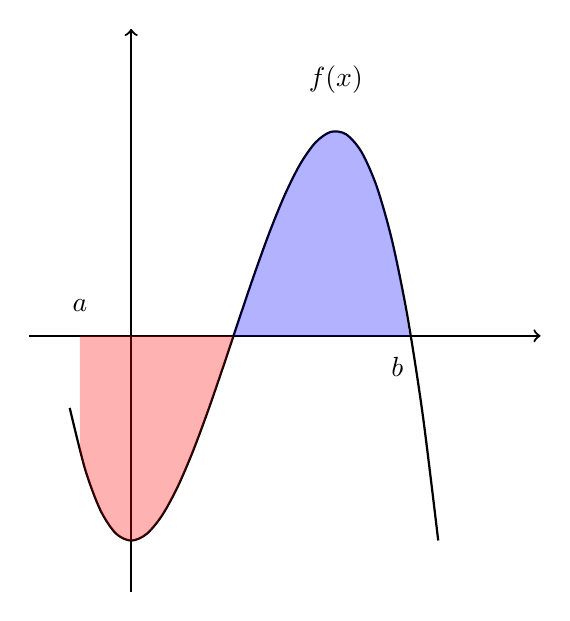
\begin{tikzpicture}[scale=1.3]
		\draw[thick,->] (-1,0) -- (4,0);
		\draw[thick,->] (0,-2.5) -- (0,3);
		
		% Define the function f(x)
		\draw[domain=-0.6:3, smooth, variable=\x, thick]
		plot ({\x}, {-(\x-1)^3 + 3*(\x-1)});
		
		% Shaded area under curve from a to 0
		\fill[red, opacity=0.3]
		(-0.5,0) -- plot[domain=-0.5:0.9, smooth] (\x, {-(\x-1)^3 + 3*(\x-1)}) -- (1,0) -- cycle;
		
		% Shaded area under curve from 0 to b
		\fill[blue, opacity=0.3]
		(1,0) -- plot[domain=0.9:2.6, smooth] (\x, {-(\x-1)^3 + 3*(\x-1)}) -- (2.72,0) -- cycle;
		
		
		% Add labels for a and b
		\node at (-0.5, 0.3) {$a$};
		\node at (2.6,-0.3) {$b$};
		
		% Add label for f(x)
		\node at (2,2.5) {$f(x)$};
		
	\end{tikzpicture}
\end{minipage}

.

\vspace{0.3cm}
\begin{minipage}{0.35\textwidth}
	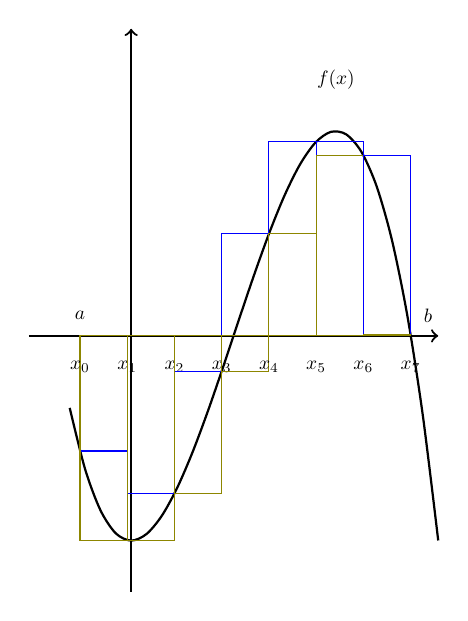
\begin{tikzpicture}[every node/.style={scale=0.7}, scale=1.3]
		% Define the function f(x)
		\def\func{-(\x-1)^3 + 3*(\x-1)}
		
		% Draw axes
		\draw[thick,->] (-1,0) -- (3,0);
		\draw[thick,->] (0,-2.5) -- (0,3);
		
		% Plot the function f(x)
		\draw[domain=-0.6:3, smooth, variable=\x, thick]
		plot ({\x}, {\func});
		
		
		% Add labels for a and b
		\node at (-0.5,0.2) {$a$};
		\node at (2.9,0.2) {$b$};
		
		% Add label for f(x)
		\node at (2,2.5) {$f(x)$};
		
		% Define the points a and b
		\def\a{-0.5}
		\def\b{2.73}
		
		% Calculate the width of each segment
		\pgfmathsetmacro{\width}{(\b-\a)/7}
		
		% Draw the rectangles with maximum height and mark the x_i points
		\foreach \i in {1,...,7} {
				\pgfmathsetmacro{\xprev}{\a + (\i-1)*\width}
				\pgfmathsetmacro{\x}{\a + \i*\width}
				\pgfmathsetmacro{\fxprev}{-(\xprev-1)^3 + 3*(\xprev-1)}
				\pgfmathsetmacro{\fx}{-(\x-1)^3 + 3*(\x-1)}
				\pgfmathsetmacro{\height}{max(\fxprev, \fx)}
				\pgfmathsetmacro{\heightdos}{min(\fxprev, \fx)}
				% Draw the rectangle with yellow outline
				\draw[blue]
				(\xprev, 0) -- (\xprev, \height) -- (\x, \height) -- (\x, 0) -- cycle;
				\draw[olive]
				(\xprev, 0) -- (\xprev, \heightdos) -- (\x, \heightdos) -- (\x, 0) -- cycle;
				% Mark x_i points
				% \draw[dashed] (\x, 0) -- (\x, \height);
				
				\node at (\x, -0.3) {$x_{\i}$};
			}
		% Mark x_0 point
		\node at (\a, -0.3) {$x_0$};
		
	\end{tikzpicture}
\end{minipage}
\begin{minipage}{0.65\textwidth}
	Ahora, definimos la suma superior e inferior asociada a la particion:
	\[
		U = \sum_{i=1}^{n } M_i (x_i - x_{i -1 }) \text{ y } L = \sum_{i=1}^{n } m_i (x_i - x_{i-1}) \text{ (áreas rectangulos)}
	\]
	Observamos que \(L \leq U \) para cualquier particion.
	
	De hecho, si cogemos todas las particiones posibles y nos quedamos con el supremo de \(L \) y el infimo de \(U \), seguimos manteniendo la desigualdad:
	\[
		\sup L \leq \inf U
	\]
\end{minipage}

En el caso de que ambas cantidades sean iguales, diremos que \(f \) es integrable en \([a,b ]\) y definimos la integral como
\[
	\int^{b}_{a} f = \int^{b}_{a} f(x) \; \mathrm{d} x = \sup L = \inf U
\]
Además, definimos \(\int^{a}_b f = - \int^{b}_{a} f \) y \(\int^{a}_{a} f =0 \).

\vspace{1.5cm}
\section{Propiedades de las integrales}
\begin{theorem}
	Sea \(f\colon I \to \R\), con \(I \subseteq \R\). 
	\[
		\text{Si } f \text{ es continua en } [a,b] \Rightarrow f \text{ es integrable en } [a,b].     
	\]
	Además, el área comprendida entre la gráfica de una función continua positiva, el eje \(X \) y las rectas \(x = a \) y \(x = b\), es igual a 
	\[
		\int^{b}_{a} f. 
	\]
\end{theorem}
\begin{proof}
	Tampoco se ha visto en clase. 
\end{proof}
\begin{example}
	\(f(x) = c \), con \(c \in \R\).
	
	Sean \(a,b \in \R \) y consideramos el intervalo \([b,a ]\). Sea \(P = \set{x_0, x_1, \ldots, x_n } \subset [a,b]\).
	\begin{multline*}
		L (f, P) = \sum_{i=1}^{n } m_i (x_i - x_{i-1}) = \sum_{i=1}^{n } c(x_i - x_{i-1}) = c \sum_{i=1}^{n } (x_i - x_{i-1}) = c (x_n - x_0) = c (b-a)
	\end{multline*}
	\[
		U(f, P) = \sum_{i=1}^{n } M_i (x_i - x_{i-1}) = c \sum_{i=1}^{n } (x_i - x_{i-1}) = c(b-a)
	\]
	Por tanto, \(U(f,P) = L(f,P) = c(b-a ) \; \forall P\). Es decir, \(f \) es integrable y \(\int^{b}_{a} f(x)dx = \int^{b}_a c dx  = c(b-a) \).
	\begin{figure}[H]
		\centering
		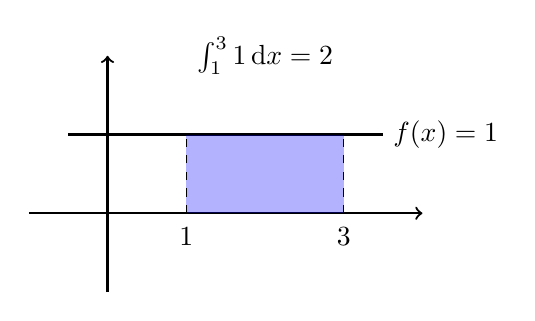
\begin{tikzpicture}
			% Draw axes
			\draw[thick,->] (-1,0) -- (4,0);
			\draw[thick,->] (0,-1) -- (0,2);
			
			% Plot the function f(x) = 1
			\draw[domain=-0.5:3.5, smooth, variable=\x, thick]
			plot ({\x}, {1}) node[right] {$f(x) = 1$};
			
			% Shaded area under the curve from x = 1 to x = 3
			\fill[blue, opacity=0.3]
			(1,0) -- (1,1) -- (3,1) -- (3,0) -- cycle;
			
			% Add dashed lines to show the limits of integration
			\draw[dashed] (1,0) -- (1,1);
			\draw[dashed] (3,0) -- (3,1);
			
			% Add labels for the limits of integration
			\node at (1,-0.3) {$1$};
			\node at (3,-0.3) {$3$};
			
			% Label the integral
			\node at (2,2) {$\int_{1}^{3} 1 \, \mathrm{d} x = 2$};
			
		\end{tikzpicture}
	\end{figure}
\end{example}
\begin{example}
	\(\int^{1}_{0} x dx  = ? \). Consideramos una particion \(P = \set{0, \frac{1}{n}, \frac{2}{n}, \frac{3}{n}, \ldots, \frac{n}{n}}\). Esta particion es equiespacial ya que la diferencia entre cada elemento es siempre \(\frac{1}{n }\). Por ejemplo, si \(n = 4 \) la particion seria \(P_4 = \left \{0,\frac{1}{4}, \frac{2}{4}, \frac{3}{4}, \frac{4}{4}\right \}\). En este caso,
	\begin{multline*}
		U(x, P_4) = M_1 (x_1 - x_0) + M_2 (x_2 - x_1) + M_3(x_3 - x_2) + M_4 (x_4 - x_3) = \\ = x_1 \cdot \frac{1}{4} + x_2 \cdot \frac{1}{4} + x_3 \cdot \frac{1}{4} + x_4 \cdot \frac{1}{4} =  \frac{1}{4} \cdot \frac{1}{4} + \frac{1}{2} \cdot \frac{1}{4} + \frac{3}{4} \cdot \frac{1}{4} + 1 \cdot \frac{1}{4}
	\end{multline*}
	\begin{multline*}
		L(x, P_4) = m_1 (x_1 - x_0) + m_2 (x_2 - x_1) + m_3(x_3 - x_2) + m_4 (x_4 - x_3) = \\ = x_0 \cdot \frac{1}{4} + x_1 \cdot \frac{1}{4} + x_2 \cdot \frac{1}{4} + x_3 \cdot \frac{1}{4} =  0 \cdot \frac{1}{4} + \frac{1}{4} \cdot \frac{1}{4} + \frac{1}{2} \cdot \frac{1}{4} + \frac{3}{4} \cdot \frac{1}{4}
	\end{multline*}
	Ahora vemos el caso general. Para \(P_n \),
	\[
		U(x, P_n) = \sum_{j =1}^{n } M_j \cdot (x_j - x_{j-1}) = \sum_{j =1}^{n } x_j \cdot \frac{1}{n} = \sum_{j =1}^{n } \frac{j}{n} \cdot \frac{1}{n} = \frac{1}{n^{2} }  \sum_{j =1}^{n } j
	\]
	\[
		L(x, P_n) = \sum_{j =1}^{n } m_j \cdot (x_j - x_{j-1}) = \sum_{j =1}^{n } x_{j-1} \cdot \frac{1}{n} = \sum_{j =1}^{n } \frac{j-1}{n} \cdot \frac{1}{n} = \frac{1}{n^{2} }  \sum_{j =1}^{n } (j - 1)
	\]
	Por tanto, nos queda que \(U(x, P_n) = \frac{1}{n^{2} } \sum_{j =1}^{n } j\) y \(L(x,P_n) = \frac{1}{n^{2} } \sum_{j =1}^{n } (j - 1)\).
	
	Sea \(U(f) = \inf (U(f,P)) \) y \(L(f) = \sup (L(f,P ))\). Es obvio que \(L(f) \leq U(f )\). En particular,
	\[
		\frac{1}{n^{2} } \sum_{j =1}^{n } (j - 1) = L(f, P_n) \leq L(f) \leq U(f) \leq U(f,P_n) = \frac{1}{n^{2} } \sum_{j =1}^{n } j
	\]
	Ademas, \(\sum_{j =1}^{n } j = \frac{n (n + 1)}{2 }\) y \(\sum_{j =1}^{n } (j - 1) = \sum_{j=1}^{n} j - \sum_{j =1}^{n } 1 = \frac{n(n-1)}{2} - n \).
	
	Por tanto, \(L(f, P_n) = \frac{1}{n^{2} } \cdot \frac{n(n + 1)}{2} - n = \frac{n^{2} + n}{2n^{2} } - \frac{n }{n^{2} } \overset{n \rightarrow \infty}{\longrightarrow} \frac{1}{2}\) y \(U(f,P_n) = \frac{1}{n^{2} } \frac{n(n + 1)}{2} = \frac{n^{2} + n }{2n^{2} } \overset{n \rightarrow \infty}{\longrightarrow} \frac{1}{2}\).
	
	Entonces, \(L(f) = U(f) = \frac{1}{2}\) y \(f \) es integrable \(\Rightarrow \int^{1}_{0} x dx = \frac{1}{2} \).
	
	\begin{figure}[H]
		\centering
		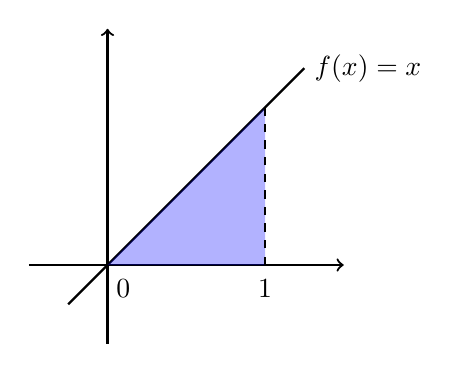
\begin{tikzpicture}
			% Draw axes
			\draw[thick,->] (-1,0) -- (3,0);
			\draw[thick,->] (0,-1) -- (0,3);
			
			% Plot the function f(x) = x
			\draw[domain=-0.5:2.5, smooth, variable=\x, thick]
			plot ({\x}, {\x}) node[right] {$f(x) = x$};
			
			% Shaded area under the curve from x = 0 to x = 2
			\fill[blue, opacity=0.3]
			(0,0) -- (0,0) -- (2,2) -- (2,0) -- cycle;
			
			% Add dashed lines to show the limits of integration
			\draw[dashed] (0,0) -- (0,0);
			\draw[dashed] (2,0) -- (2,2);
			
			% Add labels for the limits of integration
			\node at (0.2,-0.3) {$0$};
			\node at (2,-0.3) {$1$};
			
			% Label the integral
			% \node at (1.5,3.5) {$\int_{0}^{1} x \, \mathrm{d} x = \frac{1}{2}$};
			
		\end{tikzpicture}
	\end{figure}
\end{example}

\begin{proposition}
	Sean \(f \) y \(g \) integrables en \([a,b ]\), entonces: 
	\begin{itemize}
		\item \(f + g \) es integrable en \([a,b ]\) y \(\int^{b}_a (f + g) = \int^{b}_a f + \int^{b}_a g \).
		\item \(\lambda f \) es integrable en \([a,b ]\) y \(\int^{b}_a \lambda f = \lambda \int^{b}_a f\).
		\item \(\left\vert f  \right\vert \) es integrable en \([a,b ]\) y \(\int^{b}_a f \leq \int^{b}_a \left\vert f  \right\vert . \)
		\item \(f \cdot g \) es integrable en \([a,b ]\) pero, en general, \(\int^{b}_a f \cdot g \neq \int^{b}_a f \cdot \int^{b}_a g\).
	\end{itemize}
\end{proposition}
\begin{proposition}
	Sea \(f\colon I \to \R\), \(I \subset \R\) y \(a,b,c \in \R\) con \(a \leq  b \leq  c\) . Entonces 
	\[
		f \text{ es integrable en } [a,c] \iff f \text{ es integrable en } [a,b] \text{ y } [b,c].  
	\]
	Además, \(\int^{c}_a f = \int^{b}_{a} f + \int^{c}_b f\).  
\end{proposition}
\begin{proposition}
	Sean \(f \) y \(g \) integrables en \([a,b ]\): 
	\begin{itemize}
		\item Si \(f(x) \geq 0 \quad  \forall x \in [a,b]\), entonces \(\int^{b}_a f \geq 0\).
		\item Si \(f(x) \geq g(x) \quad \forall x \in [a,b]\), entonces \(\int^{b}_a f \geq \int^{b}_a g\).
	\end{itemize}
\end{proposition}
\section{Teoremas sobre Integrales}
\begin{theorem}[Regla de Barrow]
	Sean \(f \) y \(F \) continuas en \([a,b ]\) y \(F \) derivable en \((a,b )\) tal que \(F^\prime (x) = f(x) \; \forall x \in (a,b)\). Entonces, 
	\[
		\int^{b}_a f(x) \; \mathrm{d}x = \left [F(x) \right ]^{b}_a = F(b) - F(a)
	\]
\end{theorem}
\begin{theorem}[fundamental del calculo]
	Si \(f \) es continua en \([a,b ]\) entonces existe una funcion \(F \) tal que \(F^\prime (x) = f(x) \; \forall x \in [a,b ]\).
\end{theorem}
\begin{proof}
	Sabemos que si \(f \) es continua en \([a,b ]\) entonces es integrable en \([a,b ]\). Dado \(x \in [a,b ]\), tambien se tiene que \(f \) es integrable en \([a,x ]\).
	
	Definimos \(F(x) = \int^{x}_a f(t) dt  \). Veamos que \(F(x )\) es derivable en \(c \in [a,b ]\) es decir, \(F^\prime (c) = \lim\limits_{h  \to 0 } \frac{F(c + h) - F(c )}{h} = f(c) \Rightarrow \forall \varepsilon > 0 \;\exists \delta > 0\) t.q. si \(h \in (-\delta, \delta), h \neq 0,\) se cumple \(\left\vert \frac{F(c+h) - F(c)}{h} - f(c) \right\vert < \varepsilon \).
	
	\begin{align*}
		\left\vert \frac{F(c+h) - F(c)}{h} - f(c) \right\vert & = \left\vert \frac{\int^{c+h}_a f(t )dt  - \int^{c}_a f(t) dt }{h} - f(c) \right\vert = \left\vert \frac{\int^{c+h}_c f(t) dt }{h} - f(c) \right\vert                                        \\
		                                                      & = \left\vert \frac{\int^{c +h}_c f(t) dt }{h} - f(c ) \right\vert = \left\vert \frac{\int^{c + h}_c f(t)dt }{h} - f(c) \cdot \underbrace{\frac{1}{h} \int^{c +h}_{c} 1 dt }_{=1} \right\vert \\ & = \left\vert \frac{1}{h} \cdot \left [ \int^{c + h}_c f(t) dt - f(c) \cdot \int^{c + h}_{c} 1 dt   \right ] \right\vert = \left\vert \frac{1}{h} \cdot \int^{c +h}_c f(t) - f(c) dt   \right\vert \\ & \leq \left\vert \frac{1}{h } \right\vert \int^{c + h}_{c} \left\vert f(t) - f(c ) \right\vert dt = \left\vert \frac{F(c + h ) - F(c)}{h} - f(c) \right\vert  \overset{?}{<} \varepsilon
	\end{align*}
	Sea \(\varepsilon > 0 \). Como \(f \) es continua en \(c \), entonces \(\exists \delta > 0 \) tal que \(\forall t \in (c - \delta, c + \delta)\), \(t \neq c\), se cumple \(\left\vert f(t) - f(c ) \right\vert < \varepsilon\). Luego \(\forall h \in (- \delta, \delta ), h \neq 0\), suponemos que \(h > 0 \) (similar si \(h < 0 \)) y tenemos que    
	\begin{align*}
		\left\vert \frac{F(c + h) - F(c )}{h} - f(c) \right\vert & \leq \frac{1}{\left\vert h  \right\vert } \cdot \int^{c + h}_c \left\vert f(t) - f(c ) \right\vert dt < \frac{1}{h} \cdot \int^{c + h}_c \varepsilon dt \\ & =  \frac{1}{h} \cdot \varepsilon \cdot \int^{c + h}_c 1 dt = \frac{1}{h} \cdot \varepsilon \cdot h = \varepsilon 
	\end{align*}
	*Borrador, falta reescribirlo*
\end{proof}

Integración por partes, cambios de variable.